\documentclass[twoside,11pt,fleqn]{book}

\usepackage[switch*,pagewise]{lineno}
\usepackage[dvipdfmx]{graphicx}
\usepackage[dvipdfmx]{color}

\usepackage{titlesec}
\setcounter{secnumdepth}{4}

\usepackage[nottoc,notlot,notlof]{tocbibind}

\usepackage[framemethod=TikZ]{mdframed}
\newmdenv[%
backgroundcolor=red!8,
linecolor=red,
outerlinewidth=1pt,
%roundcorner=5mm,
skipabove=\baselineskip,
skipbelow=\baselineskip,
]{mdbox}

\usepackage[dvipdfmx]{hyperref}
\usepackage{pxjahyper}
\hypersetup{colorlinks, citecolor=black, filecolor=black, linkcolor=blue, urlcolor=black}
%\usepackage{bookmark}

\usepackage[toc,nonumberlist]{glossaries}

%\usepackage{floatrow}
%\floatsetup[table]{capposition=top}
%\newfloatcommand{capbtabbox}{table}[][\FBwidth]

\usepackage{array}
\newcolumntype{L}[1]{>{\raggedright\let\newline\\\arraybackslash\hspace{0pt}}m{#1}}
\newcolumntype{C}[1]{>{\centering\let\newline\\\arraybackslash\hspace{0pt}}m{#1}}
\newcolumntype{R}[1]{>{\raggedleft\let\newline\\\arraybackslash\hspace{0pt}}m{#1}}
\usepackage{amssymb}

\usepackage{placeins}
\usepackage{multirow}
\usepackage[toc,page]{appendix}
\usepackage{fancyvrb}
\usepackage{xcolor}
\usepackage{listings}
\usepackage{url}
\usepackage[normalem]{ulem}
\usepackage{soul}
\DeclareRobustCommand{\hsout}[1]{\texorpdfstring{\sout{#1}}{#1}}

\newcommand\textttw[1]{\mathchardef\UrlBreakPenalty=100\mathchardef\UrlBigBreakPenalty=100\url{#1}}
%%%%%%%%%%%%%%%%%%%%%%%%%%%%%%%%%%%%%%%%%%%%%%%%%%%%%%
% Define a new command \subsubsubsection
\titleclass{\subsubsubsection}{straight}[\subsection]

\newcounter{subsubsubsection}[subsubsection]
\renewcommand\thesubsubsubsection{\thesubsubsection.\arabic{subsubsubsection}}
\renewcommand\theparagraph{\thesubsubsubsection.\arabic{paragraph}} % optional; useful if paragraphs are to be numbered

\titleformat{\subsubsubsection}
  {\normalfont\normalsize\bfseries}{\thesubsubsubsection}{1em}{}
\titlespacing*{\subsubsubsection}
{0pt}{3.25ex plus 1ex minus .2ex}{1.5ex plus .2ex}

\makeatletter
\renewcommand\paragraph{\@startsection{paragraph}{5}{\z@}%
  {3.25ex \@plus1ex \@minus.2ex}%
  {-1em}%
  {\normalfont\normalsize\bfseries}}
\renewcommand\subparagraph{\@startsection{subparagraph}{6}{\parindent}%
  {3.25ex \@plus1ex \@minus .2ex}%
  {-1em}%
  {\normalfont\normalsize\bfseries}}
\def\toclevel@subsubsubsection{4}
\def\toclevel@paragraph{5}
\def\toclevel@paragraph{6}
\def\l@subsubsubsection{\@dottedtocline{4}{7em}{4em}}
\def\l@paragraph{\@dottedtocline{5}{10em}{5em}}
\def\l@subparagraph{\@dottedtocline{6}{14em}{6em}}
\makeatother
%%%%%%%%%%%%%%%%%%%%%%%%%%%%%%%%%%%%%%%%%%%%%%%%%%%%%%
\long\def\comment#1{}

\usepackage{etoolbox}
\usepackage{datetime}

\DefineVerbatimEnvironment{VerbX}{Verbatim}{}

\newenvironment{myverbt}
  {\VerbatimEnvironment
   \par\VerbX}
  {\endVerbX }

\newenvironment{myverbf}
  {\VerbatimEnvironment
   \par\vspace{\dimexpr-1.2\baselineskip\relax}
   \VerbX}
  {\endVerbX }


%   \par\vspace{\dimexpr-1.2\topsep-1.2\partopsep\relax}

% WG合意内容からの差異を赤字で表示
\ifx \HLDIFFWG y
\long\def\DIFFWG#1{\textcolor{red}{#1}}
\else
\long\def\DIFFWG#1{#1}
\fi

% 運用ソフト連携部抜粋からの差異を赤字で表示
\ifx \HLDIFFOPS y
\long\def\ADDOPS#1{\textcolor{red}{#1}}
\long\def\RMOPS#1{\textcolor{red}{\sout{#1}}}
\else
\long\def\ADDOPS#1{#1}
\long\def\RMOPS#1{}
\fi

% 2017/6/30版と2017/7/21版の差異を赤字で表示
\ifx \HLDIFFJUL y
\long\def\DIFFJUL#1{\textcolor{red}{#1}}
\else
\long\def\DIFFJUL#1{#1}
\fi

% 2017/7/21版と2017/7/31版の差異を赤字で表示
\ifx \HLDIFFJULTWO y
\long\def\ADDJULTWO#1{\textcolor{red}{#1}}
\long\def\MODJULTWO#1{\textcolor{red}{#1}}
\long\def\RMJULTWO#1{\textcolor{red}{\hsout{#1}}}
\long\def\ADDJULTWOS#1{\textcolor{red}{【追加】#1}}
\long\def\MODJULTWOS#1{\textcolor{red}{【変更】#1}}
\long\def\RMJULTWOS#1{\textcolor{red}{【削除】#1}}
\else
\long\def\ADDJULTWO#1{#1}
\long\def\MODJULTWO#1{#1}
\long\def\RMJULTWO#1{}
\long\def\ADDJULTWOS#1{#1}
\long\def\MODJULTWOS#1{#1}
\long\def\RMJULTWOS#1{#1}
\fi

% 2017/7/31版と2017/8/31版の差異を赤字で表示
\ifx \HLDIFFAUG y
\long\def\ADDAUG#1{\textcolor{red}{#1}}
\long\def\MODAUG#1{\textcolor{red}{#1}}
\long\def\RMAUG#1{\textcolor{red}{\hsout{#1}}}
\long\def\ADDAUGS#1{\textcolor{red}{【追加】#1}}
\long\def\MODAUGS#1{\textcolor{red}{【変更】#1}}
\long\def\RMAUGS#1{\textcolor{red}{【削除】#1}}
\else
\long\def\ADDAUG#1{#1}
\long\def\MODAUG#1{#1}
\long\def\RMAUG#1{}
\long\def\ADDAUGS#1{#1}
\long\def\MODAUGS#1{#1}
\long\def\RMAUGS#1{#1}
\fi

% V1.2.6とV1.2.7の差異(V1.3.0とV1.3.1の差異)を赤字で表示
\ifx \HLDIFFSEP y
\long\def\ADDSEP#1{\textcolor{red}{#1}}
\long\def\MODSEP#1{\textcolor{red}{#1}}
\long\def\RMSEP#1{\textcolor{red}{\hsout{#1}}}
\long\def\ADDSEPS#1{\textcolor{red}{【追加】#1}}
\long\def\MODSEPS#1{\textcolor{red}{【変更】#1}}
\long\def\RMSEPS#1{\textcolor{red}{【削除】#1}}
\else
\long\def\ADDSEP#1{#1}
\long\def\MODSEP#1{#1}
\long\def\RMSEP#1{}
\long\def\ADDSEPS#1{#1}
\long\def\MODSEPS#1{#1}
\long\def\RMSEPS#1{#1}
\fi

% 疑似ファイルシステム関連仕様変更(2018/7/9, 1.5.1)の差異を赤字で表示
\ifx \HLDIFFPROC y
\long\def\ADDPROC#1{\textcolor{red}{#1}}
\long\def\MODPROC#1{\textcolor{red}{#1}}
\long\def\RMPROC#1{\textcolor{red}{\hsout{#1}}}
\long\def\ADDPROCS#1{\textcolor{red}{【追加】#1}}
\long\def\MODPROCS#1{\textcolor{red}{【変更】#1}}
\long\def\RMPROCS#1{\textcolor{red}{【削除】#1}}
\else
\long\def\ADDPROC#1{#1}
\long\def\MODPROC#1{#1}
\long\def\RMPROC#1{}
\long\def\ADDPROCS#1{#1}
\long\def\MODPROCS#1{#1}
\long\def\RMPROCS#1{#1}
\fi

% 一つ前のバージョンとの差異を赤字で表示
\ifx \HLDIFFPREV y
\long\def\ADDPREV#1{\textcolor{red}{#1}}
\long\def\MODPREV#1{\textcolor{red}{#1}}
\long\def\RMPREV#1{\textcolor{red}{\hsout{#1}}}
\long\def\ADDPREVS#1{\textcolor{red}{【追加】#1}}
\long\def\MODPREVS#1{\textcolor{red}{【変更】#1}}
\long\def\RMPREVS#1{\textcolor{red}{【削除】#1}}
\else
\long\def\ADDPREV#1{#1}
\long\def\MODPREV#1{#1}
\long\def\RMPREV#1{}
\long\def\ADDPREVS#1{#1}
\long\def\MODPREVS#1{#1}
\long\def\RMPREVS#1{#1}
\fi

% diff rc3 rc4
\ifx \HLDIFFRCF y
\long\def\ADDRCF#1{\textcolor{red}{#1}}
\long\def\MODRCF#1{\textcolor{red}{#1}}
\long\def\RMRCF#1{\textcolor{red}{\hsout{#1}}}
\long\def\ADDRCFS#1{\textcolor{red}{【追加】#1}}
\long\def\MODRCFS#1{\textcolor{red}{【変更】#1}}
\long\def\RMRCFS#1{\textcolor{red}{【削除】#1}}
\else
\long\def\ADDRCF#1{#1}
\long\def\MODRCF#1{#1}
\long\def\RMRCF#1{}
\long\def\ADDRCFS#1{#1}
\long\def\MODRCFS#1{#1}
\long\def\RMRCFS#1{#1}
\fi

\pagestyle{plain}
\setcounter{tocdepth}{3}
\marginparwidth 0pt
\oddsidemargin=.25in
\evensidemargin  .25in
\marginparsep 0pt
\topmargin=-.5in
\textwidth=6.0in
\textheight=9.0in
\parindent=2em

% \chapter{Terms}
% 本章では用語とその定義を説明する。
% \begin{description}
\newglossaryentry{レイテンシコア}{name=レイテンシコア, description={シングルスレッド実行における遅延削減に重点を置いて開発されたプロセッサのコア。}}
%または結果が出始めるまでのコストであるスタートアップコストを小さくすることに重点を置いて開発されたプロセッサのコア。
\newglossaryentry{ノード}{name=ノード, description={一つ以上のプロセッサ、それらに接続されたRAM、それらに接続されたI/Oデバイスから構成されるコンピュータで、スーパーコンピュータはこれらの群で構成される。}}
\newglossaryentry{OSサービス}{name=OSサービス, description={プロセス管理、メモリ管理、システムコールなどアプリケーションに提供するハードウェア仮想化サービス。}}
\newglossaryentry{汎用OS}{name=汎用OS, description={Linuxに代表される、主にサーバ用途のOS。}}
\newglossaryentry{軽量カーネル、Light-Weight Kernel (LWK)}{name=軽量カーネル、Light-Weight Kernel (LWK), description={アプリケーション実行に必要な最低限の機能のみ備えるOSカーネル。}}
\newglossaryentry{Full Wieght Kernel (FWK)}{name=Full Wieght Kernel (FWK), description={汎用OSが提供する全てのOSサービスを単体で提供するOSカーネル。}}
\newglossaryentry{McKernel}{name=McKernel, description={将来のメニーコアアーキテクチャ型スーパーコンピュータシステム向けのOSとして東京大学で開発が開始され理化学研究所が開発を引き継いでいるOSカーネル。}}
\newglossaryentry{Interface for Heterogeneous Kernels (IHK)}{name=Interface for Heterogeneous Kernels (IHK), description={ノード上の複数のパーティションで異種OSカーネルを同時動作させる仕組みを実現するフレームワーク。Linuxカーネルモジュールとして動作するIHK−Master、LWK用ライブラリとして動作するIHK−Slaveから構成される。また、IHK使用者に対してはLinuxのカーネルモジュール、LWK用ライブラリとして提供される。}}
\newglossaryentry{IHK-Master}{name=IHK-Master, description={Linuxカーネルモジュールとして動作し、ノードのブート、パーティション作成、LWK起動、LWKとの通信の機能を提供するIHKのモジュール。}}
\newglossaryentry{IHK-Slave}{name=IHK-Slave, description={LWKのモジュールとして動作し、IHK−Masterとの通信の機能を提供するIHKのモジュール。}}
\newglossaryentry{Inter-Kernel Communication (IKC)}{name=Inter-Kernel Communication (IKC), description={IHK-MasterとIHK−Slaveにより提供される異種カーネル間の通信。}}
\newglossaryentry{ジョブ}{name=ジョブ, description={一連のノード操作またはプロセス群の実行。}}
\newglossaryentry{ジョブスケジューラ}{name=ジョブスケジューラ, description={ユーザからのリクエストを受け、ジョブにスーパーコンピュータシステムのノードを割り当て、また割り当てられたノード群の上でジョブを実行するソフトウェアシステム。}}
\newglossaryentry{資源}{name=資源, description={アプリケーション実行の際にユーザによって一定時間占有される、物理コア、RAM、HDDなどのスーパーコンピュータの構成要素。}}
\newglossaryentry{パーティショニング・パーティション}{name=パーティショニング・パーティション, description={ノードの資源を分割すること。または分割されてできた資源サブセットのこと。McKernelの実行の際には物理コアおよびメモリを分割する。}}
\newglossaryentry{mcctrl}{name=mcctrl, description={Linuxのカーネルモジュールとして動作し、McKernelと通信を行うMcKernelのモジュール。}}
\newglossaryentry{mcexec}{name=mcexec, description={Linuxのユーザプログラムとして動作し、McKernelのプロセスの管理を行うMcKernelのモジュール。}}
\newglossaryentry{buitin構成}{name=buitin構成, description={一つのプロセッサを複数のパーティションに分けて、一つのパーティションでLinuxなどのOSサービスを提供するOSカーネルを動作させ、他のパーティションでLWKを動作させる構成。}}
\newglossaryentry{attached構成}{name=attached構成, description={プロセッサでLinuxなどのOSサービスを提供するOSカーネルを動作させ、PCIバスなどのI/Oバスで接続されたデバイスでLWKを動作させる構成。}}
\newglossaryentry{McKernelインスタンス}{name=McKernelインスタンス, description={独立したパーティション内で他のOSカーネルと資源を共有せずに動作するMcKernelの実体。}}
\newglossaryentry{アプリ特化カーネル}{name=アプリ特化カーネル, description={アプリケーションの高速化ができるように最適化されたOSカーネル。例えばタイムシェアリング機能をなくすことでOSノイズを低減することでアプリケーションの高速化を行ったカーネル。}}
\newglossaryentry{カーネル切り替え}{name=カーネル切り替え, description={複数のアプリ特化カーネルから一つ選択してそれを動作させること。}}
\newglossaryentry{Non-Uniform Memory Access (NUMA)}{name=Non-Uniform Memory Access (NUMA), description={メモリアクセスについて、ある一つのコアから観測される遅延やバンド幅がメモリ領域によって異なるアーキテクチャ。}}
\newglossaryentry{NUMA-node}{name=NUMA-node, description={メモリコントローラとDRAMの組み合わせなどのメモリアクセスを行うハードウェアモジュールのこと。}}
\newglossaryentry{インターコネクト}{name=インターコネクト, description={ノードとノードを結ぶ通信路のこと。}}
\newglossaryentry{procfs}{name=procfs, description={Linuxの提供する、ファイルシステムをインターフェイスとするカーネルからの情報提示及びカーネルへの指示機構。}}
\newglossaryentry{Linux API}{name=Linux API, description={アプリケーションがLinuxカーネルの機能を利用する際の規則のこと。例えば、システムコールの名前、その呼び出しの引数の数、型、返り値の型、その作用が挙げられる。}}
\newglossaryentry{モジュール}{name=モジュール, description={ソフトウェアのある程度独立して動作する部分。}}
\newglossaryentry{コモディティクラスタ}{name=コモディティクラスタ, description={広く販売されているコンピュータを複数接続して構成したクラスタ型コンピュータ。例としてはIntel社製プロセッサを搭載したPC/ATアーキテクチャのマシンをInfiniBandネットワークで複数接続して構成したコンピュータが挙げられる。}}
\newglossaryentry{形式手法}{name=形式手法, description={ステートマシンとステートを用いた論理記述を用いて特定の条件が成立する可能性の有無を証明する手法。}}
\newglossaryentry{アノテーション}{name=アノテーション, description={ソースコードに埋め込む、補助的な動作や条件などを表す記述。}}
\newglossaryentry{アサーション}{name=アサーション, description={成立すべき条件を表す記述。}}
\newglossaryentry{Open Source Software (OSS)}{name=Open Source Software (OSS), description={ソースが公開されているソフトウェア。}}
\newglossaryentry{Linuxオンリーモード}{name=Linuxオンリーモード, description={運用者またはシステムソフトウェア開発者視点でのノードの状態であって、Linuxのみが動作する状態のこと。}}
\newglossaryentry{McKernelモード}{name=McKernelモード, description={運用者またはシステムソフトウェア開発者視点でのノードの状態であって、LinuxとMcKernelが動作する状態のこと。}}
\newglossaryentry{Linux動作モード}{name=Linux動作モード, description={ユーザ視点でのアプリの動作形態であって、Linuxのみが動作するノードを用いるという動作形態のこと。}}
\newglossaryentry{McKernel動作モード}{name=McKernel動作モード, description={ユーザ視点でのアプリの動作形態であって、LinuxとMcKernelが動作するノードを用いるという動作形態のこと。}}
\newglossaryentry{ジョブ資源管理機能}{name=ジョブ資源管理機能, description={ノードにジョブを起動する、1ジョブに対して一つ選択される代表ノードで動作するプロセス。}}
\newglossaryentry{Process Launch Environment (PLE)}{name=Process Launch Environment (PLE), description={複数ノードにプロセスを起動する仕組み。}}
%各ノードでプロセス起動指示を待つデーモンと、このデーモンに指示を与える\texttt{mpiexec}などのツールからなる。
% \end{description}

\makeglossaries

\begin{document}
%\pagenumbering{roman}
\title{Interface for Heterogeneous Kernels (IHK) Specifications\\
  Version 1.7.1-0.93
}

\author{Masamichi Takagi, Balazs Gerofi, Tomoki Shirasawa, Gou Nakamura\\ and Yutaka Ishikawa}

\def\gb{\penalty10000\hskip 0pt plus 8 em\penalty4800\hskip 0pt plus-8em\penalty10000}

\newcommand{\typefacetype}[1]{\gb{\sf #1}}
\newcommand{\subtype}[1]{\textsf{\textbf{#1}}}
\newcommand{\typefacearg}[1]{\gb{\sf #1}}
\newcommand{\declarefunc}[1]{{\raggedright \hangindent 7em\hangafter=1\tt #1 \par \vspace{0.0in}}}
\newcommand{\funcarg}[3]{\item[\hbox to 70pt{\typefacearg{#1} \hfill} \typefacetype{#2}\hfill]{\small #3}}
\newcommand{\typefield}[2]{\item[\hbox to 70pt{\typefacearg{#1} \hfill} \hfill]{\small #2}}
\newcommand{\IN}[0]{{\small \bf{input}}}
\newcommand{\OUT}[0]{{\small \bf{output}}}
\newcommand{\INOUT}[0]{{\small \bf{inout}}}
%\newcommand{\startchap}[0]{\cleardoublepage}

\newlength{\codeSpace}
\setlength{\codeSpace}{.4cm}

\newenvironment{funcdef}[0]{
%\vspace{\codeSpace}
\noindent
\samepage
   \begin{list}
{}{
      %\setlength{\leftmargin}{200pt}
      \setlength{\leftmargin}{100pt}
      %\setlength{\labelwidth}{180pt}
      \setlength{\labelwidth}{80pt}
      \setlength{\labelsep}{10pt}
      \setlength{\itemindent}{0pt}
      \setlength{\itemsep}{0pt}
      \setlength{\topsep}{5pt}
   }
}
{
   \end{list}
%   \vspace{\codeSpace}
}
\newenvironment{structdef}[0]{
%\vspace{\codeSpace}
\noindent
\samepage
   \begin{list}
{}{
      \setlength{\leftmargin}{80pt}
      \setlength{\labelwidth}{60pt}
      \setlength{\labelsep}{10pt}
      \setlength{\itemindent}{0pt}
      \setlength{\itemsep}{0pt}
      \setlength{\topsep}{5pt}
   }
}
{
   \end{list}
   \vspace{\codeSpace}
}

\newdate{date}{18}{01}{2021}
\date{\displaydate{date}}
\maketitle

\tableofcontents
\listoffigures   
%\listoftables   

\linenumbers

\chapter{\MODAUGS{IHK外部仕様}}
\section{\MODAUGS{概要}}

Interface for Heterogeneous Kernels (IHK) is a low-level software
infrastructure, which enables partitioning node resources and the
management of lightweight kernels on subsets of the resources.
This section introduces the basic architecture of IHK and gives a brief
overview of its main components.
An overview of the IHK architecture is shown in Figure \ref{fig:ihk-overall}.

\begin{figure}[h!]
\centerline{
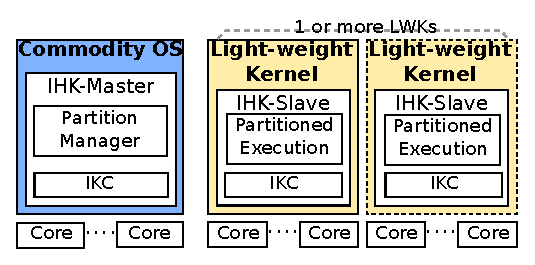
\includegraphics[width=0.60\linewidth]{figs/ihk-design.eps}
}
\caption{\textbf{Architectural overview of IHK components.}}
\label{fig:ihk-overall}
\end{figure}

IHK categorizes kernels in two types: a master kernel and the slave kernels
(i.e., lightweight kernels).
The master kernel is a kernel that is booted in the node first through the
normal booting process,
for example, booted from BIOS or UEFI, and is typically a
commodity operating system, it is Linux in the rest of this document.
Slave kernels are kernels that are booted from the master kernel.
IHK's components in the master and slave kernels are called IHK-master and
IHK-slave\footnote{The terms ``IHK-slave'' and ``co-kernel'' are used interchangably.}, respectively.

Resource partitioning, the management and bootstrapping of lightweight slave
kernels are implemented in IHK-master,
while support for executing over a partition of resources
is implemented in IHK-slave.
A low-level communication facility called IHK-IKC is present
both in IHK-master and IHK-Slave.

\subsection{\MODAUGS{管理者向け機能}}
\label{sec:lwk_management}

This section discusses the functionalities and components of IHK-master.
The resource partitioning mechanism
provided by the implementation in the Linux kernel is also explained.

IHK-master consists of two types of modules. \textit{IHK-master core} provides
the basic IHK framework and management infrastructure.
It is required for registering/removing the so called \textit{IHK-master drivers}
(discussed below) and provides administration interface
through device files and ioctl() APIs for:

\begin{itemize}
\item Managing devices.
\item Managing OS kernel instances.
\end{itemize}

In particular, the IHK-master core module enables in-kernel interfaces
(by means of exporting a set of IHK specific Linux kernel functions)
which allow registration and de-registration of IHK-master drivers.

\textit{IHK-master drivers} represent resources, such as CPU cores of
an SMP chip along with the physical memory of the given node or
PCI-Express attached co-processors.
Specifically, the current IHK implementation in Linux provides one
type of IHK-master drivers:

\begin{itemize}
% \item \textit{IHK-attached:} Enables configuration and interaction with
% a co-processor attached through PCI Express, at this moment only the
% Intel Xeon Phi is supported.

\item \textit{IHK-SMP x86:} Represents a virtual device that enables
partitioning CPU cores of an x86 (Xeon) SMP chip as well as the physical
memory attached to the node among OS instances.
\end{itemize}

Note, that neither the IHK-master core module, nor the IHK-SMP x86
drivers require any modifications to the Linux kernel.

IHK-master drivers support the abstraction of \textit{IHK devices}, which
essentially represent resources. On top of IHK devices one can create
\textit{IHK OS instances} and use the framework to assign a set of
the underlying resources to the particular OS instance.
As we mentioned earlier, IHK exposes its management interface via device
files which in turn can be controlled with specific command line tools.
Figure \ref{fig:ihk-os_creation} shows the execution steps of an IHK device registration and the creation of an OS instance for x86 (Xeon) SMP chip.


\begin{figure}[h!]
\centerline{
	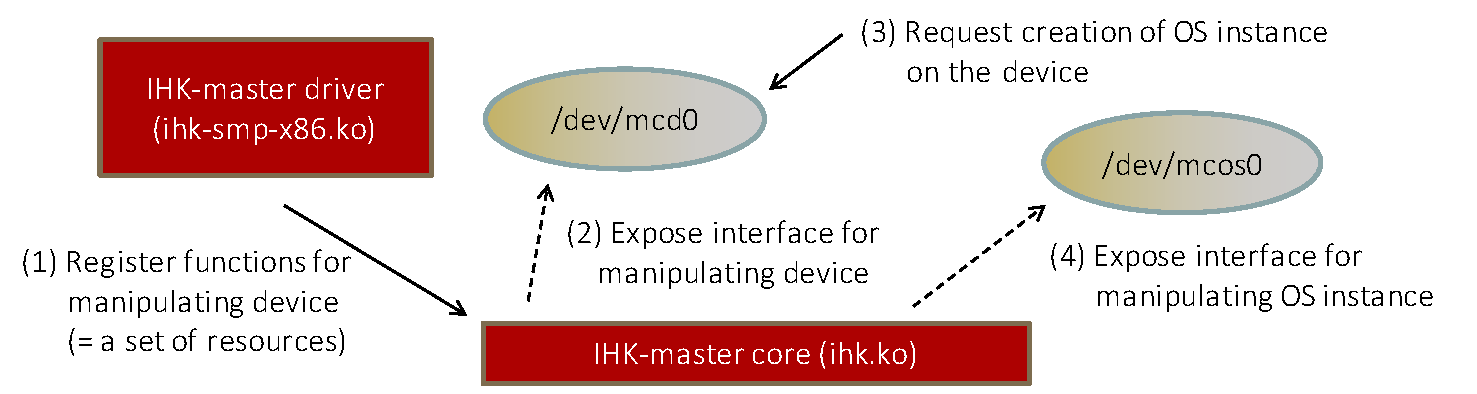
\includegraphics[width=0.90\linewidth]{figs/ihk-os_creation.pdf}
}
\caption{\textbf{Steps of IHK-master driver registration and device file creation.}}
\label{fig:ihk-os_creation}
\end{figure}

The initial state of the figure is right after the IHK-master core module (\texttt{ihk.ko}) has been
loaded. The following four steps are then highlighted:
\begin{enumerate}
	\item Load an IHK-master driver module (\texttt{ihk-smp-x86.ko}), which automatically registers
	itself into the IHK framework.
	\item The IHK framework creates the \texttt{/dev/mcd0} device file,
	which will represent the resources accessible through the inserted
	IHK master driver.
	\item Use the IHK tools (e.g. \texttt{ihkconfig} command or \texttt{ihk\_config} functions) to request creation of an OS instance, which in turn does an ioctl()
	call on the specified IHK device.
	\item The IHK framework creates \texttt{/dev/mcos0} device file, which
	represents an OS instance on top of IHK device \texttt{/dev/mcd0}.
\end{enumerate}

Note the index \texttt{0} in the file names of \texttt{/dev/mcd0} and
\texttt{/dev/mcos0}. The IHK framework allows registration of multiple
IHK-master drivers as well as the creation of multiple OS instances over
a specific IHK device. The index of the corresponding device file is
assigned by the framework automatically.

\begin{figure}[h!]
\centerline{
	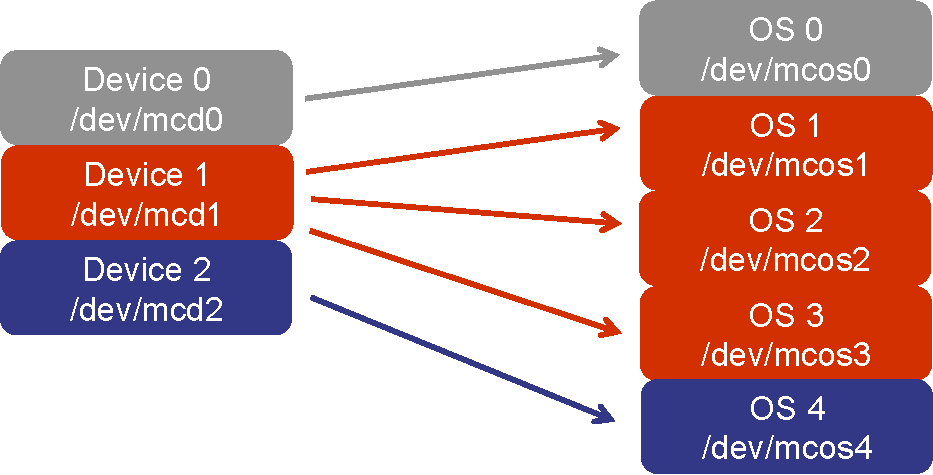
\includegraphics[width=0.50\linewidth]{figs/ihk-dev-os.pdf}
}
\caption{\textbf{Relation between IHK devices and OS instances.}}
\label{fig:ihk-dev-os}
\end{figure}

To emphasize the relation
between OS instances and IHK devices see Figure \ref{fig:ihk-dev-os}.
As shown, \texttt{/dev/mcd1} has multiple OS instances on top of it.


\texttt{x86\_64}アーキテクチャのシステムでの資源管理とOS管理のステップは以下の通り。
\begin{enumerate}
\item コアドライバ\texttt{ihk.ko}と、\texttt{ihk.ko}の開示するインターフェイス経由でシステム依存機能を提供するドライバ\texttt{ihk\_smp\_x86.ko}を\texttt{insmod}する。
\item IHKがCPU資源およびメモリ資源をLinuxから獲得する。この操作を資源の予約と呼ぶ。
\item IHKがOSインスタンスを作成する。
\item IHKがOSインスタンスにCPU資源を割り当てる。
\item IHKがOSインスタンスにメモリ資源を割り当てる。
\item IHKがOSインスタンスにカーネルイメージをロードし、起動する。
\item IHKがOS状態監視のためのファイルディスクリプタをOSインスタンスから取得する。
\item IHKがMcKernelにプロセスを起動する。
\item IHKが必要に応じて、OSインスタンスの統計情報の取得、OSインスタンスの一時停止、OSインスタンスのメモリダンプの採取を行う。
\item IHKがOSインスタンスのカーネルをシャットダウンする。
\item IHKがOSインスタンスに割り当てられたCPU資源およびメモリ資源をIHKに戻す。この操作を資源の解放と呼ぶ。
\item IHKがOSインスタンスを破棄する。
\item IHKがCPU資源およびメモリ資源をLinuxに戻す。この操作を資源の解放と呼ぶ。
\end{enumerate}
IHKは運用ソフトウェアがこれらの操作を行えるようにするコマンド群およびライブラリを提供する。

カーネルモジュール、コマンド、ライブラリの場所は以下の通り。
SMPプロセッサ向け、\texttt{x86\_64}アーキ向けのファイルを記載する。
なお、IHKのインストールディレクトリを\texttt{<ihk\_install>}とする。
\begin{table}[!h]
\footnotesize
\begin{tabular}{|p{0.35\linewidth}|p{0.56\linewidth}|} \hline
\multicolumn{1}{|c}{\textbf{ファイル}}&\multicolumn{1}{|c|}{\textbf{説明}}\\ \hline \hline
\texttt{<ihk\_install>/kmod/ihk.ko}&IHK-master core\\ \hline
\texttt{<ihk\_install>/kmod/ihk-smp-x86.ko}&IHK-master driver\\ \hline
\texttt{<ihk\_install>/include/libihk.h}&資源管理関数およびOS管理関数のヘッダファイル\\ \hline
\texttt{<ihk\_install>/lib/libihk.so}&資源管理関数およびOS管理関数の共有オブジェクト\\ \hline
\texttt{<ihk\_install>/sbin/ihkconfig}&資源管理コマンド\\ \hline
\texttt{<ihk\_install>/sbin/ihkosctl}&OS管理コマンド\\ \hline
\MODAUG{\texttt{<ihk\_install>/sbin/ihkmond}}&\MODAUG{カーネルメッセージのsyslogプロトコルによる\texttt{/dev/log}への転送と、ハングアップの監視とを行うデーモン}\\ \hline
\end{tabular}
\vspace{-0em}
\end{table}
\FloatBarrier

コマンドおよびライブラリのソースコードの場所は以下の通り。
なお、IHKのソースディレクトリを\texttt{<ihk\_src>}とする。
\begin{table}[!h]
\footnotesize
\begin{tabular}{|p{0.35\linewidth}|p{0.56\linewidth}|} \hline
\multicolumn{1}{|c}{\textbf{ファイル}}&\multicolumn{1}{|c|}{\textbf{説明}}\\ \hline \hline
\texttt{<ihk\_src>/linux/user/ihklib.h.in}&ヘッダファイル\\ \hline
\texttt{<ihk\_src>/linux/user/ihklib.c}&資源管理関数およびOS管理関数の実装\\ \hline
\texttt{<ihk\_src>/linux/user/ihkconfig.c}&資源管理コマンドの実装\\ \hline
\texttt{<ihk\_src>/linux/user/ihkosctl.c}&OS管理コマンドの実装\\ \hline
\end{tabular}
\vspace{-0em}
\end{table}
\FloatBarrier


\subsection{\MODAUGS{LWK向け機能}}
IHKはLWKに以下の機能を提供する。
\begin{itemize}
\item IHKにより割り当てられた資源情報の取得
\item カーネル引数のIHKからの取得
\item カーネルメッセージバッファアドレスのIHKへの通知
\item Linuxとの通信(Inter Kernel Communication, IKC)機能
\end{itemize}

上記ライブラリのソースコードの場所は以下の通り。
SMPプロセッサ向け、\texttt{x86\_64}アーキ向けのファイルを記載する。
なお、IHKのソースディレクトリを\texttt{<ihk\_src>}、LWKのソースディレクトリを\texttt{<lwk\_src>}とする。
\begin{table}[!h]
\footnotesize
\begin{tabular}{|p{0.43\linewidth}|p{0.50\linewidth}|} \hline
\multicolumn{1}{|c}{\textbf{ファイル}}&\multicolumn{1}{|c|}{\textbf{説明}}\\ \hline \hline
\texttt{<ihk\_src>/cokernel/smp/x86/}&LWK向け機能関数定義(LWK非依存・メニーコア構成依存・アーキ依存部)\\ \hline
\texttt{<ihk\_src>/cokernel/smp/x86/include}&LWK向け機能ヘッダファイル(LWK非依存・メニーコア構成依存・アーキ依存部)\\ \hline
\texttt{<ihk\_src>/ikc/include/ikc/ihk.h}&ヘッダファイル(IKC関連、LWK非依存・アーキ非依存部)\\ \hline
\texttt{<ihk\_src>/linux/include/ihk/}&ヘッダファイル(Linuxドライバ向けインターフェイス、LWK非依存・アーキ非依存部)\\ \hline
\texttt{<lwk\_src>/lib/include/ihk/}&ヘッダファイル(LWK依存・アーキ非依存部)\\ \hline
\texttt{<lwk\_src>/arch/x86/kernel/include/ihk/}&ヘッダファイル(LWK依存・アーキ依存部)\\ \hline
\end{tabular}
\vspace{-0em}
\end{table}
\FloatBarrier

\subsection{Linuxドライバ向け機能}
IHKはLinuxに以下の機能を提供する。
\begin{itemize}
\item 制御レジスタへのアクセス
\end{itemize}

上記ライブラリのファイル構成は以下の通り。
なお、IHKのソースディレクトリを\texttt{<ihk\_src>}とする。
\begin{table}[!h]
\footnotesize
\begin{tabular}{|p{0.50\linewidth}|p{0.40\linewidth}|} \hline
\multicolumn{1}{|c}{\textbf{ファイル}}&\multicolumn{1}{|c|}{\textbf{説明}}\\ \hline \hline
\texttt{<ihk\_src>/linux/include/ihk/ihk\_host\_driver.h}&ヘッダファイル\\ \hline
\end{tabular}
\vspace{-0em}
\end{table}
\FloatBarrier


\section{\MODPROCS{関数仕様}}
\ADDJULTWO{以下の関数や第\ref{sec:ihk_commands}節で説明するコマンドを並列で呼び出す場合は、呼び出し元で排他制御を行うなどしてIHKやLWKの一貫性を担保する必要がある。}

\subsection{管理者向け資源管理機能}

\subsubsection{\MODAUGS{CPU予約}}
\subsubsection*{書式}{\quad} \texttt{int ihk\_reserve\_cpu(int index, int *cpus, int num\_cpus)}
\subsubsection*{説明}{\quad} \texttt{index}で指定されたIHKデバイスに対して、\texttt{cpus, num\_cpus}で指定されたCPUを予約する。\texttt{cpus}にはLinuxでのCPU番号の配列のアドレスを指定し、\texttt{num\_cpus}には配列のサイズを指定する。呼び出し元が\texttt{cpus}の領域を用意する。なお、富士通TCSを用いている場合に、ジョブ向けcgroupのCPU集合に含まれないCPUを指定すると\verb:-EINVAL:を返す。

\subsubsection*{戻り値}{\quad}
\begin{table}[!h]
\footnotesize
\begin{tabular}{|p{0.20\linewidth}|p{0.66\linewidth}|} \hline
0&正常終了\\ \hline
\texttt{-ENOENT}&指定したIHKデバイスが存在しない\\ \hline
\texttt{-EFAULT}&\texttt{cpus}にアクセスできない\\ \hline
\texttt{-EINVAL}&不正なパラメータ\\ \hline
\end{tabular}
\vspace{-0em}
\end{table}
\FloatBarrier

\subsubsection{\ADDPREVS{設定リストによるCPU予約}}
\subsubsection*{書式}{\quad} \verb:int ihk_reserve_cpu_str(int dev_index, const char *envp, int num_env);:
\subsubsection*{説明}{\quad} \verb:dev_index:で指定されたIHKデバイスに対し、\verb:envp:と\verb:num_env:で指定された文字列形式の設定リストに従って、CPUの予約を行う。本関数は特権ユーザのみが呼び出せる。

\verb:envp:は\verb:NULL:文字で結合された\verb:num_env:個の設定文字列からなる。各設定文字列は\verb:"KEY=VAL":の形式を持つ。設定可能な項目は以下の通り。
\begin{table}[!h]
\footnotesize
\begin{tabular}{|p{0.30\linewidth}|p{0.65\linewidth}|} \hline
\multicolumn{1}{|c}{\textbf{設定項目}}&\multicolumn{1}{|c|}{\textbf{設定内容}}\\ \hline \hline
\verb:IHK_CPUS=<cpus>:&\verb:<cpus>:に指定されたCPUをIHKデバイスのために予約する。\verb:<cpus>:の書式は第\ref{sec:reserve_cpu}節に記載する。\\ \hline
\end{tabular}
\vspace{-0em}
\end{table}
\\なお、これ以外の設定は無視される。
\FloatBarrier

\subsubsection*{戻り値}
\begin{table}[!h]
\footnotesize
\begin{tabular}{|p{0.15\linewidth}|p{0.80\linewidth}|} \hline
\verb:0:&	成功した\\ \hline
\verb:-EINVAL:&	\verb:envp:の設定値が不正であった\\ \hline
\verb:-ENOMEM:&	メモリ不足が発生した\\ \hline
\verb:-EPERM:&	IHKデバイスを表すデバイスファイルにアクセスできなかった\\ \hline
\verb:-ENOENT:&	IHKデバイスが存在しなかった\\ \hline
\verb:-EFAULT:&	\texttt{envp}にアクセスできなかった\\ \hline
\end{tabular}
\vspace{-0em}
\end{table}
\FloatBarrier

\subsubsection{\ADDJULTWOS{予約済CPU数取得}}
\subsubsection*{書式}{\quad} \texttt{int ihk\_get\_num\_reserved\_cpus(int index)}
\subsubsection*{説明}{\quad} \texttt{index}で指定されたIHKデバイスに予約されているCPUの数を返す。

\subsubsection*{戻り値}{\quad}
\begin{table}[!h]
\footnotesize
\begin{tabular}{|p{0.20\linewidth}|p{0.66\linewidth}|} \hline
0以上&CPU数\\ \hline
\texttt{-ENOENT}&指定したIHKデバイスが存在しない\\ \hline
\texttt{-EINVAL}&不正なパラメータ\\ \hline
\end{tabular}
\vspace{-0em}
\end{table}
\FloatBarrier

\subsubsection{\MODAUGS{予約済CPU情報取得}}
\subsubsection*{書式}{\quad} \texttt{int ihk\_query\_cpu(int index, int *cpus, int num\_cpus)}
\subsubsection*{説明}{\quad} \texttt{index}で指定されたIHKデバイスに予約されているCPUの番号列を\texttt{cpus}で指定された配列に格納する。 \texttt{num\_cpus}には配列のサイズを指定する。呼び出し元が\texttt{cpus}の領域を用意する。

利用方法は以下の通り。
\begin{enumerate}
\item \texttt{ihk\_get\_num\_reserved\_cpus()}を用いてCPU数を取得する。
\item 取得したCPU数のサイズを持った整数配列の領域を呼び出し元に確保する。
\item \texttt{ihk\_query\_cpu()}に配列のアドレスとサイズを渡し、CPUの番号列を取得する。
\end{enumerate}

\subsubsection*{戻り値}{\quad}
\begin{table}[!h]
\footnotesize
\begin{tabular}{|p{0.20\linewidth}|p{0.66\linewidth}|} \hline
0&正常終了\\ \hline
\texttt{-ENOENT}&指定したIHKデバイスが存在しない\\ \hline
\texttt{-EINVAL}&不正なパラメータ\\ \hline
\end{tabular}
\vspace{-0em}
\end{table}
\FloatBarrier

\subsubsection{\MODAUGS{CPU解放}}
\subsubsection*{書式}{\quad} \texttt{int ihk\_release\_cpu(int index, int *cpus, int num\_cpus)}
\subsubsection*{説明}{\quad} \texttt{index}で指定されたIHKデバイスに予約されているCPUのうち、\texttt{cpus, num\_cpus}で指定されたものを解放する。\texttt{cpus}にはLinuxでのCPU番号の配列を指定し、\texttt{num\_cpus}には配列のサイズを指定する。呼び出し元が\texttt{cpus}の領域を用意する。

\subsubsection*{戻り値}{\quad}
\begin{table}[!h]
\footnotesize
\begin{tabular}{|p{0.20\linewidth}|p{0.66\linewidth}|} \hline
0&正常終了\\ \hline
\texttt{-ENOENT}&指定したIHKデバイスが存在しない\\ \hline
\texttt{-EINVAL}&不正なパラメータ\\ \hline
\end{tabular}
\vspace{-0em}
\end{table}
\FloatBarrier

\subsubsection{メモリ予約動作設定}\label{sec:balanced}
\subsubsection*{書式}
\begin{tabular}[t]{@{}l@{}}
{\quad} \texttt{int ihk\_reserve\_mem\_conf(int index, int key, void *value)}\\
\end{tabular}
\subsubsection*{説明}{\quad} \texttt{index}で指定されたIHKデバイスに対する\texttt{ihk\_reserve\_mem()}の動作を\texttt{key}と\texttt{value}のペアで指定したものに変更する。\texttt{value}は値へのポインタで指定する。\texttt{key}と\texttt{value}のペアの意味は以下のように定義される。

\subsubsection*{\texttt{IHK\_RESERVE\_MEM\_BALANCED\_\{ENABLE,BEST\_EFFORT,VARIANCE\_LIMIT\}}}
\verb|IHK_RESERVE_MEM_BALANCED_ENABLE|(型は\verb|int|、デフォルトは0)が非ゼロの場合は、NUMAノードごとの予約サイズがNUMAノード間でなるべく均等になるように予約する。目的は、NUMAノードごとのメモリ空き容量にNUMAノード間でばらつきがあり、またそれらの空き容量が事前にわからないようなシステムで、合計予約サイズをより大きくすることである。ステップは以下の通り。
\begin{enumerate}
\item \verb|IHK_RESERVE_MEM_BALANCED_BEST_EFFORT|(型は\verb|int|、デフォルトは0)が0の場合は、\verb|ihk_reserve_mem()|で指定したサイズのNUMAノードに渡る合計値(以下、\verb|ihk_reserve_mem()|指定合計サイズと呼ぶ)を予約サイズとする。予約時点の空きメモリ量のNUMAノードに渡る合計に\texttt{IHK\_RESERVE\_MEM\_MAX\_SIZE\_RATIO\_ALL}を乗じたもの(以下、調整後空き容量と呼ぶ)がこのサイズ未満の場合は、\texttt{-ENOMEM}を返す。非ゼロの場合は、調整後空き容量と、\verb|ihk_reserve_mem()|指定合計サイズのうち小さい方の値を予約サイズとする。
\item NUMAノードに渡る合計サイズがこの予約サイズになるように、またNUMAノードごとの予約サイズがNUMAノード間でなるべく均等になるように各NUMAノードの予約サイズを決定する。この予約サイズのNUMAノードに渡る平均からの差の絶対値の平均に対する割合が、\verb|IHK_RESERVE_MEM_BALANCED_VARIANCE_LIMIT|で指定した値(型は\verb|int|、単位は\%)を超えた場合は\texttt{-ENOMEM}を返す。なお、各NUMAノードの予約サイズは\verb|IHK_RESERVE_MEM_BALANCED_VARIANCE_LIMIT|で指定した値に影響を受けない。
\end{enumerate}

\subsubsection*{\texttt{IHK\_RESERVE\_MEM\_MIN\_CHUNK\_SIZE}}
予約処理は、あるサイズの物理連続領域(ページ単位)を繰り返しLinuxに要求する、ということを、大きいサイズから始めてサイズを小さくしながら繰り返す。このサイズの下限値を指定された値にする。デフォルト設定はページサイズである。

このパラメタの目的は、Linuxによる空き領域の分断化が激しい状況においてメモリ予約処理時間を抑えることである。上記の状況で予約処理時間が長くなるのは、小さいサイズでの物理連続領域が大量に存在するので、小さいサイズでの要求回数が非常に大きくなるためである。

\subsubsection*{\texttt{IHK\_RESERVE\_MEM\_MAX\_SIZE\_RATIO\_ALL}}
\verb|ihk_reserve_mem()|でサイズに-1を指定した場合と\verb|IHK_RESERVE_MEM_BALANCED_ENABLE|に非ゼロを指定した場合に用いられる予約サイズを、予約時点で測定した空き容量に指定した値を乗じたものにする。なお、ゼロ以下の値または98より大きい値を設定しようとすると\verb:-EINVAL:を返す。また、デフォルト設定は98\%である。

目的は、Linuxによる空き領域の分断化が激しい状況においてメモリ予約処理時間を抑えること、また予約時にLinuxのプロセスのメモリ要求が満たされない状況にならないようにすることである。

\subsubsection*{\texttt{IHK\_RESERVE\_MEM\_TIMEOUT}}
予約処理は、あるサイズの物理連続領域を繰り返しLinuxに要求する、ということを、大きいサイズから始めてサイズを小さくしながら繰り返す。あるサイズでのLinuxへの繰り返し要求の処理時間が指定時間(単位は秒)を超えた場合に予約を打ち切る。デフォルト設定は30秒である。

このパラメタの目的は、\texttt{IHK\_RESERVE\_MEM\_MAX\_SIZE\_RATIO\_ALL}と同じく、Linuxによる空き領域の分断化が激しい状況においてメモリ予約処理時間を抑えることである。

\subsubsection*{戻り値}{\quad}
\begin{table}[!h]
\footnotesize
\begin{tabular}{|p{0.20\linewidth}|p{0.66\linewidth}|} \hline
0&正常終了\\ \hline
\texttt{-EINVAL}&不正な\texttt{key}値\\ \hline
\end{tabular}
\vspace{-0em}
\end{table}
\FloatBarrier

\subsubsection{設定リストによるメモリ予約動作設定}
\subsubsection*{書式}{\quad} \verb:int ihk_reserve_mem_conf_str(int dev_index, const char *envp, int num_env);:
\subsubsection*{説明}{\quad} \verb:dev_index:で指定されたIHKデバイスに対し、\verb:envp:と\verb:num_env:で指定された文字列形式の設定リストに従ってメモリ予約の動作設定を行う。本関数は特権ユーザのみが呼び出せる。

\verb:envp:は\verb:NULL:文字で結合された\verb:num_env:個の設定文字列からなる。各設定文字列は\verb:"KEY=VAL":の形式を持つ。設定可能な項目は以下の通り。
\begin{table}[!h]
\footnotesize
\begin{tabular}{|p{0.65\linewidth}|p{0.30\linewidth}|} \hline
\multicolumn{1}{|c}{\textbf{設定項目}}&\multicolumn{1}{|c|}{\textbf{設定内容}}\\ \hline \hline
\verb:IHK_RESERVE_MEM_BALANCED_ENABLE=(0|1):&\multirow{6}{\linewidth}{それぞれ、第\ref{sec:balanced}節に記載のメモリ予約の動作設定について、左辺のKeyに対する値を右辺の値に設定する。}\\
\verb:IHK_RESERVE_MEM_BALANCED_BEST_EFFORT=(0|1):&\\
\verb:IHK_RESERVE_MEM_BALANCED_VARIANCE_LIMIT=<limit_in_%>:&\\
\verb:IHK_RESERVE_MEM_MIN_CHUNK_SIZE=<size>:&\\
\verb:IHK_RESERVE_MEM_MAX_SIZE_RATIO_ALL=<cap_in_%>:&\\
\verb:IHK_RESERVE_MEM_MEM_TIMEOUT=<timeout_in_second>:&\\ \hline
\end{tabular}
\vspace{-0em}
\end{table}
\\なお、これ以外の設定は無視される。
\FloatBarrier

\subsubsection*{戻り値}
\begin{table}[!h]
\footnotesize
\begin{tabular}{|p{0.15\linewidth}|p{0.80\linewidth}|} \hline
\verb:0:&	成功した\\ \hline
\verb:-EINVAL:&	\verb:envp:の設定値が不正であった\\ \hline
\verb:-ENOMEM:&	メモリ不足が発生した\\ \hline
\verb:-EPERM:&	IHKデバイスを表すデバイスファイルにアクセスできなかった\\ \hline
\verb:-ENOENT:&	IHKデバイスが存在しなかった\\ \hline
\verb:-EFAULT:&	\texttt{envp}にアクセスできなかった\\ \hline
\end{tabular}
\vspace{-0em}
\end{table}
\FloatBarrier

\subsubsection{メモリ領域予約}
\subsubsection*{書式}
\begin{tabular}[t]{@{}l@{}}
{\quad} \texttt{int ihk\_reserve\_mem(int index, struct ihk\_mem\_chunk *mem\_chunks, }\\
{\quad}{\quad} \texttt{int num\_mem\_chunks)}\\
\end{tabular}
\subsubsection*{説明}{\quad} \texttt{index}で指定されたIHKデバイスに対して、\texttt{mem\_chunks, num\_mem\_chunks}で指定されたメモリ領域を予約する。\texttt{mem\_chunks}にはメモリ領域情報の配列を指定し、\texttt{num\_mem\_chunks}には配列のサイズを指定する。呼び出し元が\texttt{mem\_chunks}の領域を用意する。要求サイズは4~MiBの整数倍である必要がある。また、予約サイズはNUMAノードごと最大4~MiB上振れする可能性がある。なお、NUMAノード0についてはLinuxにメモリを残すために空き容量の95\%以上の予約を試みない。また、富士通TCSを用いている場合に、ジョブ向けcgroupのNUMAノード集合に含まれないNUMAノードを指定すると\verb:-EINVAL:を返す。

\texttt{ihk\_mem\_chunk}は以下のように定義される。
\small
\begin{Verbatim}[commandchars=\\\{\}]
typedef struct \{
    unsigned long size;   // 要求サイズを指定する。-1が指定された場合、
                          // 可能な限り多くのメモリを予約する。
    int numa_node_number; // NUMAノード番号を指定する。
\} ihk_mem_chunk;
\end{Verbatim}
\normalsize

\subsubsection*{戻り値}{\quad}
\begin{table}[!h]
\footnotesize
\begin{tabular}{|p{0.20\linewidth}|p{0.66\linewidth}|} \hline
0&正常終了\\ \hline
\texttt{-ENOENT}&指定したIHKデバイスが存在しない\\ \hline
\texttt{-EINVAL}&チャンク数が不正、またはNUMAノード番号が不正、またはサイズが4MiBの整数倍でない\\ \hline
\texttt{-ENOMEM}&メモリ不足\\ \hline
\end{tabular}
\vspace{-0em}
\end{table}
\FloatBarrier

\subsubsection{設定リストによるメモリ予約}
\subsubsection*{書式}{\quad} \verb:int ihk_reserve_mem_str(int dev_index, const char *envp, int num_env);:
\subsubsection*{説明}{\quad} \verb:dev_index:で指定されたIHKデバイスに対し、\verb:envp:と\verb:num_env:で指定された文字列形式の設定リストに従ってメモリの予約を行う。本関数は特権ユーザのみが呼び出せる。

\verb:envp:は\verb:NULL:文字で結合された\verb:num_env:個の設定文字列からなる。各設定文字列は\verb:"KEY=VAL":の形式を持つ。設定可能な項目は以下の通り。
\begin{table}[!h]
\footnotesize
\begin{tabular}{|p{0.30\linewidth}|p{0.65\linewidth}|} \hline
\multicolumn{1}{|c}{\textbf{設定項目}}&\multicolumn{1}{|c|}{\textbf{設定内容}}\\ \hline \hline
\verb:IHK_MEM=<mems>:&\verb:<mems>:に指定されたメモリをIHKデバイスのために予約する。\verb:<mems>:の書式は第\ref{sec:reserve_mem}節に記載する。\\ \hline
\end{tabular}
\vspace{-0em}
\end{table}
\\なお、これ以外の設定は無視される。
\FloatBarrier

本関数は、エラー発生時は、メモリは全て解放された状態で復帰する。

\subsubsection*{戻り値}
\begin{table}[!h]
\footnotesize
\begin{tabular}{|p{0.15\linewidth}|p{0.80\linewidth}|} \hline
\verb:0:&	成功した\\ \hline
\verb:-EINVAL:&	\verb:envp:の設定値が不正であった\\ \hline
\verb:-ENOMEM:&	メモリ不足が発生した\\ \hline
\verb:-EPERM:&	IHKデバイスを表すデバイスファイルにアクセスできなかった\\ \hline
\verb:-ENOENT:&	IHKデバイスが存在しなかった\\ \hline
\verb:-EFAULT:&	\texttt{envp}にアクセスできなかった\\ \hline
\end{tabular}
\vspace{-0em}
\end{table}
\FloatBarrier

\subsubsection{予約済メモリ領域数取得}
\subsubsection*{書式}{\quad} \texttt{int ihk\_get\_num\_reserved\_mem\_chunks(int index)}
\subsubsection*{説明}{\quad} \texttt{index}で指定されたIHKデバイスに予約されているメモリ領域の数を返す。

\subsubsection*{戻り値}{\quad}
\begin{table}[!h]
\footnotesize
\begin{tabular}{|p{0.20\linewidth}|p{0.66\linewidth}|} \hline
0以上&メモリ領域数\\ \hline
\texttt{-ENOENT}&指定したIHKデバイスが存在しない\\ \hline
\texttt{-EINVAL}&不正なパラメータ\\ \hline
\end{tabular}
\vspace{-0em}
\end{table}
\FloatBarrier

\subsubsection{予約済メモリ領域情報取得}
\subsubsection*{書式}\begin{tabular}[t]{@{}l@{}}{\quad} \texttt{int ihk\_query\_mem(int index, struct ihk\_mem\_chunk *mem\_chunks, }\\{\quad}{\quad}\texttt{int num\_mem\_chunks)}\end{tabular}
\subsubsection*{説明}{\quad} \texttt{index}で指定されたIHKデバイスに予約されているメモリ領域の情報を\texttt{mem\_chunks}で指定された配列に格納する。 \texttt{num\_mem\_chunks}には配列のサイズを指定する。呼び出し元が\texttt{mem\_chunks}の領域を用意する。

\comment{
利用方法は以下の通り。
\begin{enumerate}
\item \texttt{ihk\_get\_num\_reserved\_mem\_chunks()}を用いてメモリ領域数を取得する。
\item 取得したメモリ領域数のサイズを持った\texttt{struct ihk\_mem\_chunk}型配列の領域を呼び出し元に確保する。
\item \texttt{ihk\_query\_mem()}に配列のアドレスとサイズを渡し、メモリ領域の情報を取得する。
\end{enumerate}
}

\subsubsection*{戻り値}{\quad}
\begin{table}[!h]
\footnotesize
\begin{tabular}{|p{0.20\linewidth}|p{0.66\linewidth}|} \hline
0&正常終了\\ \hline
\texttt{-ENOENT}&指定したIHKデバイスが存在しない\\ \hline
\texttt{-EINVAL}&不正なパラメータ\\ \hline
\end{tabular}
\vspace{-0em}
\end{table}
\FloatBarrier

\subsubsection{メモリ領域解放}
\subsubsection*{書式}\begin{tabular}[t]{@{}l@{}}{\quad} \texttt{int ihk\_release\_mem(int index, struct ihk\_mem\_chunk *mem\_chunks, }\\{\quad}{\quad}\texttt{int num\_mem\_chunks)}\end{tabular}
\subsubsection*{説明}{\quad} \texttt{index}で指定されたIHKデバイスに予約されているメモリ領域のうち、\texttt{mem\_chunks, num\_mem\_chunks}で指定されたものを解放する。\texttt{mem\_chunks}にはメモリ領域情報の配列を指定し、\texttt{num\_mem\_chunks}には配列のサイズを指定する。呼び出し元が\texttt{mem\_chunks}の領域を用意する。\ADDRCF{一連のチャンクの解放の途中で失敗した場合、それまでに解放したチャンクは解放されたままとなる。}\texttt{mem\_chunks}の要素の\texttt{size}フィールドに-1を指定した場合、全てのNUMAノードについて予約されたメモリ領域の全てを解放する。

\subsubsection*{戻り値}{\quad}
\begin{table}[!h]
\footnotesize
\begin{tabular}{|p{0.20\linewidth}|p{0.66\linewidth}|} \hline
0&正常終了\\ \hline
\texttt{-ENOENT}&指定したIHKデバイスが存在しない\\ \hline
\texttt{-EINVAL}&不正なパラメータ\\ \hline
\end{tabular}
\vspace{-0em}
\end{table}
\FloatBarrier

\subsubsection{\ADDJULTWOS{OSインスタンス作成}}
\subsubsection*{書式}{\quad} \texttt{int ihk\_create\_os(int index)}
\subsubsection*{説明}{\quad} \MODJULTWO{\texttt{index}で指定されたIHKデバイス上にIHKでのOS表現の実体であるOSインスタンスを作成し、そのインデックスを返す。}\begin{tabular}[t]{@{}l@{}}\RMJULTWO{なお、この呼び出しは操作完了を待たずに復帰する。操作完了は}\\\RMJULTWO{\texttt{ihk\_get\_num\_os\_instances()}で確認できる。}\end{tabular}

\subsubsection*{戻り値}{\quad}
\begin{table}[!h]
\footnotesize
\begin{tabular}{|p{0.20\linewidth}|p{0.66\linewidth}|} \hline
\MODJULTWO{0以上}&\MODJULTWO{生成されたOSインスタンスのインデックス}\\ \hline
\texttt{-ENOENT}&指定したIHKデバイスが存在しない\\ \hline
\texttt{-EINVAL}&不正なパラメータ\\ \hline
\end{tabular}
\vspace{-0em}
\end{table}
\FloatBarrier

\subsubsection{OSインスタンス数取得}
\subsubsection*{書式}{\quad} \texttt{int ihk\_get\_num\_os\_instances(int index)}
\subsubsection*{説明}{\quad} OSインスタンス数を返す。なお、\texttt{index}は無視される。また、本関数は特権ユーザのみ呼び出せる。
\subsubsection*{戻り値}{\quad}
\begin{table}[!h]
\footnotesize
\begin{tabular}{|p{0.20\linewidth}|p{0.66\linewidth}|} \hline
0以上&OSインスタンス数\\ \hline
\texttt{-EACCES}&一般ユーザで呼び出した\\ \hline
\texttt{-EINVAL}&不正なパラメータ\\ \hline
\end{tabular}
\vspace{-0em}
\end{table}
\FloatBarrier

\subsubsection{OSインスタンス一覧取得}
\subsubsection*{書式}{\quad} \texttt{int ihk\_get\_os\_instances(int index, int *indices, int num\_os\_instances)}
\subsubsection*{説明}{\quad} \texttt{index}で指定されたIHKデバイスのOSインスタンスのインデックス列を\texttt{indices}で指定された配列に格納する。\texttt{num\_os\_instances}にはOSインスタンス数を指定する。呼び出し元が\texttt{indices}を用意する。

なお、ポスト京ではOSインスタンスは1つのみ生成するため、本関数でOSインスタンスの存在を確認した後は、OSインデックス0を固定的に使用してよい。

\subsubsection*{戻り値}{\quad}
\begin{table}[!h]
\footnotesize
\begin{tabular}{|p{0.20\linewidth}|p{0.66\linewidth}|} \hline
0&正常終了\\ \hline
\texttt{-EINVAL}&\texttt{num\_os\_instances}に指定した値が実際のOSインスタンス数と一致しない\\ \hline
\end{tabular}
\vspace{-0em}
\end{table}
\FloatBarrier

\subsubsection{\MODPREVS{OSインスタンス削除}}
\subsubsection*{書式}{\quad} \verb:int ihk_destroy_os(int dev_index, int os_index):
\subsubsection*{説明}{\quad} \texttt{dev\_index}で指定されたIHKデバイスの\texttt{os\_index}で指定されたOSインスタンスを削除する。当該OSインスタンスに割り当てられた資源は解放される。なお、この関数はOSインスタンスが異常状態にあってもブロックしたりエラーを返したりすることはない。

\ADDPREV{本関数はOSインスタンスの状態を変更するので、\texttt{/dev/mcos<os\_index>}を排他的にオープンする必要がある。\texttt{ihkmond}(第\ref{sec:ihkmond}節参照)のような、当該デバイスファイルを定期的かつ短時間オープンするプロセスとの衝突を防ぐため、本関数は内部でオープンのリトライを行う。}

\subsubsection*{戻り値}{\quad}
\begin{table}[!h]
\footnotesize
\begin{tabular}{|p{0.10\linewidth}|p{0.85\linewidth}|} \hline
0&正常に終了した。\\ \hline
\texttt{-ENOENT}&指定されたIHKデバイスまたはOSインスタンスが存在しない\\ \hline
\texttt{-EINVAL}&不正なパラメータ\\ \hline
\ADDSEP{\texttt{-EBUSY}}&\ADDSEP{\texttt{/dev/mcos<os\_index>}をオープンしているプロセスが存在する。なお、オープンする可能性があるのは\texttt{mcexec}、\texttt{ihkmond}、IHKの関数、IHKのコマンドである。}\\ \hline
\end{tabular}
\vspace{-0em}
\end{table}
\FloatBarrier

\subsection{\MODPROCS{管理者向けOS管理機能}}

\subsubsection{CPU割当}
\subsubsection*{書式}{\quad} \texttt{int ihk\_os\_assign\_cpu(int index, int *cpus, int num\_cpus)}
\subsubsection*{説明}{\quad} \texttt{index}で指定されたOSインスタンスに対し、IHKデバイスに予約されているCPUのうち\texttt{cpus, num\_cpus}で指定されたものを割り当てる。\texttt{cpus}にはLinuxでのCPUの番号配列のアドレスを指定し、\texttt{num\_cpus}には配列のサイズを指定する。呼び出し元が\texttt{cpus}の領域を用意する。なお、LWKによっては\texttt{cpus}でのCPU番号の順番が意味を持つ。例えば、McKernelでは\texttt{cpus}で指定した順番にCPU番号が振り直される。この呼び出しは特権ユーザのみ実行できる。

\subsubsection*{戻り値}
\begin{table}[!h]
\footnotesize
\begin{tabular}{|p{0.20\linewidth}|p{0.66\linewidth}|} \hline
0&正常終了\\ \hline
\texttt{-EPERM}&操作に対する権限がない\\ \hline
\texttt{-ENOENT}&指定されたOSインスタンスが存在しない\\ \hline
\texttt{-EINVAL}&不正なパラメータ\\ \hline
\ADDRCF{\texttt{-EBUSY}}&\ADDRCF{OSインスタンスがブート済みである}\\ \hline
\end{tabular}
\vspace{-0em}
\end{table}
\FloatBarrier

\subsubsection{\ADDPREVS{設定リストによるCPU割当}}
\subsubsection*{書式}{\quad} \verb:int ihk_os_assign_cpu_str(int os_index, const char *envp, int num_env);:
\subsubsection*{説明}{\quad} \verb:os_index:で指定されたOSインスタンスに対し、\verb:envp:と\verb:num_env:で指定された文字列形式の設定リストに従って、CPUの予約を行う。本関数は特権ユーザのみが呼び出せる。

\verb:envp:は\verb:NULL:文字で結合された\verb:num_env:個の設定文字列からなる。各設定文字列は\verb:"KEY=VAL":の形式を持つ。設定可能な項目は以下の通り。
\begin{table}[!h]
\footnotesize
\begin{tabular}{|p{0.30\linewidth}|p{0.65\linewidth}|} \hline
\multicolumn{1}{|c}{\textbf{設定項目}}&\multicolumn{1}{|c|}{\textbf{設定内容}}\\ \hline \hline
\verb:IHK_CPUS=<cpus>:&\verb:<cpus>:に指定されたCPUをOSインスタンスに割り当てる。\verb:<cpus>:の書式は第\ref{sec:assign_cpu}節に記載する。なお、LWKによっては\verb:<cpus>:でのCPU番号の順番が意味を持つ。例えば、McKernelでは\verb:<cpus>:で指定した順番にCPU番号が振り直される。\\ \hline
\end{tabular}
\vspace{-0em}
\end{table}
\\なお、これ以外の設定は無視される。
\FloatBarrier

\subsubsection*{戻り値}
\begin{table}[!h]
\footnotesize
\begin{tabular}{|p{0.15\linewidth}|p{0.80\linewidth}|} \hline
\verb:0:&	成功した\\ \hline
\verb:-EINVAL:&	\verb:envp:の設定値が不正であった\\ \hline
\verb:-ENOMEM:&	メモリ不足が発生した\\ \hline
\verb:-EPERM:&	OSインスタンスを表すデバイスファイルにアクセスできなかった\\ \hline
\verb:-ENOENT:&	OSインスタンスが存在しなかった\\ \hline
\verb:-EFAULT:&	\texttt{envp}にアクセスできなかった\\ \hline
\verb:-EBUSY:&OSインスタンスがブート済みである\\ \hline
\end{tabular}
\vspace{-0em}
\end{table}
\FloatBarrier

\subsubsection{\ADDJULTWOS{割当済CPU数取得}}
\subsubsection*{書式}{\quad} \texttt{int ihk\_os\_get\_num\_assigned\_cpus(int index)}
\subsubsection*{説明}{\quad} \texttt{index}で指定されたOSインスタンスに割り当てられているCPUの数を返す。
\subsubsection*{戻り値}
\begin{table}[!h]
\footnotesize
\begin{tabular}{|p{0.20\linewidth}|p{0.66\linewidth}|} \hline
0以上&CPU数\\ \hline
\texttt{-ENOENT}&指定されたOSインスタンスが存在しない\\ \hline
\texttt{-EINVAL}&不正なパラメータ\\ \hline
\end{tabular}
\vspace{-0em}
\end{table}
\FloatBarrier

\subsubsection{\MODAUGS{割当済CPU情報取得}}
\subsubsection*{書式}{\quad} \texttt{int ihk\_os\_query\_cpu(int index, int *cpus, int num\_cpus)}
\subsubsection*{説明}{\quad} \texttt{index}で指定されたOSインスタンスに割り当てられているCPUの番号列を\texttt{cpus}で指定された配列に格納する。 \texttt{num\_cpus}には配列のサイズを指定する。
\subsubsection*{戻り値}
\begin{table}[!h]
\footnotesize
\begin{tabular}{|p{0.20\linewidth}|p{0.66\linewidth}|} \hline
0&正常終了\\ \hline
\texttt{-ENOENT}&指定されたOSインスタンスが存在しない\\ \hline
\texttt{-EINVAL}&不正なパラメータ\\ \hline
\end{tabular}
\vspace{-0em}
\end{table}
\FloatBarrier

\subsubsection{CPU解放}
\subsubsection*{書式}{\quad} \texttt{int ihk\_os\_release\_cpu(int index, int *cpus, int num\_cpus)}
\subsubsection*{説明}{\quad} \texttt{index}で指定されたOSインスタンスに割り当てられているCPUのうち\texttt{cpus, num\_cpus}で指定されたものを解放する。\texttt{cpus}にはLinuxでのCPU番号の配列を指定し、\texttt{num\_cpus}には配列のサイズを指定する。呼び出し元が\texttt{cpus}の領域を用意する。この呼び出しは特権ユーザのみ実行できる。

\subsubsection*{戻り値}
\begin{table}[!h]
\footnotesize
\begin{tabular}{|p{0.20\linewidth}|p{0.66\linewidth}|} \hline
0&正常終了\\ \hline
\texttt{-EPERM}&操作に対する権限がない\\ \hline
\texttt{-ENOENT}&指定されたOSインスタンスが存在しない\\ \hline
\texttt{-EINVAL}&不正なパラメータ\\ \hline
\end{tabular}
\vspace{-0em}
\end{table}
\FloatBarrier

\subsubsection{IKC map設定}
\subsubsection*{書式}{\quad} \texttt{int ihk\_os\_set\_ikc\_map(int index, struct ihk\_ikc\_cpu\_map *map, int num\_cpus)}
\subsubsection*{説明}{\quad} \texttt{index}で指定されたOSインスタンスのIKC mapを\texttt{map}に設定する。\texttt{num\_cpus}にはOSインスタンスに割り当てられたCPU数を指定する。呼び出し元が\textttw{map}の領域を用意する。なお、この呼び出しは特権ユーザのみ実行できる。

IKC mapとはLWK CPUとそのIKCメッセージ送信先CPUの対応関係のことである。IKC mapは\texttt{struct ihk\_ikc\_cpu\_map}の配列で表現する。\texttt{struct ihk\_ikc\_cpu\_map}は以下のように定義される。
\begin{verbatim}
struct ihk_ikc_cpu_map {
   int src_cpu; /* LWK CPU */;
   int dst_cpu; /* IKCメッセージ送信先CPU */
};
\end{verbatim}

\begin{figure}[!htb]
\centering
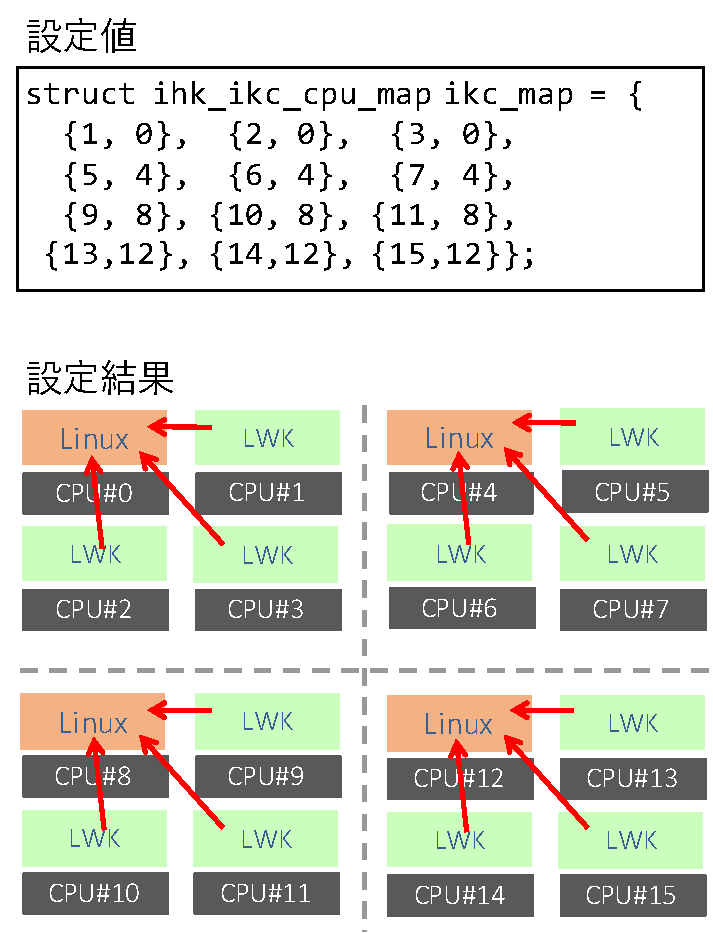
\includegraphics[width=0.5\linewidth]{figs/ikc_map.pdf}
\vspace{-0em}\caption{\texttt{ihk\_os\_set\_ikc\_map()}の例}
\label{fig:ikc_map}
\vspace{-0em}
\end{figure}
\FloatBarrier
%
IKC mapの目的は、IKC通信の送信先CPUを複数にした上で、送信の際に物理的に近いCPUに送るようにすることにより、IKC通信の遅延を削減することである。
\texttt{ihk\_os\_set\_ikc\_map()}の例を図\ref{fig:ikc_map}に示す。
この例では、プロセッサを4つの区画に分け、IKC通信がそれぞれの区画内で閉じるように設定している。

\subsubsection*{戻り値}
\begin{table}[!h]
\footnotesize
\begin{tabular}{|p{0.20\linewidth}|p{0.66\linewidth}|} \hline
0&正常終了\\ \hline
\texttt{-EPERM}&操作に対する権限がない\\ \hline
\texttt{-ENOENT}&指定されたOSインスタンスが存在しない\\ \hline
\texttt{-EINVAL}&不正なパラメータ\\ \hline
\texttt{-EBUSY}&OSインスタンスがブート済みである\\ \hline
\end{tabular}
\vspace{-0em}
\end{table}
\FloatBarrier

\subsubsection{設定リストによるIKC map設定}
\subsubsection*{書式}{\quad} \verb:int ihk_os_set_ikc_map_str(int os_index, const char *envp, int num_env);:
\subsubsection*{説明}{\quad} \verb:os_index:で指定されたOSインスタンスに対し、\verb:envp:と\verb:num_env:で指定された文字列形式の設定リストに従ったIKC map設定を行う。本関数は特権ユーザのみが呼び出せる。

\verb:envp:は\verb:NULL:文字で結合された\verb:num_env:個の設定文字列からなる。各設定文字列は\verb:"KEY=VAL":の形式を持つ。設定可能な項目は以下の通り。
\begin{table}[!h]
\footnotesize
\begin{tabular}{|p{0.30\linewidth}|p{0.65\linewidth}|} \hline
\multicolumn{1}{|c}{\textbf{設定項目}}&\multicolumn{1}{|c|}{\textbf{設定内容}}\\ \hline \hline
\verb:IHK_IKC_MAP=<ikc_map>:&LWKからLinuxへのメッセージの経路を\verb:<ikc_map>:に指定されたものに設定する。\verb:<ikc_map>:の書式は第\ref{sec:ikc_map_cmd}節に記載する。\\ \hline
\end{tabular}
\vspace{-0em}
\end{table}
\\なお、これ以外の設定は無視される。
\FloatBarrier

\subsubsection*{戻り値}
\begin{table}[!h]
\footnotesize
\begin{tabular}{|p{0.15\linewidth}|p{0.80\linewidth}|} \hline
\verb:0:&	成功した\\ \hline
\verb:-EINVAL:&	\verb:envp:の設定値が不正であった\\ \hline
\verb:-ENOMEM:&	メモリ不足が発生した\\ \hline
\verb:-EPERM:&	OSインスタンスを表すデバイスファイルにアクセスできなかった\\ \hline
\verb:-ENOENT:&	OSインスタンスが存在しなかった\\ \hline
\verb:-EFAULT:&	\texttt{envp}にアクセスできなかった\\ \hline
\verb:-EBUSY:&OSインスタンスがブート済みである\\ \hline
\end{tabular}
\vspace{-0em}
\end{table}
\FloatBarrier

\subsubsection{IKC map取得}
\subsubsection*{書式}{\quad} \texttt{int ihk\_os\_get\_ikc\_map(int index, struct ihk\_ikc\_cpu\_map *map, int num\_cpus)}
\subsubsection*{説明}{\quad} \texttt{index}で指定されたOSインスタンスのIKC mapを\texttt{map}で指定された配列に格納する。\texttt{num\_cpus}には配列のサイズを指定する。呼び出し元が\textttw{map}の領域を用意する。なお、この呼び出しは特権ユーザのみ実行できる。

\subsubsection*{戻り値}
\begin{table}[!h]
\footnotesize
\begin{tabular}{|p{0.20\linewidth}|p{0.66\linewidth}|} \hline
0&正常終了\\ \hline
\texttt{-EPERM}&操作に対する権限がない\\ \hline
\texttt{-ENOENT}&指定されたOSインスタンスが存在しない\\ \hline
\texttt{-EINVAL}&不正なパラメータ\\ \hline
\end{tabular}
\vspace{-0em}
\end{table}
\FloatBarrier

\subsubsection{メモリ割当}
\subsubsection*{書式}\begin{tabular}[t]{@{}l@{}}{\quad} \texttt{int ihk\_os\_assign\_mem(int index, struct ihk\_mem\_chunk *mem\_chunks, }\\{\quad}{\quad}\texttt{int num\_mem\_chunks)}\end{tabular}
\subsubsection*{説明}{\quad} \texttt{index}で指定されたOSインスタンスに対し、IHKデバイスに予約されているメモリ領域のうち\texttt{mem\_chunks, num\_mem\_chunks}で指定されたものを割り当てる。\texttt{mem\_chunks}にはメモリ領域情報の配列を指定し、\texttt{num\_mem\_chunks}には配列のサイズを指定する。呼び出し元が\texttt{mem\_chunks}の領域を用意する。この呼び出しは特権ユーザのみ実行できる。\texttt{mem\_chunks}の要素の\texttt{size}フィールドに-1を指定した場合、指定されたNUMAノードについて予約されたメモリ領域の全てを割り当てる。

\subsubsection*{戻り値}
\begin{table}[!h]
\footnotesize
\begin{tabular}{|p{0.20\linewidth}|p{0.66\linewidth}|} \hline
0&正常終了\\ \hline
\texttt{-EPERM}&操作に対する権限がない\\ \hline
\texttt{-ENOENT}&指定されたOSインスタンスが存在しない\\ \hline
\texttt{-EINVAL}&不正なパラメータ\\ \hline
\ADDRCF{\texttt{-EBUSY}}&\ADDRCF{OSインスタンスがブート済みである}\\ \hline
\end{tabular}
\vspace{-0em}
\end{table}
\FloatBarrier

\subsubsection{\ADDJULTWOS{割当済メモリ領域数取得}}
\subsubsection*{書式}{\quad} \texttt{int ihk\_os\_get\_num\_assigned\_mem\_chunks(int index)}
\subsubsection*{説明}{\quad} \texttt{index}で指定されたOSインスタンスに割り当てられているメモリ領域の数を返す。
\subsubsection*{戻り値}
\begin{table}[!h]
\footnotesize
\begin{tabular}{|p{0.20\linewidth}|p{0.66\linewidth}|} \hline
0以上&メモリ領域数\\ \hline
\texttt{-ENOENT}&指定されたOSインスタンスが存在しない\\ \hline
\texttt{-EINVAL}&不正なパラメータ\\ \hline
\end{tabular}
\vspace{-0em}
\end{table}
\FloatBarrier

\subsubsection{\MODAUGS{割当済メモリ領域情報取得}}
\subsubsection*{書式}\begin{tabular}[t]{@{}l@{}}{\quad} \texttt{int ihk\_os\_query\_mem(int index, struct ihk\_mem\_chunks *mem\_chunks, }\\{\quad}{\quad}\texttt{int num\_mem\_chunks)}\end{tabular}
\subsubsection*{説明}{\quad} \texttt{index}で指定されたOSインスタンスに割り当てられているメモリ領域の情報を\texttt{mem\_chunks}に格納する。 \texttt{num\_mem\_chunks}には配列のサイズを指定する。呼び出し元が\texttt{mem\_chunks}の領域を用意する。
\subsubsection*{戻り値}
\begin{table}[!h]
\footnotesize
\begin{tabular}{|p{0.20\linewidth}|p{0.66\linewidth}|} \hline
0&正常終了\\ \hline
\texttt{-ENOENT}&指定されたOSインスタンスが存在しない\\ \hline
\texttt{-EINVAL}&不正なパラメータ\\ \hline
\end{tabular}
\vspace{-0em}
\end{table}
\FloatBarrier

\subsubsection{メモリ領域解放}
\subsubsection*{書式}\begin{tabular}[t]{@{}l@{}}{\quad} \texttt{int ihk\_os\_release\_mem(int index, struct ihk\_mem\_chunks *mem\_chunks, }\\{\quad}{\quad}\texttt{int num\_mem\_chunks)}\end{tabular}
\subsubsection*{説明}{\quad} \texttt{index}で指定されたOSインスタンスに割り当てられているメモリ領域のうち\texttt{mem\_chunks, num\_mem\_chunks}で指定されたものを解放する。\texttt{mem\_chunks}にはメモリ領域情報の配列を指定し、\texttt{num\_mem\_chunks}には配列のサイズを指定する。呼び出し元が\texttt{mem\_chunks}の領域を用意する。\ADDRCF{一連のチャンクの解放の途中で失敗した場合、それまでに解放したチャンクは解放されたままとなる。}この呼び出しは特権ユーザのみ実行できる。\texttt{mem\_chunks}の要素の\texttt{size}フィールドに-1を指定した場合、全てのNUMAノードについて割り当てられたメモリ領域の全てを解放する。

\subsubsection*{戻り値}
\begin{table}[!h]
\footnotesize
\begin{tabular}{|p{0.20\linewidth}|p{0.66\linewidth}|} \hline
0&正常終了\\ \hline
\texttt{-EPERM}&操作に対する権限がない\\ \hline
\texttt{-ENOENT}&指定されたOSインスタンスが存在しない\\ \hline
\texttt{-EINVAL}&不正なパラメータ\\ \hline
\ADDRCF{\texttt{-EBUSY}}&\ADDRCF{OSインスタンスがブート済みである}\\ \hline
\end{tabular}
\vspace{-0em}
\end{table}
\FloatBarrier

\subsubsection{監視用\texttt{eventfd}取得}

\subsubsection*{書式}{\quad} \MODJULTWO{\texttt{int ihk\_os\_get\_eventfd(int index, int type)}}
\subsubsection*{説明}{\quad} \texttt{index}で指定されたOSインスタンスでの\texttt{type}で指定したイベント発生を通知する\texttt{eventfd}を取得する。この呼び出しは特権ユーザのみ実行できる。
%本APIは監視用の\texttt{eventfd}を作成し、IHKドライバに登録した後に\texttt{eventfd}のファイルディスクリプタを返却する。
%\texttt{eventfd}を使用したイベント通知の動作は、Linuxのcgroupメモリサブシステムの\texttt{event\_control}と同様である。
\texttt{type}の取りうる値は以下の通り。
\begin{table}[!h]
\footnotesize
\begin{tabular}{|p{0.10\linewidth}|p{0.85\linewidth}|} \hline
\multicolumn{1}{|c}{\textbf{\texttt{type}の値}}&\multicolumn{1}{|c|}{\textbf{説明}}\\ \hline \hline
0&\DIFFJUL{カーネルおよびユーザのメモリ使用量が(IHKによってLWKに割り当てられた量− 2MiB)を超えた際に通知する。}\\ \hline
2&\MODAUG{OSがハングアップした際またはPANICを起こした際に通知する。}\\ \hline
\end{tabular}
\vspace{-0em}
\end{table}
\FloatBarrier

\begin{figure}[!htb]
\centering
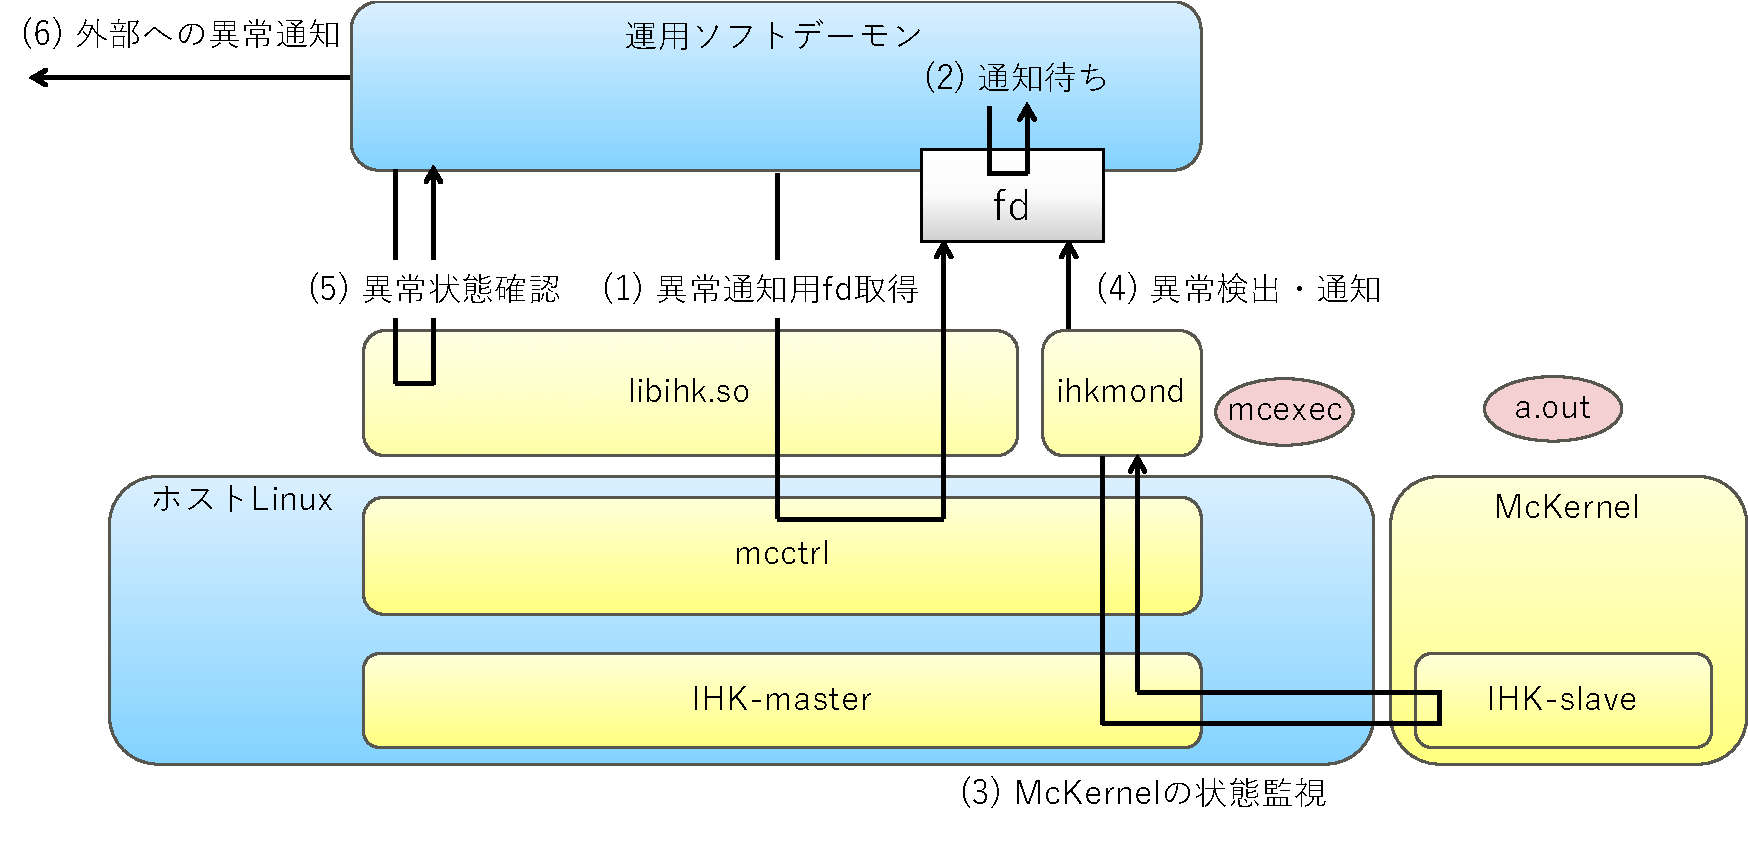
\includegraphics[width=14cm]{figs/monitor.pdf}
\vspace{-0em}\caption{OS状態監視フロー}
\label{fig:monitor}
\vspace{-0em}
\end{figure}
%
\FloatBarrier
%
図\ref{fig:monitor}を用いてLWKとしてMcKernelが動作している場合のOS状態監視のフローを説明する。\texttt{mcctrl}はMcKernelで用いられるカーネルモジュールである。
\begin{enumerate}
\item 運用ソフトデーモンがジョブ実行開始時に\texttt{ihk\_os\_get\_eventfd()}により監視イベント通知用fdを取得する。(図の(1))
\item 運用ソフトデーモンは\texttt{epoll()}などで上記fd経由の通知を待つ。(図の(2))
\item 監視デーモン\texttt{ihkmond}がMcKernelの状態を監視する。(図の(3))なお、McKernelの状態監視機能の詳細は''McKernel Specifications''に記載する。
\item 監視デーモン\texttt{ihkmond}が異常を検出し、上記fd経由でジョブ運用ソフトデーモンに異常を通知する。(図の(4))
\item 運用ソフトデーモンは通知を受けると\texttt{ihk\_os\_get\_status()}によりMcKernelの状態を取得し、実際に異常状態にあることを確認する。(図の(5))
\item 運用ソフトデーモンは確認が取れると外部に異常を通知する。(図の(6))
\end{enumerate}
\FloatBarrier

% \begin{figure}[!htb]
% \centering
% \includegraphics[width=14cm]{figs/hung.pdf}
% \vspace{-0em}\caption{OSハング監視フロー}
% \label{fig:hung}
% \vspace{-0em}
% \end{figure}
% %
% \FloatBarrier
% %
% OSハング監視の動作フローを図\ref{fig:monitor}を用いて説明する。
% \begin{enumerate}
% \item 運用ソフトデーモンがジョブ実行開始時に\texttt{ihk\_os\_get\_eventfd()}により監視イベント通知用FDを取得する。(図上半分の(1))
% \item 運用ソフトデーモンはこのファイルディスクリプタをepollなどで監視する。(図上半分の(2))
% \item McKernelは異常を検出した際にこのFD経由でジョブ運用ソフトデーモンにイベントを通知する。(図下半分の(2))
% \item 運用ソフトデーモンは通知を受けるとMcKernelの状態を取得し、実際に異常状態にあることを確認する。(図下半分の(3))
% \item 運用ソフトデーモンは外部に異常を通知する。(図下半分の(4))
% \end{enumerate}
% \FloatBarrier

\subsubsection*{戻り値}{\quad}
\begin{table}[!h]
\footnotesize
\begin{tabular}{|p{0.20\linewidth}|p{0.66\linewidth}|} \hline
0以上の値&\texttt{eventfd}のファイルデスクリプタ\\ \hline
\texttt{-EPERM}&操作に対する権限がない\\ \hline
\texttt{-ENOENT}&指定されたOSインスタンスが存在しない\\ \hline
\texttt{-EINVAL}&不正なパラメータ\\ \hline
\end{tabular}
\vspace{-0em}
\end{table}
\FloatBarrier

\subsubsection{カーネルロード}
\subsubsection*{書式}{\quad} \texttt{int ihk\_os\_load(int index, char *image)}
\subsubsection*{説明}{\quad} \texttt{index}で指定されたOSインスタンスに\texttt{image}で指定されたファイル名のカーネルイメージをロードする。なお、ポスト京ではOSインスタンスは1つのみ生成するため、OSインデックスは0を固定的に指定してよい。この呼び出しは特権ユーザのみ実行できる。

\subsubsection*{戻り値}
\begin{table}[!h]
\footnotesize
\begin{tabular}{|p{0.20\linewidth}|p{0.66\linewidth}|} \hline
0&正常終了\\ \hline
\texttt{-EPERM}&操作に対する権限がない\\ \hline
\texttt{-ENOENT}&指定されたOSインスタンスが存在しない\\ \hline
\texttt{-EINVAL}&\MODRCF{イメージがロードできない、割当メモリまたは割当CPUが不足している}\\ \hline
\ADDRCF{\texttt{-EBUSY}}&\ADDRCF{OSインスタンスがブート済みである}\\ \hline
\end{tabular}
\vspace{-0em}
\end{table}
\FloatBarrier

\subsubsection{カーネル引数設定}
\subsubsection*{書式}{\quad} \texttt{int ihk\_os\_kargs(int index, char *kargs)}
\subsubsection*{説明}{\quad} \texttt{index}で指定されたOSインスタンスに\texttt{kargs}に格納されているカーネル引数を渡す。この呼び出しは特権ユーザのみ実行できる。なお、\verb:hidos:の文字列を含まない場合は\verb:-EINVAL:を返す。

\subsubsection*{戻り値}
\begin{table}[!h]
\footnotesize
\begin{tabular}{|p{0.15\linewidth}|p{0.80\linewidth}|} \hline
0&正常終了\\ \hline
\texttt{-EPERM}&操作に対する権限がない\\ \hline
\texttt{-ENOENT}&指定されたOSインスタンスが存在しない\\ \hline
\texttt{-EINVAL}&不正なパラメータ\\ \hline
\ADDRCF{\texttt{-EBUSY}}&\ADDRCF{OSインスタンスがブート済みである}\\ \hline
\ADDRCF{\texttt{-EFAULT}}&\ADDRCF{\texttt{kargs}にアクセスできない}\\ \hline
\end{tabular}
\vspace{-0em}
\end{table}
\FloatBarrier

\subsubsection{設定リストによるカーネル引数設定}
\subsubsection*{書式}{\quad} \verb:int ihk_os_kargs_str(int os_index, const char *envp, int num_env,:\\ \quad\quad
\verb:const char *default_kargs);:
\subsubsection*{説明}{\quad} \verb:os_index:で指定されたOSインスタンスに対し、\verb:envp:と\verb:num_env:で指定された文字列形式の設定リストに従ってOSインスタンスのカーネル引数を設定する。なお、\verb:envp:に指定がなかった場合は、\verb:default_kargs:に格納された内容を用いる。本関数は特権ユーザのみが呼び出せる。

\verb:envp:は\verb:NULL:文字で結合された\verb:num_env:個の設定文字列からなる。各設定文字列は\verb:"KEY=VAL":の形式を持つ。設定可能な項目は以下の通り。
\begin{table}[!h]
\footnotesize
\begin{tabular}{|p{0.30\linewidth}|p{0.65\linewidth}|} \hline
\multicolumn{1}{|c}{\textbf{設定項目}}&\multicolumn{1}{|c|}{\textbf{設定内容}}\\ \hline \hline
\verb:IHK_KARGS=<kargs>:&\verb:<kargs>:をカーネル引数としてLWKに渡す。\\ \hline
\end{tabular}
\vspace{-0em}
\end{table}
\\なお、これ以外の設定は無視される。
\FloatBarrier

\subsubsection*{戻り値}
\begin{table}[!h]
\footnotesize
\begin{tabular}{|p{0.15\linewidth}|p{0.80\linewidth}|} \hline
\verb:0:&	成功した\\ \hline
\verb:-EINVAL:&	\verb:envp:の設定値が不正であった\\ \hline
\verb:-ENOMEM:&	メモリ不足が発生した\\ \hline
\verb:-EPERM:&	OSインスタンスを表すデバイスファイルにアクセスできなかった\\ \hline
\verb:-ENOENT:&	OSインスタンスが存在しなかった\\ \hline
\verb:-EFAULT:&	\verb:envp:または\verb:default_kargs:にアクセスできなかった\\ \hline
\verb:-EBUSY:&OSインスタンスがブート済みである\\ \hline
\end{tabular}
\vspace{-0em}
\end{table}
\FloatBarrier

\subsubsection{(廃止予定)設定リストによるOSインスタンスの作成と設定}
\subsubsection*{書式}{\quad} \verb:int ihk_create_os_str(int dev_index, int *os_index,:\\{\quad}{\quad}
\verb:const char *env_p, int num_env, const char *kernel_image,:\\{\quad}{\quad}
\verb:const char *default_kargs, char *err_msg);:
\subsubsection*{説明}{\quad} \verb:dev_index:で指定されたIHKデバイスに対し、\verb:envp:と\verb:num_env:で指定された設定リストに従って、OSインスタンスの作成と設定とを行う。本関数は特権ユーザのみが呼び出せる。

ステップは以下の通り。
\begin{enumerate}
\item 資源を予約する。なお、資源が既に予約されていた場合は全ての資源を解放してから予約を行う。
\item OSインスタンスを作成する。インデックスは\verb:os_index:に格納される。
\item OSインスタンスに予約した資源全てを割り当てる
\item LWKからLinuxへのメッセージの経路を設定する
\item \verb:kernel_image:で指定されたカーネルイメージをロードする
\item OSインスタンスのカーネル引数を設定する。なお、\verb:envp:に指定がなかった場合は、\verb:default_kargs:に格納された内容を用いる。
\end{enumerate}

\verb:envp:は\verb:NULL:文字で結合された\verb:num_env:個の設定文字列からなる。各設定文字列は\verb:"KEY=VAL":の形式を持つ。設定可能な項目は以下の通り。なお、「必須」と記された項目がない場合は、本関数は-EINVALを返す。また、これ以外の設定は無視される。
\begin{table}[!h]
\footnotesize
\begin{tabular}{|p{0.65\linewidth}|p{0.30\linewidth}|} \hline
\multicolumn{1}{|c}{\textbf{設定項目}}&\multicolumn{1}{|c|}{\textbf{設定内容}}\\ \hline \hline
\verb:IHK_CPUS=<cpus>: (必須)&\verb:<cpus>:に指定されたCPUをMcKernelに割り当てる。\verb:<cpus>:の書式は第\ref{sec:reserve_cpu}節に記載する。\\ \hline
\verb:IHK_RESERVE_MEM_BALANCED_ENABLE=(0|1):&\multirow{6}{\linewidth}{それぞれ、第\ref{sec:balanced}節に記載のメモリ予約の動作設定について、左辺のKeyに対する値を右辺の値に設定する。}\\
\verb:IHK_RESERVE_MEM_BALANCED_BEST_EFFORT=(0|1):&\\
\verb:IHK_RESERVE_MEM_BALANCED_VARIANCE_LIMIT=<limit_in_%>:&\\
\verb:IHK_RESERVE_MEM_MIN_CHUNK_SIZE=<size>:&\\
\verb:IHK_RESERVE_MEM_MAX_SIZE_RATIO_ALL=<cap_in_%>:&\\
\verb:IHK_RESERVE_MEM_MEM_TIMEOUT=<timeout_in_second>:&\\ \hline
\verb:IHK_MEM=<mems>: (必須)&\verb:<mems>:に指定されたメモリをMcKernelに割り当てる。\verb:<mems>:の書式は第\ref{sec:reserve_mem}節に記載する。\\ \hline
\verb:IHK_IKC_MAP=<ikc_map>:&LWKからLinuxへのメッセージの経路を\verb:<ikc_map>:に指定されたものに設定する。\verb:<ikc_map>:の書式は第\ref{sec:ikc_map_cmd}節に記載する。\\ \hline
\verb:IHK_KARGS=<kargs>:&\verb:<kargs>:をカーネル引数としてLWKに渡す。\\ \hline
\end{tabular}
\vspace{-0em}
\end{table}
\FloatBarrier

本関数は、エラー発生時は、OSインスタンスは全て削除された状態で、またCPUおよびメモリは全て解放された状態で復帰する。本関数内でのIHKインターフェイス関数の呼び出しでエラーが発生した場合は、\verb:err_msg:にエラーメッセージが書き込まれる。書き込まれる内容には、呼び出し元のソースコードの名前と行番号、エラーを起こした関数の名前が含まれる。なお、本関数の呼び出し元が\verb:err_msg:の領域を用意する。


\subsubsection*{戻り値}
\begin{table}[!h]
\footnotesize
\begin{tabular}{|p{0.15\linewidth}|p{0.80\linewidth}|} \hline
\verb:0:&	成功した\\ \hline
\verb:-EINVAL:&	\verb:envp:の内容が適切でなかった。具体的には、必須の設定がなかった、あるいは設定値が不正であった。\\ \hline
\verb:-ENOMEM:&	メモリ不足が発生した\\ \hline
\verb:-EPERM:&	IHKデバイスを表すデバイスファイルまたはOSインスタンスを表すデバイスファイルにアクセスできなかった\\ \hline
\verb:-ENOENT:&	IHKデバイスまたはOSインスタンスが存在しなかった\\ \hline
\verb:-EFAULT:&	関数内部で使用する一時バッファにアクセスできなかった\\ \hline
\end{tabular}
\vspace{-0em}
\end{table}
\FloatBarrier

\subsubsection{ブート}
\subsubsection*{書式}{\quad} \texttt{int ihk\_os\_boot(int index)}
\subsubsection*{説明}{\quad} \texttt{index}で指定されたOSインスタンスのカーネルをブートする。この呼び出しは特権ユーザのみ実行できる。

\subsubsection*{戻り値}
\begin{table}[!h]
\footnotesize
\begin{tabular}{|p{0.20\linewidth}|p{0.66\linewidth}|} \hline
0&正常終了\\ \hline
\texttt{-EPERM}&操作に対する権限がない\\ \hline
\texttt{-ENOENT}&指定されたOSインスタンスが存在しない\\ \hline
\texttt{-EINVAL}&不正なパラメータ\\ \hline
\end{tabular}
\vspace{-0em}
\end{table}
\FloatBarrier

\subsubsection{シャットダウン}
\subsubsection*{書式}{\quad} \texttt{int ihk\_os\_shutdown(int index)}
\subsubsection*{説明}{\quad} \texttt{index}で指定されたOSインスタンスのカーネルをシャットダウンする。\ADDJULTWO{当該OSインスタンスに割り当てられた資源は解放される。}\MODRCF{この関数はOSの状態が\texttt{IHK\_STATUS\_INACTIVE}に遷移したことを確認せずに復帰する。}操作完了は\texttt{ihk\_os\_get\_status}で確認できる。なお、OSインスタンスが既にシャットダウン中である場合は何も行わず、ゼロを返す。この呼び出しは特権ユーザのみ実行できる。

\subsubsection*{戻り値}
\begin{table}[!h]
\footnotesize
\begin{tabular}{|p{0.20\linewidth}|p{0.66\linewidth}|} \hline
0&シャットダウンに成功、または既にシャットダウン済\\ \hline
\texttt{-EPERM}&操作に対する権限がない\\ \hline
\texttt{-ENOENT}&指定されたOSインスタンスが存在しない\\ \hline
\texttt{-EINVAL}&\MODRCF{OSインスタンスがブート前である}\\ \hline
\end{tabular}
\vspace{-0em}
\end{table}
\FloatBarrier

\subsubsection{\ADDJULTWOS{OS状態取得}}
\subsubsection*{書式}{\quad} \texttt{int ihk\_os\_get\_status(int index)}
\subsubsection*{説明}{\quad} \texttt{index}で指定されたOSインスタンスの状態を返す。

OSの状態は\texttt{enum ihklib\_os\_status}で表される。
\texttt{enum ihklib\_os\_status}は以下のように定義される。
\small
\begin{verbatim}
enum ihklib_os_status {
    IHK_STATUS_INACTIVE, // 起動前
    IHK_STATUS_BOOTING,  // 起動中
    IHK_STATUS_RUNNING,  // 起動後
    IHK_STATUS_SHUTDOWN, // シャットダウン中
    IHK_STATUS_PANIC,    // PANIC
    IHK_STATUS_HUNGUP,   // ハングアップ
    IHK_STATUS_FREEZING, // 一時停止状態へ移行中
    IHK_STATUS_FROZEN,   // 一時停止状態
};
\end{verbatim}
\normalsize
%なお、\texttt{IHK\_STATUS\_RUNNING}の状態では、IKC Channelは確立しており、/sysファイルシステムの準備も完了しているため、IKCを必要としたり、/sysファイルシステム準備完了を前提としたりする関数(例:\texttt{ihk_os_setperfevent()}、\texttt{ihk_os_shutdown()})を安全に呼び出すことができる。

\subsubsection*{戻り値}
\begin{table}[!h]
\footnotesize
\begin{tabular}{|p{0.20\linewidth}|p{0.66\linewidth}|} \hline
0以上&OS状態\\ \hline
\texttt{-ENOENT}&指定されたOSインスタンスが存在しない\\ \hline
\texttt{-EINVAL}&不正なパラメータ\\ \hline
\end{tabular}
\vspace{-0em}
\end{table}
\FloatBarrier

\subsubsection{カーネルメッセージサイズ取得}
\subsubsection*{書式}{\quad} \texttt{ssize\_t ihk\_os\_get\_kmsg\_size(int index)}
\subsubsection*{説明}{\quad} \texttt{index}で指定されたOSインスタンスのカーネルメッセージ用バッファのサイズを返す。

\subsubsection*{戻り値}
\begin{table}[!h]
\footnotesize
\begin{tabular}{|p{0.20\linewidth}|p{0.66\linewidth}|} \hline
正の値&カーネルメッセージのサイズ\\ \hline
\texttt{-ENOENT}&指定されたOSインスタンスが存在しない\\ \hline
\texttt{-EINVAL}&不正なパラメータ\\ \hline
\end{tabular}
\vspace{-0em}
\end{table}
\FloatBarrier

\subsubsection{カーネルメッセージ取得}
\subsubsection*{書式}{\quad} \texttt{int ihk\_os\_kmsg(int index, char *kmsg, size\_t size\_kmsg)}
\subsubsection*{説明}{\quad} \texttt{index}で指定されたOSインスタンスのカーネルメッセージを\texttt{kmsg}にコピーする。\texttt{size\_kmsg}の値は\texttt{ihk\_os\_get\_kmsg\_size}が返す値と等しい必要がある。なお、呼び出し元が\texttt{kmsg}の領域を用意する。

\subsubsection*{戻り値}
\begin{table}[!h]
\footnotesize
\begin{tabular}{|p{0.20\linewidth}|p{0.66\linewidth}|} \hline
\MODAUG{0以上の値}&\MODAUG{コピーしたバイト数}\\ \hline
\texttt{-ENOENT}&指定されたOSインスタンスが存在しない\\ \hline
\texttt{-EINVAL}&不正なパラメータ\\ \hline
\end{tabular}
\vspace{-0em}
\end{table}
\FloatBarrier

\subsubsection{\ADDJULTWOS{カーネルメッセージクリア}}
\subsubsection*{書式}{\quad} \texttt{int ihk\_os\_clear\_kmsg(int index)}
\subsubsection*{説明}{\quad} \texttt{index}で指定されたOSインスタンスのカーネルメッセージをクリアする。

\subsubsection*{戻り値}
\begin{table}[!h]
\footnotesize
\begin{tabular}{|p{0.20\linewidth}|p{0.66\linewidth}|} \hline
0&正常終了\\ \hline
\texttt{-ENOENT}&指定されたOSインスタンスが存在しない\\ \hline
\texttt{-EINVAL}&不正なパラメータ\\ \hline
\end{tabular}
\vspace{-0em}
\end{table}
\FloatBarrier

\subsubsection{\ADDJULTWOS{NUMAノード数取得}}
\subsubsection*{書式}{\quad} \texttt{int ihk\_os\_get\_num\_numa\_nodes(int index)}
\subsubsection*{説明}{\quad} \texttt{index}で指定されたOSインスタンスが利用可能なNUMAノードの数を返す。
\subsubsection*{戻り値}
\begin{table}[!h]
\footnotesize
\begin{tabular}{|p{0.20\linewidth}|p{0.66\linewidth}|} \hline
1以上&NUMAノード数\\ \hline
0&エラー\\ \hline
\end{tabular}
\vspace{-0em}
\end{table}
\FloatBarrier

\subsubsection{\MODAUGS{空きメモリ量取得}}
\subsubsection*{書式}{\quad} \texttt{int ihk\_os\_query\_free\_mem(int index, unsigned long *memfree, int num\_numa\_nodes)}
\subsubsection*{説明}{\quad} \MODJULTWO{\texttt{index}で指定されたOSインスタンスのNUMAノードごとの空きメモリ量を\texttt{memfree}で指定された配列に格納する。 \texttt{num\_numa\_nodes}には配列のサイズを指定する。}呼び出し元が\texttt{memfree}の領域を用意する。
\subsubsection*{戻り値}
\begin{table}[!h]
\footnotesize
\begin{tabular}{|p{0.20\linewidth}|p{0.66\linewidth}|} \hline
0&正常終了\\ \hline
\texttt{-ENOENT}&指定されたOSインスタンスが存在しない\\ \hline
\texttt{-EINVAL}&不正なパラメータ\\ \hline
\end{tabular}
\vspace{-0em}
\end{table}
\FloatBarrier
 
\subsubsection{ページサイズ種数取得}
\subsubsection*{書式}{\quad} \texttt{int ihk\_os\_get\_num\_pagesizes(int index)}
\subsubsection*{説明}{\quad} \texttt{index}で指定されたOSインスタンスのページサイズ種数を返す。
\texttt{ihk\_os\_get\_pagesizes()}と組み合わせることでページサイズの表を取得できる。

\subsubsection*{戻り値}
\begin{table}[!h]
\footnotesize
\begin{tabular}{|p{0.20\linewidth}|p{0.66\linewidth}|} \hline
1以上&ページサイズ種数\\ \hline
0&エラー\\ \hline
\end{tabular}
\vspace{-0em}
\end{table}
\FloatBarrier

\subsubsection{ページサイズ取得}
\subsubsection*{書式}{\quad} \texttt{int ihk\_os\_get\_pagesizes(int index, long *pgsizes, int num\_pgsizes)}
\subsubsection*{説明}{\quad} \texttt{index}で指定されたOSインスタンスのページサイズ表を\texttt{pgsizes}で指定された配列に格納する。\texttt{num\_pgsizes}には配列のサイズを指定する。呼び出し元が\texttt{pgsizes}の領域を用意する。なお、ページサイズ表には、LWKで利用できるページサイズ以外のページサイズが含まれることがある。
\subsubsection*{戻り値}
\begin{table}[!h]
\footnotesize
\begin{tabular}{|p{0.20\linewidth}|p{0.66\linewidth}|} \hline
0&正常終了\\ \hline
\texttt{-ENOENT}&指定されたOSインスタンスが存在しない\\ \hline
\texttt{-EINVAL}&不正なパラメータ\\ \hline
\end{tabular}
\vspace{-0em}
\end{table}
\FloatBarrier

\subsubsection{統計情報取得}
\subsubsection*{書式}{\quad} \texttt{int ihk\_os\_getrusage(int index, struct ihk\_os\_rusage *rusage)}
\subsubsection*{説明}{\quad} \texttt{index}で指定されたOSインスタンスの呼び出し時点での統計情報を\texttt{rusage}に格納する。呼び出し元が\texttt{rusage}の領域を用意する。

\texttt{struct ihk\_os\_rusage}型は以下のように定義される。なお、\verb|cpuacct_usage_percpu|のインデックスはLWKでのCPU番号である。

\footnotesize
\begin{Verbatim}[commandchars=\\\{\}]
struct ihk_os_rusage \{
    unsigned long memory_stat_rss[IHK_MAX_NUM_PGSIZES];
    /* ユーザのぺージサイズごとのanonymousページ使用量現在値(バイト単位) */
    unsigned long memory_stat_mapped_file[IHK_MAX_NUM_PGSIZES];
    /* ユーザのページサイズごとのfile-backedページ使用量現在値(バイト単位) */
    unsigned long memory_max_usage;
    /* ユーザのメモリ使用量最大値(バイト単位) */
    unsigned long memory_kmem_usage;
    /* カーネルのメモリ使用量現在値(バイト単位) */
    unsigned long memory_kmem_max_usage;
    /* カーネルのメモリ使用量最大値(バイト単位) */
    unsigned long memory_numa_stat[IHK_MAX_NUM_NUMA_NODES];
    /* NUMAごとのユーザのメモリ使用量現在値(バイト単位) */
    unsigned long cpuacct_stat_system;
    /* システム時間(USER_HZ単位) */
    unsigned long cpuacct_stat_user;
    /* ユーザ時間(USER_HZ単位) */
    unsigned long cpuacct_usage;
    /* ユーザのCPU時間(ナノ秒単位) */
    unsigned long cpuacct_usage_percpu[IHK_MAX_NUM_CPUS];
    /* コアごとのユーザのCPU時間(ナノ秒単位)*/
    int num_threads;
    /* スレッド数現在値 */
    int max_num_threads;
    /* スレッド数最大値 */
\};
\end{Verbatim}
\normalsize

\texttt{memory\_stat\_rss}および\texttt{memory\_stat\_mapped\_file}のインデックスはサイズによるページ種であり、以下のように定義される。
\footnotesize
\begin{Verbatim}[commandchars=\\\{\}]
enum ihk_os_pgsize \{
        IHK_OS_PGSIZE_4KB,
        IHK_OS_PGSIZE_64KB,
        IHK_OS_PGSIZE_2MB,
        IHK_OS_PGSIZE_32MB,
        IHK_OS_PGSIZE_1GB,
        IHK_OS_PGSIZE_16GB,
        IHK_OS_PGSIZE_512MB,
        IHK_OS_PGSIZE_4TB,
        IHK_MAX_NUM_PGSIZES
\};
\end{Verbatim}
\normalsize

\subsubsection*{戻り値}{\quad}
\begin{table}[!h]
\footnotesize
\begin{tabular}{|p{0.20\linewidth}|p{0.66\linewidth}|} \hline
0&正常終了\\ \hline
\texttt{-ENOENT}&指定されたOSインスタンスが存在しない\\ \hline
\texttt{-EINVAL}&不正なパラメータ\\ \hline
\end{tabular}
\vspace{-0em}
\end{table}
\FloatBarrier

\subsubsection{CPU PA情報採取イベント登録}
\subsubsection*{書式}{\quad} \MODJULTWO{\texttt{int ihk\_os\_setperfevent(int index, struct ihk\_perf\_event\_attr attr[], int n)}}
\subsubsection*{説明}{\quad} 
\texttt{index}で指定されたOSインスタンスにおいて\texttt{attr, n}で指定したイベントを収集する設定を行う。
\texttt{n}はイベント種数で、ハードウェアが備えるPAカウンタ数以下の値を指定する。
呼び出し元が\texttt{attr}の領域を用意する。この関数は特権ユーザのみ呼び出せる。

\texttt{ihk\_perf\_event\_attr}は以下のように定義される。
%なお、本構造体は\texttt{perf\_event\_attr}構造体に似た構造を持つ。
\footnotesize
\begin{Verbatim}[obeytabs]
struct ihk_perf_event_attr{
    unsigned long config;      // ハードウェアで規定されるイベント番号
    unsigned disabled:1;       // 無効設定
    unsigned pinned:1;         // 常に収集対象とする
    unsigned exclude_user:1;   // ユーザモードで発生したイベントを計上しない
    unsigned exclude_kernel:1; // カーネルモードで発生したイベントを計上しない
    unsigned exclude_hv:1;     // hypervisorモードで発生したイベントを計上しない
    unsigned exclude_idle:1;   // idle状態のイベントを計上しない
};
\end{Verbatim}
\normalsize

\begin{figure}[!htb]
\centering
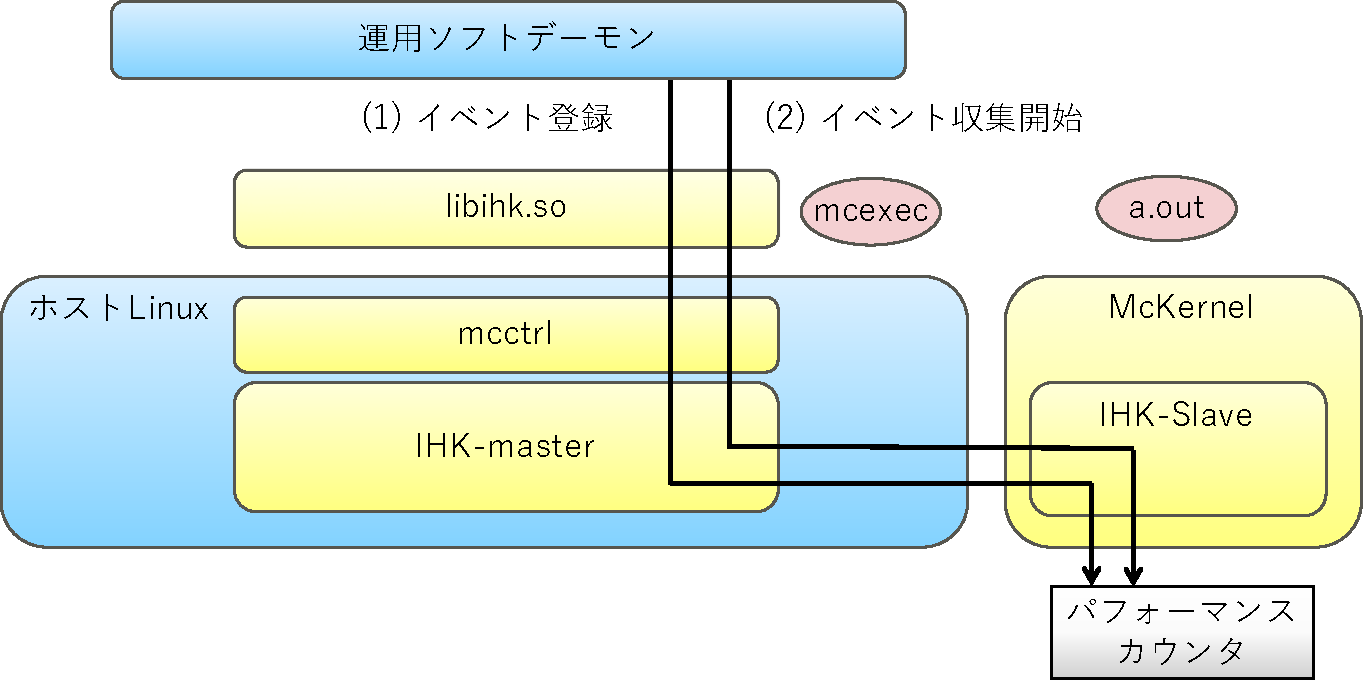
\includegraphics[width=12cm]{figs/cpupa_sow.pdf}
\vspace{-0em}\caption{CPU PA情報の収集開始のフロー}
\label{fig:cpupa_sow}
\vspace{-0em}
\end{figure}
%
\FloatBarrier
%
CPU PA情報の収集は運用ソフトデーモンによって行われる。
運用ソフトデーモンはジョブプロセス開始直前に収集を開始し、ジョブプロセス終了直後に収集を停止し値を回収する。
図\ref{fig:cpupa_sow}を用いてLWKとしてMcKernelが動作している際の収集開始のフローを説明する。
\begin{enumerate}
\item 運用ソフトデーモンが\texttt{ihk\_os\_setperfevent()}を用いて取得するCPU PA情報(イベント)の設定を行う。(図の(1))
\item 運用ソフトデーモンが\texttt{ihk\_os\_perfctl()}を用いてイベント収集を開始する。(図の(2))
\end{enumerate}

\begin{figure}[!htb]
\centering
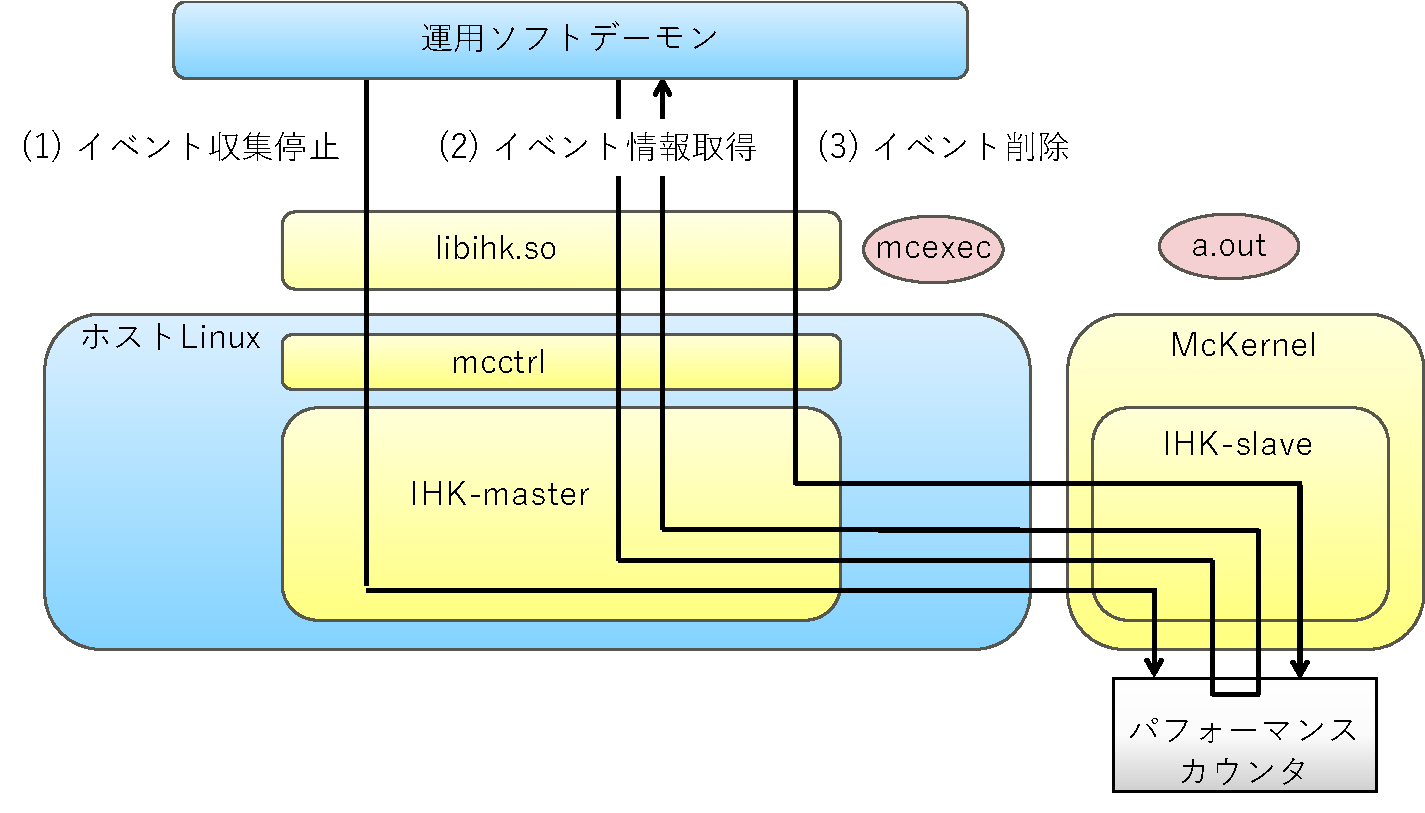
\includegraphics[width=12cm]{figs/cpupa_reap.pdf}
\vspace{-0em}\caption{CPU PA情報の収集停止と値回収のフロー}
\label{fig:cpupa_reap}
\vspace{-0em}
\end{figure}
%
\FloatBarrier
%
図\ref{fig:cpupa_reap}を用いて収集停止と値回収のフローを説明する。
\begin{enumerate}
\item 運用ソフトデーモンが\texttt{ihk\_os\_perfctl()}を用いてイベント収集を停止する。(図の(1))
\item 運用ソフトデーモンが\texttt{ihk\_os\_getperfevent()}を用いてCPU PA情報の取得(値の読み出し)を行う。(図の(2))
\item 運用ソフトデーモンが\texttt{ihk\_os\_perfctl()}を用いてイベントを削除する。(図の(3))
\end{enumerate}


\subsubsection*{戻り値}{\quad}
\begin{table}[!h]
\footnotesize
\begin{tabular}{|p{0.20\linewidth}|p{0.66\linewidth}|} \hline
0または正の値&正常終了。登録に成功したイベント数を返す。\\ \hline
\texttt{-EPERM}&操作に対する権限がない\\ \hline
\texttt{-ENOENT}&指定されたOSインスタンスが存在しない\\ \hline
\texttt{-EINVAL}&\MODRCF{不正なパラメタ、またはOSインスタンスが起動していない}\\ \hline
\end{tabular}
\vspace{-0em}
\end{table}
\FloatBarrier

\subsubsection{CPU PA情報収集開始停止}
\subsubsection*{書式}{\quad} \MODJULTWOS{\texttt{int ihk\_os\_perfctl(int index, int comm)}}
\subsubsection*{説明}{\quad} 
\texttt{index}で指定されたOSインスタンスに対して\texttt{comm}で指定するサブコマンドを用いてPAイベント収集の制御を行う。この関数は特権ユーザのみ呼び出せる。

サブコマンドには以下の値を指定する。 
\begin{table}[!h]
\footnotesize
\begin{tabular}{|p{0.20\linewidth}|p{0.20\linewidth}|p{0.45\linewidth}|} \hline
\multicolumn{1}{|c}{\textbf{値(マクロ)}}&\multicolumn{1}{|c}{\textbf{コマンドの意味}}&\multicolumn{1}{|c|}{\textbf{運用ソフトでの使用タイミング}}\\ \hline \hline
\texttt{PERF\_EVENT\_ENABLE} &PAイベント収集開始 &ジョブ開始時に使用\\ \hline 
\texttt{PERF\_EVENT\_DISABLE} &PAイベント収集停止 &ジョブ終了時に使用\\ \hline 
\texttt{PERF\_EVENT\_DESTROY} &PAイベント削除 &ジョブ終了時に使用   \\ \hline 
\end{tabular}
\vspace{-0em}
\end{table}
\FloatBarrier


\subsubsection*{戻り値}{\quad}
\begin{table}[!h]
\footnotesize
\begin{tabular}{|p{0.20\linewidth}|p{0.66\linewidth}|} \hline
0&正常終了\\ \hline
\texttt{-EPERM}&操作に対する権限がない\\ \hline
\texttt{-ENOENT} &indexで指定されたOSインスタンスが存在しない\\ \hline
\texttt{-EINVAL}&不正なパラメタ\\ \hline
\end{tabular}
\vspace{-0em}
\end{table}
\FloatBarrier

\subsubsection{\MODAUGS{CPU PA情報取得}}
\subsubsection*{書式}{\quad} \MODJULTWO{\texttt{int ihk\_os\_getperfevent(int index, unsigned long *counter, int n)}}
\subsubsection*{説明}{\quad} 
\texttt{index}で指定されたOSインスタンスのイベント発生回数を要素数\texttt{n}の配列\texttt{counter}に格納する。
\texttt{n}はイベント種数で、\texttt{ihk\_os\_setperfevent}の戻り値、すなわち登録に成功したイベント種数を指定する。
呼び出し元が\texttt{counter}の領域を用意する。
この関数は特権ユーザのみ呼び出せる。

\subsubsection*{戻り値}{\quad}
\begin{table}[!h]
\footnotesize
\begin{tabular}{|p{0.20\linewidth}|p{0.66\linewidth}|} \hline
0&正常終了\\ \hline
\texttt{-ENOENT}&indexで指定されたOSインスタンスが存在しない\\ \hline
\texttt{-EINVAL}&不正なパラメタ\\ \hline
\end{tabular}
\vspace{-0em}
\end{table}
\FloatBarrier

\subsubsection{全CPU一時停止}
\subsubsection*{書式}{\quad} \MODJULTWOS{\texttt{int ihk\_os\_freeze(unsigned long *os\_set, int n)}}
\subsubsection*{説明}{\quad} 
\texttt{os\_set}で指定されたOSインスタンスについて、全CPUの一時停止状態への遷移を開始して即座に復帰する。対象OSインスタンスの状態は、1以上CPU数未満の数のCPUが一時停止状態へ遷移した時に\texttt{IHK\_STATUS\_FREEZING}に遷移し、全CPUが一時停止状態へ遷移した時に\texttt{IHK\_STATUS\_FROZEN}に遷移する。操作が一定時間で完了しないケースは\texttt{ihk\_os\_get\_status()}を用いて検出することができる。この場合は\texttt{ihk\_os\_thaw()}を用いて遷移をキャンセルすることができる。\texttt{os\_set}は長さnのビット列を指すポインタで、LSBから数えて第$i$番目のビットが1の場合はOSインデックスが$i$であるOSインスタンスが操作の対象となる。なお、この関数は特権ユーザのみ呼び出せる。

\begin{figure}[!htb]
\centering
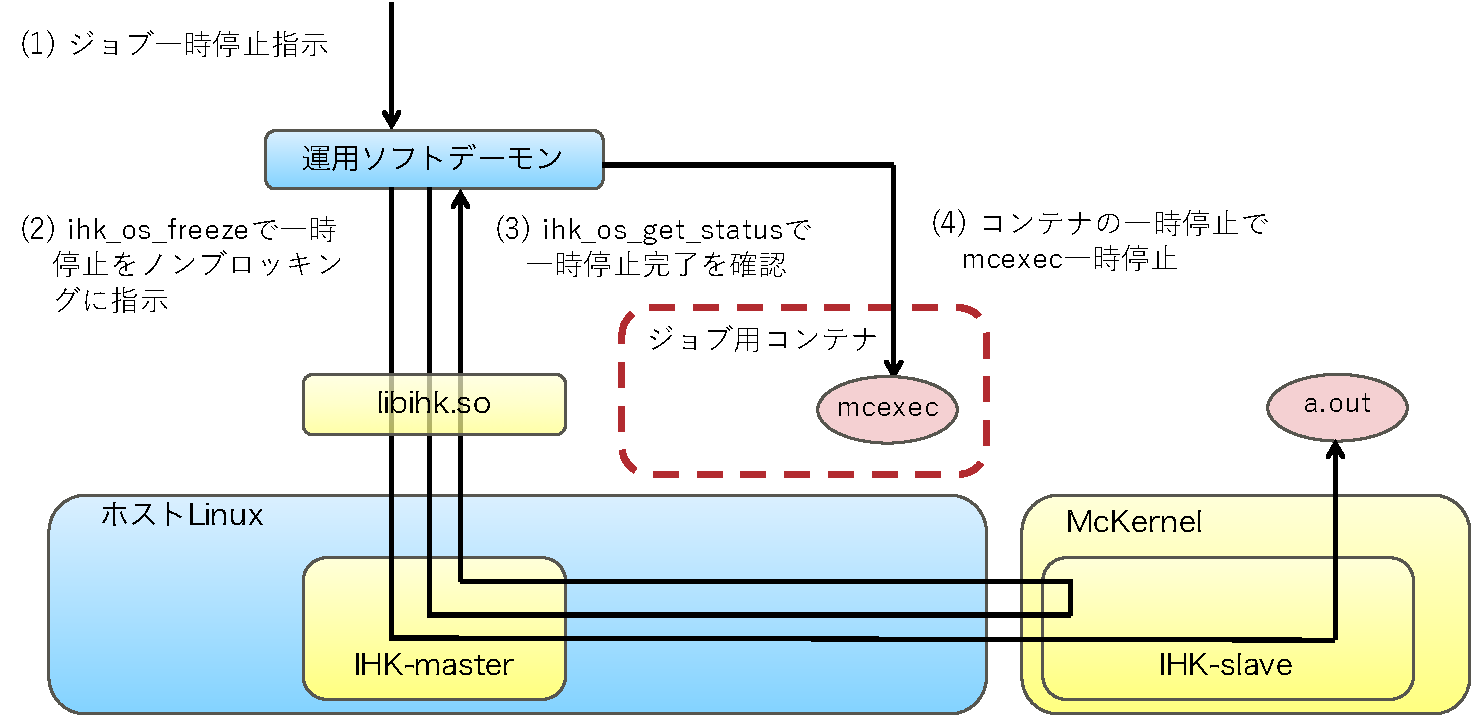
\includegraphics[width=14cm]{figs/freeze.pdf}
\vspace{-0em}\caption{全CPU一時停止のフロー}
\label{fig:freeze}
\vspace{-0em}
\end{figure}
%
全CPU一時停止の動作フローを図\ref{fig:freeze}を用いて説明する。
\begin{enumerate}
\item 運用ソフトがノードの運用ソフトデーモンにジョブの一時停止を指示する。(図の(1))
\item 運用ソフトデーモンが\texttt{ihk\_os\_freeze()}でMcKernelに全CPUの一時停止をノンブロッキングに指示する。(図の(2))
\item 運用ソフトデーモンが\texttt{ihk\_os\_get\_status()}で全CPUの一時停止の完了を確認する。(図の(3))
\item 運用ソフトデーモンがコンテナの状態を変えることでmcexec (proxy process)を一時停止状態にする。(図の(4))
\end{enumerate}
%
\FloatBarrier

\subsubsection*{戻り値}{\quad}
\begin{table}[!h]
\footnotesize
\begin{tabular}{|p{0.20\linewidth}|p{0.66\linewidth}|} \hline
0&正常終了\\ \hline
\ADDAUG{-EINVAL}&\begin{tabular}[t]{@{}l@{}}OSインスタンスのステータスが\\\texttt{IHK\_STATUS\_RUNNING}、\texttt{IHK\_STATUS\_FREEZING}、\texttt{IHK\_STATUS\_FROZEN}以外\end{tabular}\\ \hline
\ADDRCF{-EBUSY}&\ADDRCF{OSインスタンスのステータスが\texttt{IHK\_STATUS\_FREEZING}または\texttt{IHK\_STATUS\_FROZEN}}\\ \hline
\texttt{-EPERM}&操作に対する権限がない\\ \hline
\MODAUG{\texttt{-ENOENT}}&indexが示すOSインスタンスは存在しない\\ \hline
\end{tabular}
\vspace{-0em}
\end{table}
\FloatBarrier

\subsubsection{全CPU一時停止からの復帰}
\subsubsection*{書式}{\quad} \MODJULTWOS{\texttt{int ihk\_os\_thaw(unsigned long *os\_set, int n)}}
\subsubsection*{説明}{\quad} 
\MODAUG{\texttt{os\_set}で指定されたOSインスタンスについて、一時停止状態にあるか、一時停止状態へ遷移しつつあるCPUを元の状態に戻す。}また、OSの状態を\texttt{IHK\_STATUS\_RUNNING}にする。\texttt{os\_set}は長さnのビット列を指すポインタで、LSBから数えて第$i$番目のビットが1の場合はOSインデックスが$i$であるOSインスタンスが操作の対象となる。なお、この関数は特権ユーザのみ呼び出せる。

\begin{figure}[!htb]
\centering
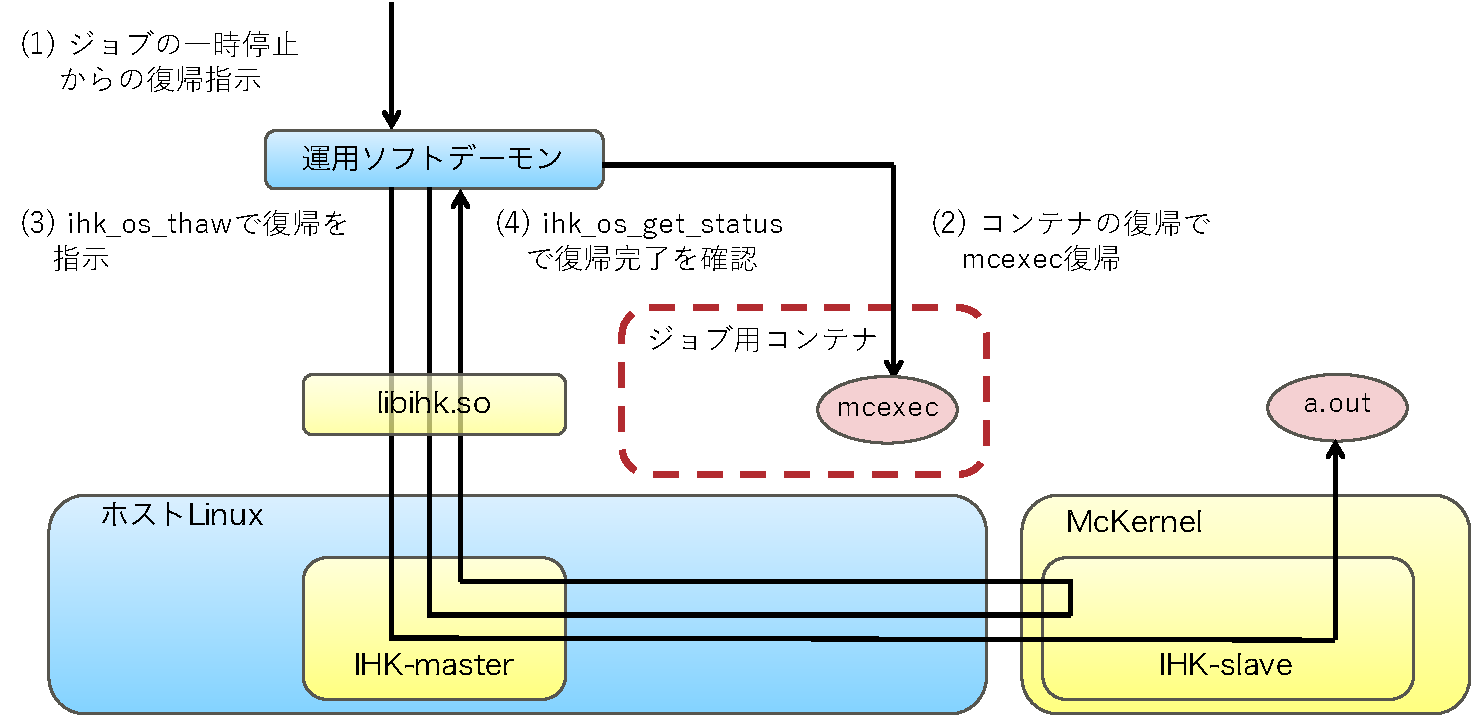
\includegraphics[width=14cm]{figs/thaw.pdf}
\vspace{-0em}\caption{全CPUの一時停止からの復帰のフロー}
\label{fig:thaw}
\vspace{-0em}
\end{figure}
%
全CPUの一時停止からの復帰の動作フローを図\ref{fig:thaw}を用いて説明する。
\begin{enumerate}
\item 運用ソフトがノードの運用ソフトデーモンにジョブの一時停止からの復帰を指示する。(図の(1))
\item 運用ソフトデーモンがコンテナの状態を変えることでmcexec (proxy process)を一時停止状態から復帰させる。(図の(2))
\item 運用ソフトデーモンが\texttt{ihk\_os\_thaw()}でMcKernelに全CPUの一時停止からの復帰を指示する。(図の(3))
\item 運用ソフトデーモンが\texttt{ihk\_os\_get\_status()}で全CPUの一時停止からの復帰完了を確認する。(図の(4))
\end{enumerate}
%
\FloatBarrier

\subsubsection*{戻り値}{\quad}
\begin{table}[!h]
\footnotesize
\begin{tabular}{|p{0.20\linewidth}|p{0.66\linewidth}|} \hline
0&正常終了\\ \hline
\ADDAUG{-EINVAL}&\begin{tabular}[t]{@{}l@{}}OSインスタンスのステータスが\\\texttt{IHK\_STATUS\_FREEZING}、\texttt{IHK\_STATUS\_FROZEN}以外\end{tabular}\\ \hline
\texttt{-EPERM}&操作に対する権限がない\\ \hline
\MODAUG{\texttt{-ENOENT}}&indexが示すOSインスタンスは存在しない\\ \hline
\end{tabular}
\vspace{-0em}
\end{table}
\FloatBarrier

\subsubsection{メモリダンプ採取}

\subsubsection*{書式}{\quad} \MODJULTWO{\texttt{int ihk\_os\_makedumpfile(int index, char *dump\_file, int dump\_level, int interactive)}}
\subsubsection*{説明}{\quad}
\texttt{index}で指定されたOSインスタンスについて、\MODJULTWO{\texttt{dump\_level}で指定されたメモリ領域を}\texttt{dump\_file}で指定したファイルに出力する。
\texttt{dump\_level}の指定方法は以下の通り。
\begin{table}[!h]
\footnotesize
\begin{tabular}{|p{0.10\linewidth}|p{0.76\linewidth}|} \hline
0&\MODJULTWO{IHKがOSインスタンスに割り当てたメモリ領域を出力する。}\\ \hline
24&\MODJULTWO{カーネルが使用しているメモリ領域を出力する。}\\ \hline
\end{tabular}
\vspace{-0em}
\end{table}
\FloatBarrier
\ADDJULTWO{\texttt{interactive}が1の場合は、interactive mode向けのファイルを出力する。このモードでは、ダンプ解析ツールはデバッグ対象マシンのメモリを直接参照して解析を行う。}
なお、この関数は特権ユーザのみ呼び出せる。

%McKernelの場合、NMIによってOSが停止するので、正規の手順で停止することができない。mcexecに\texttt{SIGKILL}を送って強制終了させること。

%McKernelの場合、ダンプの解析には、本コマンドが出力したダンプファイルの他に、カーネルイメージファイルが必要となる。必要なファイルの退避を忘れないこと。

\subsubsection*{戻り値}{\quad}
\begin{table}[!h]
\footnotesize
\begin{tabular}{|p{0.20\linewidth}|p{0.66\linewidth}|} \hline
0&正常終了\\ \hline
\texttt{-EPERM}&操作に対する権限がない\\ \hline
\texttt{-ENOENT}&\texttt{dump\_file}の値がNULL、または\texttt{dump\_file}が長さ0の文字列を指している、または\texttt{dump\_file}に含まれるディレクトリが存在しない\\ \hline
\texttt{-EACCES}&\texttt{dump\_file}で指定したファイルについて、ディレクトリは存在するがファイルが作成できない\\ \hline
\texttt{-EEXIST}&\texttt{dump\_file}で指定したファイルが既に存在する\\ \hline
\texttt{-EINVAL}&不正なパラメタ。\texttt{index}が負の場合を含む。\\ \hline
\texttt{-ENODEV}&\texttt{index}で指定されるOSインスタンスが存在しない\\ \hline
\texttt{-EPERM}&\texttt{index}で指定されるOSインスタンスにアクセスできない\\ \hline
\end{tabular}
\vspace{-0em}
\end{table}
\FloatBarrier

\subsection{LWK向けOS初期化機能}

\subsubsection{\MODAUGS{Get Number of NUMA Nodes}}
\subsubsection*{Synopsis}{\quad}
\declarefunc{int~ihk\_mc\_get\_nr\_numa\_nodes();}
\subsubsection*{Description}{\quad}
This function returns the number of NUMA nodes assigned by IHK.

\subsubsection*{Return Value}{\quad}
\begin{table}[!h]
\footnotesize
\begin{tabular}{|p{0.20\linewidth}|p{0.66\linewidth}|} \hline
$> 0$&The number of the NUMA nodes\\ \hline
\end{tabular}
\vspace{-0em}
\end{table}
\FloatBarrier

\subsubsection{\MODAUGS{Get NUMA Node Information}}
\subsubsection*{Synopsis}{\quad}
\declarefunc{int~ihk\_mc\_get\_numa\_node(int~id, int~*linux\_numa\_id, int~*type);}
\begin{funcdef}
\funcarg{id}{\IN}{NUMA id}
\funcarg{linux\_numa\_id}{\OUT}{Linux NUMA id}
\funcarg{type}{\OUT}{Memory type}
\end{funcdef}

\subsubsection*{Description}{\quad}
The host Linux NUMA id and the memory type of the NUMA node specified by \texttt{id} is stored to \texttt{linux\_numa\_id} and \texttt{type}, respectively. Each of the values is not stored when the corresponding pointer is NULL.

\subsubsection*{Return Value}{\quad}
\begin{table}[!h]
\footnotesize
\begin{tabular}{|p{0.20\linewidth}|p{0.66\linewidth}|} \hline
0&Success\\ \hline
-1&\texttt{id} is not valid\\ \hline
\end{tabular}
\vspace{-0em}
\end{table}
\FloatBarrier

\subsubsection{\ADDAUGS{Get NUMA id}}
\subsubsection*{Synopsis}{\quad}
\declarefunc{int~ihk\_mc\_get\_numa\_id();}

\subsubsection*{Description}{\quad}
Returns NUMA id of the CPU on which the caller is running on.

\subsubsection*{Return Value}{\quad}
\begin{table}[!h]
\footnotesize
\begin{tabular}{|p{0.20\linewidth}|p{0.66\linewidth}|} \hline
$\ge 0$&NUMA id\\ \hline
\end{tabular}
\vspace{-0em}
\end{table}
\FloatBarrier

\subsubsection{\ADDAUGS{Get Distance between NUMA Nodes}}
\subsubsection*{Synopsis}{\quad}
\declarefunc{int~ihk\_mc\_get\_numa\_distance(int i, int j);}

\subsubsection*{Description}{\quad}
Returns the distance between the NUMA nodes specified by \texttt{i} and \texttt{j}.
The distance matrix could be the same as Linux.

\subsubsection*{Return Value}{\quad}
\begin{table}[!h]
\footnotesize
\begin{tabular}{|p{0.20\linewidth}|p{0.66\linewidth}|} \hline
$\ge 0$&The distance between the NUMA nodes\\ \hline
\end{tabular}
\vspace{-0em}
\end{table}
\FloatBarrier

\subsubsection{\MODAUGS{Get Number of Memory Chunks}}
\subsubsection*{Synopsis}{\quad}
\declarefunc{int~ihk\_mc\_get\_nr\_memory\_chunks();}
\subsubsection*{Description}{\quad}
This function returns the number of physical memory chunks assigned by IHK.

\subsubsection*{Return Value}{\quad}
\begin{table}[!h]
\footnotesize
\begin{tabular}{|p{0.20\linewidth}|p{0.66\linewidth}|} \hline
$\ge 0$&The number of memory chunks\\ \hline
\end{tabular}
\vspace{-0em}
\end{table}
\FloatBarrier

\subsubsection{\MODAUGS{Get Memory Chunk Information}}
\subsubsection*{Synopsis}{\quad}
\declarefunc{int~ihk\_mc\_get\_memory\_chunk(int~id, unsigned long~*start, unsigned long~*end, int~*numa\_id);}

\subsubsection*{Description}{\quad}
The start physical address, end physical address and the NUMA id are stored to \texttt{start}, \texttt{end}, \texttt{numa\_id}, respectively. Each of the values is not stored when the corresponding pointer is NULL.

\subsubsection*{Return Value}{\quad}
\begin{table}[!h]
\footnotesize
\begin{tabular}{|p{0.20\linewidth}|p{0.66\linewidth}|} \hline
0&Success\\ \hline
-1&\texttt{id} is not valid\\ \hline
\end{tabular}
\vspace{-0em}
\end{table}
\FloatBarrier

\subsubsection{\MODAUGS{Get Number of Cores}}
\subsubsection*{Synopsis}{\quad}
\declarefunc{int~ihk\_mc\_get\_nr\_cores();}
\subsubsection*{Description}{\quad}
This function returns the number of CPU cores assigned by IHK.

\subsubsection*{Return Value}{\quad}
\begin{table}[!h]
\footnotesize
\begin{tabular}{|p{0.20\linewidth}|p{0.66\linewidth}|} \hline
$\ge 0$&The number of CPU cores\\ \hline
\end{tabular}
\vspace{-0em}
\end{table}
\FloatBarrier

\subsubsection{\MODAUGS{Get Core Information}}
\subsubsection*{Synopsis}{\quad}
\declarefunc{int~ihk\_mc\_get\_core(int~id, unsigned long~*linux\_core\_id, unsigned long~*hw\_id, int~*numa\_id);}

\subsubsection*{Description}{\quad}
The host Linux CPU id, the hardware id and the LWK NUMA id of the CPU core specified by \texttt{id} are stored to \texttt{linux\_core\_id}, \texttt{hw\_id}, \texttt{numa\_id}, respectively. Each of the values is not stored when the corresponding pointer is NULL. The hardware id corresponds to the hardware APIC id in \texttt{x86\_64} architecture.

\subsubsection*{Return Value}{\quad}
\begin{table}[!h]
\footnotesize
\begin{tabular}{|p{0.20\linewidth}|p{0.66\linewidth}|} \hline
0&Success\\ \hline
-1&\texttt{id} is not valid\\ \hline
\end{tabular}
\vspace{-0em}
\end{table}
\FloatBarrier

\subsubsection{\MODAUGS{Get IKC Destination CPU}}
\subsubsection*{Synopsis}{\quad}
\DIFFWG{\declarefunc{int~ihk\_mc\_get\_ikc\_cpu(int~id);}}

\subsubsection*{Description}{\quad}
This function returns the Linux id of the CPU to which the CPU specified by \texttt{id} sends IKC messages.
% see build_ihk_cpu_info() in setup.c
% see smp_ihk_os_boot() in smp-x86-driver.c

\subsubsection*{Return Value}{\quad}
\begin{table}[!h]
\footnotesize
\begin{tabular}{|p{0.20\linewidth}|p{0.66\linewidth}|} \hline
$\ge 0$&The Linux id of the IKC destination CPU\\ \hline
\end{tabular}
\vspace{-0em}
\end{table}
\FloatBarrier

\subsubsection{\MODAUGS{Get Kernel Arguments}}
\subsubsection*{Synopsis}{\quad}
\declarefunc{char~*ihk\_get\_kargs();}

\subsubsection*{Description}{\quad}
This function returns the pointer to the buffer containing the kernel arguments given by the IHK master.

\subsubsection*{Return Value}{\quad}
\begin{table}[!h]
\footnotesize
\begin{tabular}{|p{0.20\linewidth}|p{0.66\linewidth}|} \hline
$> 0$&The pointer to the kernel argument string\\ \hline
\end{tabular}
\vspace{-0em}
\end{table}
\FloatBarrier

%\input{ihk_ikc_set_master_queue}
% It's called by ihk_ikc_master_init

\subsubsection{\MODAUGS{Get Information of Kernel Message Buffer}}
\subsubsection*{Synopsis}{\quad}
\declarefunc{int~ihk\_get\_kmsg\_buf(unsigned long~*addr,
                 unsigned long~*size);}

\subsubsection*{Description}{\quad}
The physical address and the size of the kernel message buffer are stored to \texttt{addr} and \texttt{size}, respectively.
This function is supposed to be called when initializing LWK.

\subsubsection*{Return Value}{\quad}
\begin{table}[!h]
\footnotesize
\begin{tabular}{|p{0.20\linewidth}|p{0.66\linewidth}|} \hline
0&Success\\ \hline
\end{tabular}
\vspace{-0em}
\end{table}
\FloatBarrier

\comment{
\subsubsection{ihk\_remote\_physical\_to\_local\_physical}

\subsubsection*{Synopsis}{\quad}
\declarefunc{unsigned long~ihk\_remote\_physical\_to\_local\_physical(ihk\_os\_t~os, unsigned long~rphys);}
\begin{funcdef}
\funcarg{os}{\IN}{OS on the remote side. Zero means Linux. }
\funcarg{rphys}{\IN}{Physical address on the remote side}
\funcarg{size}{\IN}{Size of the memory area}
\end{funcdef}

\subsubsection*{Description}{\quad}
This function interpret the address specified by \texttt{rphys} as an address in the physical address space of the remote side and translate it into the address in the physical address space on the local side.
This function is available only to attached mode.
For example, Linux running on Xeon obtains a physical address of LWK running on Xeon Phi and translates it into the physical address of Xeon using this function. 

\texttt{ihk\_os\_t} is an opaque type representing an OS.

% It points to (\texttt{struct ihk\_host\_linux\_os\_data)} and it must have at least the following member. Using \texttt{void*} for \texttt{priv} makes it possible to switch the architeture dependent structures (e.g. \texttt{struct mic\_os\_data}).
%
% It's defined as follows.
% \begin{verbatim}
% typedef void *ihk_os_t;
% struct ihk_host_linux_os_data {
%  ...
%    void *priv;
%  ...
% };
% \end{verbatim}
% 
% \begin{description}
% \item[{\tt priv}]{Storing a pointer to architecture dependent structure, e.g. \texttt{struct mic\_os\_data}}
% \end{description}

\subsubsection*{Return Value}{\quad}
Address in physical address space on the local (caller) side
}

\subsubsection{\MODAUGS{Boot a Core}}
\subsubsection*{Synopsis}{\quad}
\declarefunc{void ihk\_mc\_boot\_cpu(int cpu\_id, unsigned long pc);}
\subsubsection*{Description}{\quad}
This function makes the CPU specified by \texttt{cpu\_id} (Physical APIC CPU ID) start execution from the virtual address specified by \texttt{pc}.

\subsection{LWK向けInter-Kernel Communication (IKC)機能}\label{sec:ikc}

\subsubsection{\MODAUGS{Initialize Master Channel on the IHK-master side}}
\subsubsection*{Synopsis}{\quad}
\declarefunc{int ihk\_ikc\_master\_init(ihk\_os\_t os);}

\subsubsection*{Description}{\quad}
This function is called by Linux and initializes the master channel connected to the OS specified by \texttt{os}.
The master channel is present at boot time and used for creating / destroying more channels.
The created channel is called regular channel and used for the communication.
LWK sends a connection request to Linux through the master channel to create a regular channel.

\subsubsection*{Return Value}{\quad}
\begin{table}[!h]
\footnotesize
\begin{tabular}{|p{0.20\linewidth}|p{0.66\linewidth}|} \hline
0&Success\\ \hline
$\ne 0$&Error number\\ \hline
\end{tabular}
\vspace{-0em}
\end{table}
\FloatBarrier

\subsubsection{\MODAUGS{Initialize Master Channel on the IHK-slave side}}
\subsubsection*{Synopsis}{\quad}
\declarefunc{void ihk\_ikc\_master\_init(void);}
\subsubsection*{Description}{\quad}
This function is called by LWK and initializes the master channel connected to Linux.

% \begin{figure}[h]
% \centering
% \includegraphics[width=12cm]{figs/master_channel.pdf}
% \vspace{-0em}\caption{Structure of the IKC master channel.}
% \label{fig:master_channel}
% \vspace{-0em}
% \end{figure}
% The master channel is represented by \texttt{struct ihk\_ikc\_channel\_desc} and its structure is explained using Fig. \ref{fig:master_channel}.
% Both of queues are located in memory local to the IHK-slave.
% The IHK slave writes packets onto the memory local to it and the IHK master reads the packets from there.
% The IHK master writes packets onto the memory remote to it and the IHK slave reads the packets from there.
% \texttt{read\_cpu} records the CPU ID of the reader and \texttt{write\_cpu} records that of the writer for Inter-Processor Interrupt.
% Its declaration is shown in \ref{sec:regular_channel} for more information.

\subsubsection{\MODAUGS{Listen to Connection Requests}}
\subsubsection*{Synopsis}{\quad}
\declarefunc{int ihk\_ikc\_listen\_port(ihk\_os\_t os, struct ihk\_ikc\_listen\_param *param);}
\subsubsection*{Description}{\quad}
This function makes the master channel listen to the remote OS specified by \texttt{os} to create a channel with the parameters of \texttt{param}. 
% \begin{figure}[h]
% \centering
% \includegraphics[width=12cm]{figs/connection.pdf}
% \vspace{-0em}\caption{Timeline diagram of connection.}
% \label{fig:connection}
% \vspace{-0em}
% \end{figure}
% Fig. \ref{fig:connection} shows the timeline diagram of the protocol.
% The protocol proceeds as follows.
% \begin{enumerate}
% \item The IHK-slave (blue) prepares a partial channel, i.e. receive queue
% \item The IHK-slave connects to the IHK-master via port $N$
% \item The IHK-master (red) creates a new channel
% \item The IHK-master replies back the queue information to the IHK-slave X
% \item The IHK-slave sets IHK-master's local queue as channel's remote queue
% \end{enumerate}

\texttt{struct ihk\_ikc\_listen\_param} specifies parameters for a channel to be created and defined as follows.
\begin{verbatim}
struct ihk_ikc_listen_param {
    int (*handler)(struct ihk_ikc_channel_info *);
    int port;
    int pkt_size;
    int queue_size;
    int magic;
    int recv_cpu;
};
\end{verbatim}
\begin{structdef}
\typefield{\tt handler}{A function called when accepting an incoming connection request}
\typefield{\tt port}{Port number}
\typefield{\tt pkt\_size}{Packet size}
\typefield{\tt queue\_size}{Queue size}
\typefield{\tt magic}{Magic number for identification of the communication initiator}
\typefield{\tt recv\_cpu}{CPU ID of the listener}
\end{structdef}
%A function whose pointer is set to \texttt{handler} is assumed to perform the followings and must be prepare the LWK.
%\item Sets the call-back function which is called when detecting an arrival of a packet.
An IHK user must set the first four fields before passing it to \texttt{ihk\_ikc\_listen\_port}.
The IHK user must define function which is set to \texttt{handler} field of this structure.
%The function is registered when calling \texttt{ihk\_ikc\_listen\_port.}
\texttt{handler} is called when accepting an incoming connection request and it is expected to set \texttt{packet\_handler} field of the argument.
The value of the field is then copied to \texttt{handler} field of \texttt{ihk\_ikc\_channel\_desc} and becomes the call-back function which is called when detecting an arrival of a packet.
This accept-time call-back mechanism is used to create a table which is indexed by a CPU ID and returns the channel bound to the CPU.
%\end{quote}

\texttt{ihk\_ikc\_channel\_info} is an intermediate object used by the accept-time call-back function to pass the packet-arrival-time call-back function to the channel as described above and is defined as follows.
\begin{verbatim}
struct ihk_ikc_channel_info {
    struct ihk_ikc_channel_desc *channel;
    ihk_ikc_ph_t packet_handler;
};
\end{verbatim}
\texttt{channel} is only used internally.
\texttt{packet\_handler} is a pointer to the packet-arrival-time call-back function and is set by the accept-time call-back function.

\subsubsection*{Return Value}{\quad}
\begin{table}[!h]
\footnotesize
\begin{tabular}{|p{0.20\linewidth}|p{0.66\linewidth}|} \hline
0&Success\\ \hline
$\ne 0$&Error number\\ \hline
\end{tabular}
\vspace{-0em}
\end{table}
\FloatBarrier

% called by mckernel/executer/kernel/ikc.c
% not internal to the IHK library
\subsubsection{\MODAUGS{Send a Connection Request}}
\subsubsection*{Synopsis}{\quad}
\declarefunc{int ihk\_ikc\_connect(ihk\_os\_t os, struct ihk\_ikc\_connect\_param *p);}
\subsubsection*{Description}{\quad}
This function sends a connection request to the remote OS specified by \texttt{os} via the master channel to create a regular channel with the parameters of \texttt{p}. The created channel is stored to \texttt{p->channel}.
The receiver side detects the arrival of a packet either by calling non-blocking receive function or by notification (IRQ) and call-back mechanism.
%IHK-slave calls this function to connect to IHK-master.

% \begin{figure}[h]
% \centering
% \includegraphics[width=12cm]{figs/regular_channel.pdf}
% \vspace{-0em}\caption{Structure of an IKC regular channel.}
% \label{fig:regular_channel}
% \vspace{-0em}
% \end{figure}
% \texttt{ihk\_ikc\_channel\_desc} also represents the regular channel and its structure is explained using Fig. \ref{fig:regular_channel}.
% The receive queue is located in local memory and the send queue is locate in remote memory.
% Remote memory means the physical memory of the peer kernel.
% The IHK slave writes packets onto the memory local to it and the IHK master reads the packets from there.
% The IHK master writes packets onto the memory remote to it and the IHK slave reads the packets from there.

\texttt{ihk\_ikc\_connect\_param} specifies the parameters for the channel to be created and is defined as follows.
\begin{verbatim}
struct ihk_ikc_connect_param {
    int port;
    int pkt_size;
    int queue_size;
    int magic;
    ihk_ikc_ph_t               handler;
    struct ihk_ikc_channel_desc *channel;
};
\end{verbatim}
\begin{structdef}
\typefield{\tt port}{Port number}
\typefield{\tt pkt\_size}{Packet size}
\typefield{\tt queue\_size}{Queue size}
\typefield{\tt magic}{Magic number for identification of the communication initiator}
\typefield{\tt handler}{Packet handler called when calling \texttt{ihk\_ikc\_recv\_handler}}
\typefield{\tt channel}{Channel descriptor which is set when connected}
\end{structdef}
An IHK user must set \texttt{port, pkt\_size, queue\_size, magic, handler} fields.
\texttt{channel} field is set to the descriptor of the channel.

\texttt{ihk\_ikc\_channel\_desc} is an opaque type represeinting an IKC channel.
% \begin{verbatim}
% struct ihk_ikc_channel_desc {
%     struct list_head           list;
%     ihk_os_t                   remote_os;
%     int                        remote_channel_id;
%     int                        port;
%     int                        channel_id;
%     struct ihk_ikc_queue_desc  recv, send;
%     ihk_spinlock_t             lock;
%     enum ihk_ikc_channel_flag  flag;
%     ihk_ikc_ph_t               handler;
%     char                       packet_buf[0];
% };
% \end{verbatim}
% %\begin{verbatim}
% %    struct list_head           all_list;
% %\end{verbatim}
% %is eliminated because it's not used.
% \begin{description}
% \item[{\tt list}]{List of channels}
% \item[{\tt remote\_os}]{OS on the responder side}
% \item[{\tt remote\_channel\_id}]{Unique number for the channel on the responder side}
% \item[{\tt port}]{Port number}
% \item[{\tt channel\_id}]{Unique number for the channel on the initiator side}
% \item[{\tt recv}]{Receive queue}
% \item[{\tt send}]{Send queue}
% \item[{\tt lock}]{Lock variable}
% \item[{\tt flag}]{Channel flags}
% \item[{\tt handler}]{A function which is called when an incoming packet arrives.}
% \item[{\tt packet\_buf}]{Used to point at the start address of the ring-buffer. }
% \item[{\tt template}]{Template}
% \end{description}

%\input{ihk_ikc_queue_desc}
%(internal to the IHK library)
%\input{ihk_ikc_queue_head}
%(internal to the IHK library)
%\input{ihk_ikc_channel_flag}
%(internal to the IHK library)

% \begin{figure}[h]
% \centering
% \includegraphics[width=12cm]{figs/queue_structure.pdf}
% \vspace{-0em}\caption{Structure of an IKC queue.}
% \label{fig:queue_structure}
% \vspace{-0em}
% \end{figure}
% \texttt{struct ihk\_ikc\_queue\_head} represents IKC queue.
% Fig. \ref{fig:queue_structure} shows its structure.
% It consists of a header and ring-buffer.
% One packet has a fixed size of \texttt{pkt\_size} bytes.
% The ring-buffer has a fixed size, that is, \texttt{pkt\_count} of \texttt{pkt\_size}-sized slots.
% \texttt{read\_off} denotes the consumer pointer of the ring-buffer and
% \texttt{write\_off} denotes the producer pointer fo the ring-buffer.
%The \texttt{qhead} header has the following fields.
%\begin{description}
%\item[{\tt channel\_id}]{ID of the related channel}
%\item[{\tt pkt\_size}]{Size of a packet in byte}
%\item[{\tt pkt\_count}]{Max number of packets in a queue}
%\item[{\tt read\_off}]{Read offset in byte}
%\item[{\tt write\_off}]{Write offset in byte}
%\item[{\tt read\_cpu}]{Reader’s cpu ID}
%\end{description}

\subsubsection*{Return Value}{\quad}
\begin{table}[!h]
\footnotesize
\begin{tabular}{|p{0.20\linewidth}|p{0.66\linewidth}|} \hline
0&Success\\ \hline
$\ne 0$&Error number\\ \hline
\end{tabular}
\vspace{-0em}
\end{table}
\FloatBarrier

% \input{ihk_ikc_accept}
% (internal to the IHK library)

%\input{ihk_ikc_recv}
% (internal to the IHK library)
\subsubsection{\MODAUGS{Register a Call-Back Function for Receive Events}}
\subsubsection*{Synopsis}{\quad}
\declarefunc{int ihk\_ikc\_recv\_handler(struct ihk\_ikc\_channel\_desc *channel,
                         ihk\_ikc\_ph\_t h, void *harg, int opt);
}
\subsubsection*{Description}{\quad}
This function registers to the channel specified by \texttt{channel} a call-back function specified by \texttt{h} and an argument passed to it specified by \texttt{harg}. The call-back function is called when a packet arrives.
The call-back function handles multiple packets that have arrived and performs only one notification action (e.g. sends an interrupt to the sender side).
\texttt{NO\_COPY} bit of \texttt{opt} should be set to zero when the packet is accessed by the code outside the handler.

{\tt ihk\_ikc\_ph\_t} represents the call-back function which is called when detecting an arrival of an incoming packet and is defined as follows.
\begin{verbatim}
typedef int (*ihk_ikc_ph_t)(struct ihk_ikc_channel_desc *, void *, void *);
\end{verbatim}
It takes the descriptor of IKC channel as the first argument, the address of the incoming packet as the second argument and \texttt{harg} passed by \texttt{ihk\_ikc\_recv\_handler} as the third argument.

\texttt{harg} supports the use case where an IHK user can bind an abstracted channel structure used in the IHK user module to the IKC channel so that the handler can identify the abstracted channel through which the packet has arrived.
A reverse search table which returns the abstracted channel given the IKC channel ID is needed if \texttt{harg} is not passed down to the call-back function.

\subsubsection*{Return Value}{\quad}
\begin{table}[!h]
\footnotesize
\begin{tabular}{|p{0.20\linewidth}|p{0.66\linewidth}|} \hline
0&Success\\ \hline
$\ne 0$&Error number\\ \hline
\end{tabular}
\vspace{-0em}
\end{table}
\FloatBarrier

\subsubsection{\MODAUGS{Send a Packet}}
\subsubsection*{Synopsis}{\quad}
\declarefunc{int ihk\_ikc\_send(struct ihk\_ikc\_channel\_desc *channel, void *p, int opt);}
\subsubsection*{Description}{\quad}
This function sends a packet specified by \texttt{p} through a regular channel specified by \texttt{channel}.
It performs a notification action to the receiver side (e.g. sends an interrupt) when \texttt{IKC\_NO\_NOTIFY} bit of \texttt{opt} is zero.
It is safe to overwrite memory area pointed by \texttt{p} after calling \texttt{ihk\_ikc\_send} because the packet is memory-copied before sending.
It is the IHK user's responsibility to perform flow control.
\subsubsection*{Return Value}{\quad}
\begin{table}[!h]
\footnotesize
\begin{tabular}{|p{0.20\linewidth}|p{0.66\linewidth}|} \hline
0&Success\\ \hline
$\ne 0$&Error number\\ \hline
\end{tabular}
\vspace{-0em}
\end{table}
\FloatBarrier

% \begin{figure}[h]
% \centering
% \includegraphics[width=12cm]{figs/disconnect.pdf}
% \vspace{-0em}\caption{Timeline diagram of disconnection.}
% \label{fig:disconnect}
% \vspace{-0em}
% \end{figure}
% Fig. \ref{fig:disconnect} shows the timeline diagram of the protocol.
% The protocol proceeds as follows.
% \begin{enumerate}
% \item The Kernel X (blue) marks the recv as “destroying”
% \item Kernel X sends a disconnect message to Kernel Y
% \item Kernel Y marks its recv queue as “destroying” and destroys the channel
% \item Kernel Y sends a disconnect message to Kernel X
% \item Kernel X destroys the channel
% \item \end{enumerate}

\subsubsection{\MODAUGS{Disconnect a Channel}}
\subsubsection*{Synopsis}{\quad}
\declarefunc{int ihk\_ikc\_disconnect(struct ihk\_ikc\_channel\_desc~*c);}
\subsubsection*{Description}{\quad}
This function disconnects a regular channel specified by \texttt{c}.

\subsubsection*{Return Value}{\quad}
\begin{table}[!h]
\footnotesize
\begin{tabular}{|p{0.20\linewidth}|p{0.66\linewidth}|} \hline
0&Success\\ \hline
$\ne 0$&Error number\\ \hline
\end{tabular}
\vspace{-0em}
\end{table}
\FloatBarrier

% \input{ihk_ikc_free_channel}
% Linux kernel part of IHK library needs to remove va-pa mapping and return physical pages to OS,
% but it's internal processing.
% LWK part of IHK library don't need to perform a special thing.

\subsubsection{\MODAUGS{Destroy a Channel}}
\subsubsection*{Synopsis}{\quad}
\declarefunc{void ihk\_ikc\_destroy\_channel(struct ihk\_ikc\_channel\_desc *c);}
\subsubsection*{Description}{\quad}
This function destroys the master channel or a regular channel specified by \texttt{c}.

\subsection{Linuxドライバ向け機能}
\subsubsection{制御レジスタリード}
% \subsubsection*{名前}{\quad} \texttt{ihk\_os\_read\_cpu\_register}
\subsubsection*{書式}{\quad} \texttt{int ihk\_os\_read\_cpu\_register(ihk\_os\_t os, int cpu, struct ihk\_os\_cpu\_register *desc)}
\subsubsection*{説明}{\quad}
\texttt{os}で指定するOSインスタンスの\texttt{cpu}で指定するCPUの\texttt{desc}で指定する制御レジスタ値を\texttt{desc->val}へ非同期で読み込む。完了は\texttt{desc->sync}のゼロ以外の値への変化で検知できる。なお、\texttt{cpu}にはLWKでの番号を指定する。また、呼び出し元が\texttt{desc}の領域を用意する。

\texttt{struct ihk\_os\_cpu\_register}は以下のように定義される。
\begin{Verbatim}[commandchars=\\\{\}]
struct ihk_os_cpu_register \{
    unsigned long addr;
\textcolor{red}{    /* メモリマップの制御レジスタのアドレス。アーキテクチャ固有の値}
\textcolor{red}{       をそのまま用いる。*/}
    unsigned long addr_ext;
\textcolor{red}{    /* CPUの制御レジスタ番号。アーキテクチャ固有の値をそのまま用いる。*/}
\textcolor{red}{    unsigned long val;}
    /* ihk_os_write_cpu_register():制御レジスタに書き込む値
       ihk_os_read_cpu_register():制御レジスタ値の記録先 */
    atomic_t sync;
    /* 制御レジスタへの操作完了を示す。0は未完了を意味し、0以外は完了を
       意味する。*/
\};
\end{Verbatim}

利用のステップを図\ref{fig:cpu_register}を用いて説明する。
\begin{enumerate}
\item LWK上で動作するライブラリがLWKからのオフロード経由でLinuxドライバにレジスタ操作を指示する場合は、\texttt{ihk\_get\_request\_os\_cpu()}を用いてオフロード元OSインスタンスとCPU番号を取得する。こうすることで、操作先のOSインスタンス偽装を防ぐ。(図の(1))
\item Linuxドライバが操作完了を示す変数を未完了(0)に設定してから、\texttt{ihk\_os\_read\_cpu\_register()}または\texttt{ihk\_os\_write\_cpu\_register()}でレジスタを非同期に操作する。(図の(2))
\item IHKまたはLWKが上記変数の値を変化させることにより操作完了をLinuxドライバに通知する。(図の(3))
\end{enumerate}
%
\begin{figure}[!htb]
\centering
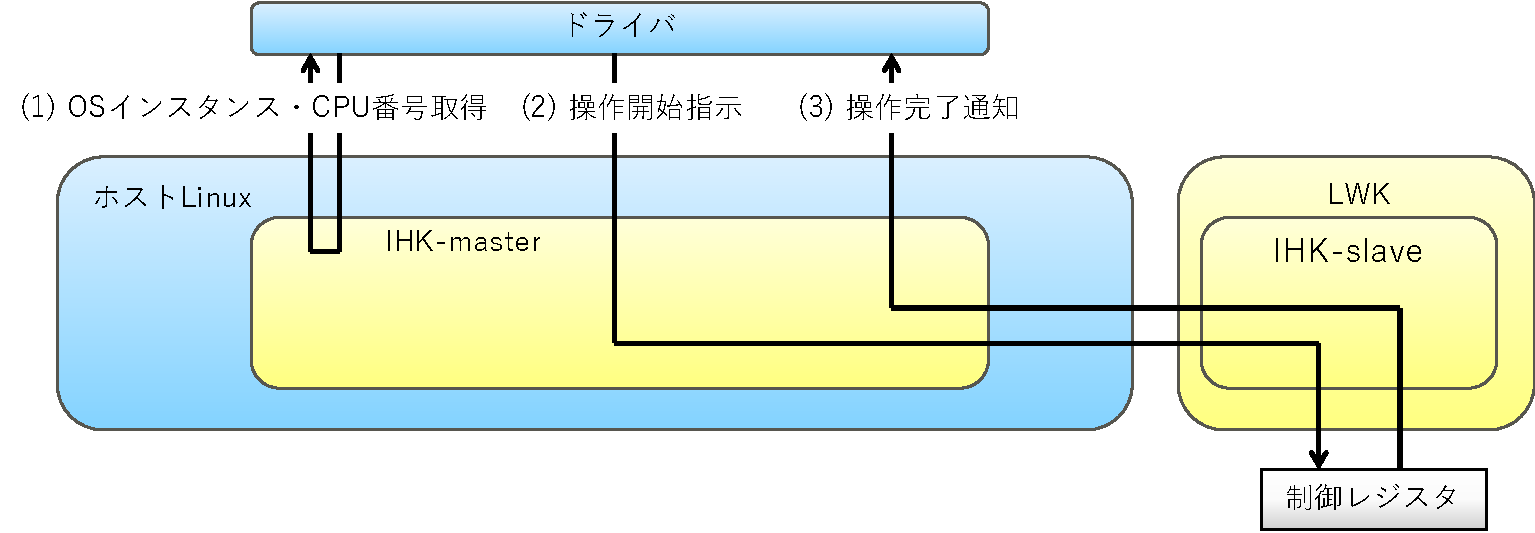
\includegraphics[width=14cm]{figs/cpu_register.pdf}
\vspace{-0em}\caption{制御レジスタの操作ステップ}
\label{fig:cpu_register}
\vspace{-0em}
\end{figure}
\FloatBarrier

\subsubsection*{戻り値}
\begin{table}[!h]
\footnotesize
\begin{tabular}{|p{0.20\linewidth}|p{0.66\linewidth}|} \hline
0&正常終了\\ \hline
\texttt{-EINVAL}&\texttt{os}にアクセスできない、または\texttt{cpu}がLWKに割り当てられているCPUではない、または指定されたアドレスまたは番号のレジスタは存在しない\\ \hline
\texttt{-EFAULT}&\texttt{desc}にアクセスできない\\ \hline
\verb:-ENOMEM:&メモリ不足が発生した\\ \hline
\verb:-ETIME:&LWKが応答しなかった\\ \hline
\verb:-ERESTARTSYS:&LWKの応答を待っている間にシグナルにより割り込まれた\\ \hline
\end{tabular}
\vspace{-0em}
\end{table}
\FloatBarrier

\subsubsection{制御レジスタライト}
\subsubsection*{書式}{\quad} \texttt{int ihk\_os\_write\_cpu\_register(ihk\_os\_t os, int cpu, struct ihk\_os\_cpu\_register *desc)}
\subsubsection*{説明}{\quad}
\texttt{os}で指定するOSインスタンスの\texttt{cpu}で指定するCPUの\texttt{desc}で指定する制御レジスタへ\texttt{desc->val}で指定する値を非同期で書き込む。完了は\texttt{desc->sync}のゼロ以外の値への変化で検知できる。 なお、\texttt{cpu}にはLWKでの番号を指定する。

\subsubsection*{戻り値}
\begin{table}[!h]
\footnotesize
\begin{tabular}{|p{0.20\linewidth}|p{0.66\linewidth}|} \hline
0&正常終了\\ \hline
\texttt{-EINVAL}&\texttt{os}にアクセスできない、または\texttt{cpu}がLWKに割り当てられているCPUではない、または指定されたアドレスまたは番号のレジスタは存在しない\\ \hline
\texttt{-EFAULT}&\texttt{desc}にアクセスできない\\ \hline
\verb:-ENOMEM:&メモリ不足が発生した\\ \hline
\verb:-ETIME:&LWKが応答しなかった\\ \hline
\verb:-ERESTARTSYS:&LWKの応答を待っている間にシグナルにより割り込まれた\\ \hline
\end{tabular}
\vspace{-0em}
\end{table}
\FloatBarrier

\subsubsection{オフロード元OSインスタンス取得}
\subsubsection*{書式}{\quad} \DIFFWG{\texttt{int ihk\_get\_request\_os\_cpu(ihk\_os\_t *os, int *cpu)}}
\subsubsection*{説明}{\quad}
システムコール移譲などのオフロード経由で本関数の呼び出しを行った場合、オフロード元LWKのOSインスタンスを\texttt{os}に、CPU番号を\texttt{cpu}に返す。なお、\texttt{cpu}はMcKernelでの番号である。

\subsubsection*{戻り値}
\begin{table}[!h]
\footnotesize
\begin{tabular}{|p{0.20\linewidth}|p{0.66\linewidth}|} \hline
0&正常終了\\ \hline
\texttt{-EINVAL}&オフロードにより当該呼び出しにいたっていない\\ \hline
\texttt{-EFAULT}&\texttt{os}または\texttt{cpu}にアクセスできない\\ \hline
\end{tabular}
\vspace{-0em}
\end{table}
\FloatBarrier

\section{\MODAUGS{コマンド・デーモン仕様}}\label{sec:ihk_commands}

\subsection{管理者向け資源管理機能}
\comment{
\subsubsection{Usage Example}
This section shows a quick usage example of IHK's resource partitioning
functionality and demonstrates the interaction with LWK instances
in case of using the IHK-SMP x86 driver module.

The manycore device representing resources
on an SMP node can be then manipulated via ioctl() calls to the
device file \texttt{/dev/mcd0}, for which the \texttt{ihkconfig} command line
tool is provided.
The modules do not reserve any resources at load time (except for a couple
of small datastructures).

IHK-SMP x86 uses the Linux kernel's hotplug system to detach CPU cores from Linux.
In order to reserve CPU cores for the IHK framework, one needs to issue the
following command:

\begin{verbatim}
$ ihkconfig 0 reserve cpu 2-4,10
\end{verbatim}

The example above reserves CPUs with logical IDs 2,3,4 and 10.
For detailed explanation on the CPU ID format see Section \ref{sec:reserve_cpu}.
Note that CPU 0 is not permitted to be reserved for IHK and it always remains
for use by Linux.

Similarly, memory can be reserved for the IHK framework using the following
command:

\begin{verbatim}
$ ihkconfig 0 reserve mem 2048M
\end{verbatim}

The number specified indicates the number of bytes, but it can be simplified with the
addition of standard metric prefixes (i.e., \texttt{k}, \texttt{M}, \texttt{G} etc.).
The above example reserves 2GBs of physical memory.
For simplicity, we have not
specified NUMA related information here, see Section \ref{sec:reserve_mem} for NUMA
specific memory allocation.
In summary, at this point IHK holds 4 CPU cores and 2 GBs of memory.

In order to actually load and boot a kernel image first an OS
instance needs to be created by executing the following command:

\begin{verbatim}
$ ihkconfig 0 create
\end{verbatim}

After this command executed, a new device file (e.g., \texttt{/dev/mcos0}) is
created that represents the new OS.
}

\subsubsection{\MODJULTWOS{Reserve CPUs}}\label{sec:reserve_cpu}
\subsubsection*{Synopsis}{\quad} \texttt{ihkconfig <dev index> reserve cpu <CPU id list>}
\subsubsection*{Description}{\quad}
This command reserves specific CPU cores for the IHK framework.
\texttt{<dev index>} identifies
the IHK device file that appears as the result of the insertion of the
IHK-master driver module, and \texttt{<CPU id list>} is the following format:
\texttt{<CPU logical id>},...,\texttt{<CPU logical id>} or
\texttt{<CPU logical id>} - \texttt{<CPU logical id>}
(must be a positive range in ascending order)
or a mixture of the two: \texttt{<CPU logical id>},...,\texttt{<CPU logical
id>} - \texttt{<CPU logical id>}.
CPU logical ID begins at 0 and the maximum value is "number of CPUs in system - 1".
An actual example of usage would be:

\begin{verbatim}
$ ihkconfig 0 reserve cpu 24-31
\end{verbatim}

The reserve operation may be executed multiple times adding
CPU logical ID cores as required.

\subsubsection*{\ADDJULTWOS{Exit Status}}
\begin{table}[!h]
\footnotesize
\begin{tabular}{|p{0.20\linewidth}|p{0.66\linewidth}|} \hline
0&Success\\ \hline
Other than 0&Failure\\ \hline
\end{tabular}
\vspace{-0em}
\end{table}
\FloatBarrier

\subsubsection{\MODJULTWOS{Query CPUs}}
\subsubsection*{Synopsis}{\quad} \texttt{ihkconfig <dev index> query cpu}
\subsubsection*{Description}{\quad}
This command queries which CPU cores the IHK framework has reserved.
\texttt{<dev index>} identifies
the IHK device file that appears as the result of the insertion of the
IHK-master driver module.

The command returns the list of CPUs in the same format as the above
reservation command.

\subsubsection*{\ADDJULTWOS{Exit Status}}
\begin{table}[!h]
\footnotesize
\begin{tabular}{|p{0.20\linewidth}|p{0.66\linewidth}|} \hline
0&Success\\ \hline
Other than 0&Failure\\ \hline
\end{tabular}
\vspace{-0em}
\end{table}
\FloatBarrier

\subsubsection{\MODJULTWOS{Release CPUs}}
\subsubsection*{Synopsis}{\quad} \texttt{ihkconfig <dev index> release cpu <CPU id list>}
\subsubsection*{Description}{\quad}
This command releases the specific CPU cores from the IHK framework.
\texttt{<dev index>} identifies
the IHK device file that appears as the result of the insertion of the
IHK-master driver module,
and \texttt{<CPU id list>} is the following format:
\texttt{<CPU logical id>},...,\texttt{<CPU logical id>} or
\texttt{<CPU logical id>} - \texttt{<CPU logical id>}
(must be a positive range in ascending order)
or a mixture of the two: \texttt{<CPU logical id>},...,\texttt{<CPU logical
id>} - \texttt{<CPU logical id>}.
CPU logical ID begins at 0 and the maximum value is "number of CPUs in system - 1".
An actual example of usage would be:

\begin{verbatim}
$ ihkconfig 0 release cpu 24-31
\end{verbatim}

The release operation may be executed multiple times removing
CPU logical ID cores from IHK as required.

\subsubsection*{\ADDJULTWOS{Exit Status}}
\begin{table}[!h]
\footnotesize
\begin{tabular}{|p{0.20\linewidth}|p{0.66\linewidth}|} \hline
0&Success\\ \hline
Other than 0&Failure\\ \hline
\end{tabular}
\vspace{-0em}
\end{table}
\FloatBarrier

\subsubsection{\MODPREVS{Reserve Memory}}\label{sec:reserve_mem}
\subsubsection*{Synopsis}{\quad} \texttt{ihkconfig <dev index> reserve mem <memory description>}
\subsubsection*{Description}{\quad}
This command reserves memory for the IHK framework.
\texttt{<dev index>} identifies
the IHK device file that appears as the result of the insertion of the
IHK-master driver module.
You can specify the size and the NUMA nodes with the \verb|<memory description>| argument by using the following format:
\begin{verbatim}
(<size>[<unit>]|ALL)[@<NUMA-id>][,(<size>[<unit>]|ALL)[@<NUMA-id>]...]
\end{verbatim}
where \texttt{<size>} is the number of bytes requested, optionally followed by a unit (\texttt{M}, \texttt{G} and \texttt{T} are available, meaning MiB, GiB and TiB, respectively).
Moreover, the optional \texttt{@} symbol that can be followed by a decimal number
denotes the targeted NUMA node, where the default NUMA node is 0.
Specifying \verb:ALL: in the size field means request for best effort maximum.

Here is an example which allocates 2 Gigabytes from NUMA node 1:
\begin{verbatim}
$ ihkconfig 0 reserve mem 2G@1
\end{verbatim}

The reserve operation may be executed multiple times adding
physical memory as required. The operation may fail in case the system wide
available memory is less than the amount requested.
IHK reserves the memory area of the requested size using the following alorithm.
We denote by $s$ the requested size and by $t$ the total size of the reserved memory-chunks.
\begin{enumerate}
\item Find the largest memory chunk with the size of less than or equal to $s-t$ and reserve it.
\item Repeat the above step until $t$ becomes equals to $s$.
\end{enumerate}

\subsubsection*{\ADDJULTWOS{Exit Status}}
\begin{table}[!h]
\footnotesize
\begin{tabular}{|p{0.20\linewidth}|p{0.66\linewidth}|} \hline
0&Success\\ \hline
Other than 0&Failure\\ \hline
\end{tabular}
\vspace{-0em}
\end{table}
\FloatBarrier

\subsubsection{\MODJULTWOS{Query Memory}}
\subsubsection*{Synopsis}{\quad} \texttt{ihkconfig <dev index> query mem}
\subsubsection*{Description}{\quad}
This command queries the amount of the memory that the IHK framework has reserved and has not been assigned to an OS instance.
\texttt{<dev index>} identifies
the IHK device file that appears as the result of the insertion of the
IHK-master driver module.

The command returns the list of memory regions in the same format as the above
reservation command.

\subsubsection*{\ADDJULTWOS{Exit Status}}
\begin{table}[!h]
\footnotesize
\begin{tabular}{|p{0.20\linewidth}|p{0.66\linewidth}|} \hline
0&Success\\ \hline
Other than 0&Failure\\ \hline
\end{tabular}
\vspace{-0em}
\end{table}
\FloatBarrier

\subsubsection{Release Memory}
\subsubsection*{Synopsis}{\quad}\texttt{ihkconfig <dev index> release mem <memory list>}
\subsubsection*{Description}{\quad}
This command releases memory from the IHK framework.
\texttt{<dev index>} identifies
the IHK device file that appears as the result of the insertion of the
IHK-master driver module.
The \texttt{<memory list>} takes the same format as the above reserve command. \texttt{all} means to release all of the reserved memory.
An actual example of usage would be:

\begin{verbatim}
$ ihkconfig 0 release mem 1G@1
\end{verbatim}

The release operation may be executed multiple times freeing
physical memory as required.
The operation may fail in case the IHK reserved
memory is less than the amount requested.

\subsubsection*{\ADDJULTWOS{Exit Status}}
\begin{table}[!h]
\footnotesize
\begin{tabular}{|p{0.20\linewidth}|p{0.66\linewidth}|} \hline
0&Success\\ \hline
Other than 0&Failure\\ \hline
\end{tabular}
\vspace{-0em}
\end{table}
\FloatBarrier

\subsubsection{\MODJULTWOS{Create OS instance}}
\subsubsection*{Synopsis}{\quad} \texttt{ihkconfig <dev index> create}
\subsubsection*{Description}{\quad}
This command creates an OS instance over the specific IHK device.
\texttt{<dev index>} identifies the IHK device file that appears as the result of the insertion of the IHK-master driver module.
An actual example of usage would be:

\begin{verbatim}
$ ihkconfig 0 create
\end{verbatim}

Unless an error occurs, the command returns an index \texttt{X} which will denote the
specific OS device file with path name of \texttt{/dev/mcosX}.

\subsubsection*{\ADDJULTWOS{Exit Status}}
\begin{table}[!h]
\footnotesize
\begin{tabular}{|p{0.20\linewidth}|p{0.66\linewidth}|} \hline
0&Success\\ \hline
Other than 0&Failure\\ \hline
\end{tabular}
\vspace{-0em}
\end{table}
\FloatBarrier

\subsubsection{\MODJULTWOS{Destroy OS instance}}
\subsubsection*{Synopsis}{\quad} \texttt{ihkconfig <dev index> destroy <os index>}
\subsubsection*{Description}{\quad}
\MODJULTWO{This command destroys the OS instance specified by \texttt{<os index>} residing on the IHK device specified by \texttt{<dev index>}. The resources assigned to the OS instance are released before destroying it.}
An actual example of usage would be:

\begin{verbatim}
$ ihkconfig 0 destroy 2
\end{verbatim}

Destroying an operating system instance requires that all internal IHK
structures associated with the OS are not being used and the operation
may fail otherwise. Internal IHK resources may be used by the $mcexec$
process and thus terminating those processes before destroying an OS
instance is required.

\subsubsection*{\ADDJULTWOS{Exit Status}}
\begin{table}[!h]
\footnotesize
\begin{tabular}{|p{0.20\linewidth}|p{0.66\linewidth}|} \hline
0&Success\\ \hline
Other than 0&Failure\\ \hline
\end{tabular}
\vspace{-0em}
\end{table}
\FloatBarrier

\subsubsection{\MODJULTWOS{OSインスタンス一覧取得}}

% \subsubsection*{名前}{\quad} \texttt{ihkconfig (getoslist)}
\subsubsection*{書式}{\quad} \MODJULTWO{\texttt{ihkconfig <dev index> get os\_instances}}
%\subsubsection*{オプション}{\quad} なし
\subsubsection*{説明}{\quad} \DIFFJUL{IHKデバイス\texttt{/dev/mcd<dev index>}上に存在するOSインスタンスのOSインデックスを以下の形式で出力する。}
\begin{myverbt}[commandchars=\\\{\}]
\DIFFJUL{<os_index>[,<os_index>...]}
\end{myverbt}
なお、ポスト京ではOSインスタンスは1つのみ生成するため、本関数でOSインスタンスの存在を確認した後は、OSインデックスには0を固定的に指定してよい。

\subsubsection*{エラー時出力}{\quad}
\begin{table}[!h]
\footnotesize
\begin{tabular}{|p{0.40\linewidth}|p{0.46\linewidth}|} \hline
\multicolumn{1}{|c}{\textbf{文字列}}&\multicolumn{1}{|c|}{\textbf{意味}}\\ \hline \hline
Error: Invalid argument&不正なパラメータ\\ \hline
\end{tabular}
\vspace{-0em}
\end{table}
\FloatBarrier

\subsubsection*{\ADDJULTWOS{Exit Status}}
\begin{table}[!h]
\footnotesize
\begin{tabular}{|p{0.20\linewidth}|p{0.66\linewidth}|} \hline
0&正常終了\\ \hline
0以外&エラー\\ \hline
\end{tabular}
\vspace{-0em}
\end{table}
\FloatBarrier

\subsection{\MODAUGS{管理者向けOS管理機能}}

\texttt{ihkosctl} is responsible of providing a simple interface for
interacting with IHK OS instance device files, i.e.,
those named as \texttt{/dev/mcosX}.

\comment{
\subsubsection{Usage Example}
This section shows a quick usage example of the interaction with LWK instances.
%
The \texttt{ihkosctl} tool enables us to configure a particular OS device file,
such as to assign node resources to it, upload a kernel image,
or to boot the specified OS kernel, etc:

\begin{verbatim}
$ ihkosctl 0 alloc cpu 2,3
$ ihkosctl 0 alloc mem 512M
\end{verbatim}

For instance, the example above allocates CPU cores with ID 2 and 3 and a
memory region of 512MB to the OS device file with index 0.
Specification for CPU cores and memory follow the same format as used for
IHK reservations.

\begin{verbatim}
$ ihkosctl 0 load lightweight-kernel.img
\end{verbatim}

Using \texttt{ihkosctl}, the above instruction loads
the specified kernel image. An IHK compatible kernel image is a standard ELF
binary
linked against the IHK slave provided library so that it can interact with
other components in the system.
%The method of building kernel images will be discussed later.
Finally, the kernel can be booted with the following command:

\begin{verbatim}
$ ihkosctl 0 boot
\end{verbatim}

\texttt{ihkosctl} provides a wide range of other functionalities, for instance to
display the kernel message log of the corresponding OS device
one could invoke:

\begin{verbatim}
$ ihkosctl 0 kmsg
\end{verbatim}

As it has been shown above,
using \texttt{ihkconfig} and \texttt{ihkosctl} one can create OS instances
and assign resources to them. In case of multiple lightweight kernel instances,
resources need to be assigned for each instance separately:

\begin{verbatim}
$ ihkconfig 0 create
$ ihkosctl 0 alloc cpu 2,3
$ ihkosctl 0 alloc mem 512M
$ ihkconfig 0 create
$ ihkosctl 1 alloc cpu 4,10
$ ihkosctl 1 alloc mem 512M
\end{verbatim}

Following our example for the previous section, the above example shows
how to create two OS instances and assign part of the resources to each.
As seen, the second OS instance can be referred to as index \texttt{1} in
the \texttt{ihkosctl} command.

In continuation to the example related to multiple kernels above, the following
commands show how one could specify different kernel images for two separate
partitions:

\begin{verbatim}
$ ihkosctl 0 load lightweight-kernel.img
$ ihkosctl 1 load lightweight-kernel-with-NVM-support.img
\end{verbatim}

Specifically, this example loads a kernel image to the partition denoted by index
\texttt{1}, which has support for non-volatile memories.
}

\subsubsection{\MODJULTWOS{Assign CPUs}}\label{sec:assign_cpu}
\subsubsection*{Synopsis}{\quad} \texttt{ihkosctl <os index> assign cpu <CPU id list>}
\subsubsection*{Description}{\quad}
This operation assigns CPU cores to an OS instance.
\texttt{<os index>} identifies the OS index
that has been returned by the OS creation operation,
and \texttt{<CPU id list>} is the following format:
\texttt{<CPU logical id>},...,\texttt{<CPU logical id>} or
\texttt{<CPU logical id>} - \texttt{<CPU logical id>}
(must be a positive range in ascending order)
or a mixture of the two: \texttt{<CPU logical id>},...,\texttt{<CPU logical
id>} - \texttt{<CPU logical id>}.
CPU logical ID begins at 0 and the maximum value is "number of CPUs in system - 1".
Note that only CPU logical IDs which have been
reserved for the IHK framework are available.
An actual example of usage would be:

\begin{verbatim}
$ ihkosctl 0 assign cpu 2-8
\end{verbatim}

In which example, CPU cores 2, 3, 4, 5, 6, 7, 8 are assigned to OS instance 0.
Only privileged user can perform this operation.

\subsubsection*{\ADDJULTWOS{Exit Status}}
\begin{table}[!h]
\footnotesize
\begin{tabular}{|p{0.20\linewidth}|p{0.66\linewidth}|} \hline
0&Success\\ \hline
Other than 0&Failure\\ \hline
\end{tabular}
\vspace{-0em}
\end{table}
\FloatBarrier

\subsubsection{\MODJULTWOS{Query CPUs}}
% \subsubsection*{Name}{\quad} \texttt{ihkosctl (query cpu)}
\subsubsection*{Synopsis}{\quad} \texttt{ihkosctl <os index> query cpu}
\subsubsection*{Description}{\quad}
This command queries the CPUs that are assigned to the OS instance specified by \texttt{<os index>}.
The command returns the list of CPUs in the same format as the above assign command.

\subsubsection*{\ADDJULTWOS{Exit Status}}
\begin{table}[!h]
\footnotesize
\begin{tabular}{|p{0.20\linewidth}|p{0.66\linewidth}|} \hline
0&Success\\ \hline
Other than 0&Failure\\ \hline
\end{tabular}
\vspace{-0em}
\end{table}
\FloatBarrier

\subsubsection{\MODJULTWOS{Release CPUs}}
% \subsubsection*{Name}{\quad} \texttt{ihkosctl (release cpu)}
\subsubsection*{Synopsis}{\quad} \texttt{ihkosctl <os index> release cpu <CPU id list>}
\subsubsection*{Description}{\quad}
This command releases the CPUs specified by \texttt{<CPU id list>} that are assigned to the OS instance specified by \texttt{<os index>}.
The \texttt{<CPU id list>} takes the same format as the above assign command.
Only privileged user can perform this operation.

\subsubsection*{\ADDJULTWOS{Exit Status}}
\begin{table}[!h]
\footnotesize
\begin{tabular}{|p{0.20\linewidth}|p{0.66\linewidth}|} \hline
0&Success\\ \hline
Other than 0&Failure\\ \hline
\end{tabular}
\vspace{-0em}
\end{table}
\FloatBarrier

\subsubsection{\MODJULTWOS{Set IKC Map}}\label{sec:ikc_map_cmd}
\subsubsection*{Synopsis}{\quad} \DIFFWG{\texttt{ihkosctl <os index> set ikc\_map <IKC map>}}
\subsubsection*{Description}{\quad}
This command sets up the IKC mapping between LWK CPUs and Linux CPU.
\texttt{<os index>} identifies the OS index
that has been returned by the OS creation operation,
and \texttt{<IKC map>} has the following format:
\texttt{<CPU list>:<CPU logical id>{\lbrack}+<CPU list>:<CPU logical id>...{\rbrack}}.
Refer to Section \ref{sec:assign_cpu} for the format of \texttt{<CPU list>}.
Each \texttt{<CPU list>:<CPU logical id>} denotes the McKernel CPUs denoted by \texttt{<CPU list>} send IKC messages to the Linux CPU denoted by \texttt{<CPU logical id>}.

An actual example of usage would be:

\begin{verbatim}
$ ihkosctl 0 ikc_map 1-3:0+5-7:4+9-11:8+13-15:12
\end{verbatim}

In this example, McKernel CPUs 1, 2, 3 send IKC messages to Linux CPU 0 and McKernel CPU 5, 6, 7 to Linux CPU 4 and so on.
Only privileged user can perform this operation.

See Section \ref{sec:ikc_map_func} for the detail of the IKC mapping.

\subsubsection*{\ADDJULTWOS{Exit Status}}
\begin{table}[!h]
\footnotesize
\begin{tabular}{|p{0.20\linewidth}|p{0.66\linewidth}|} \hline
0&Success\\ \hline
Other than 0&Failure\\ \hline
\end{tabular}
\vspace{-0em}
\end{table}
\FloatBarrier

\subsubsection{\ADDJULTWOS{Get IKC Map}}
\subsubsection*{Synopsis}{\quad} \DIFFWG{\texttt{ihkosctl <os index> get ikc\_map}}
\subsubsection*{Description}{\quad}
This command prints out the IKC mapping between LWK CPUs and Linux CPU of the OS instance specified by \texttt{<os index>}. The output format representing the IKC mapping is explained in Section \ref{sec:ikc_map_cmd}.
\subsubsection*{Error output}{\quad}
\begin{table}[!h]
\footnotesize
\begin{tabular}{|p{0.40\linewidth}|p{0.46\linewidth}|} \hline
\multicolumn{1}{|c}{\textbf{String}}&\multicolumn{1}{|c|}{\textbf{Meaning}}\\ \hline \hline
Error: OS instance not found&The OS instance specified does not exit\\ \hline
Error: Invalid argument&Invalid parameter\\ \hline
\end{tabular}
\vspace{-0em}
\end{table}
\FloatBarrier

\subsubsection*{\ADDJULTWOS{Exit Status}}
\begin{table}[!h]
\footnotesize
\begin{tabular}{|p{0.20\linewidth}|p{0.66\linewidth}|} \hline
0&Success\\ \hline
Other than 0&Failure\\ \hline
\end{tabular}
\vspace{-0em}
\end{table}
\FloatBarrier

\subsubsection{Assign Memory}
% \subsubsection*{Name}{\quad} \texttt{ihkosctl (assign mem)}
\subsubsection*{Synopsis}{\quad} \texttt{ihkosctl <os index> assign mem <memory list>}
\subsubsection*{Description}{\quad}
This command allocates physical memory to an OS instance.
\texttt{<os index>} identifies the OS index
that has been returned by the OS creation operation,
the IHK OS instance's index that has been returned as the result of the creation operation,
and \texttt{<memory list>} is given in the following format:
\textttw{X[M|G|T][@P][,Y[M|G|T][@Q]..]|all}, where \texttt{X} is a decimal number denoting
the number of bytes requested, unless one of the standard metric prefixes
is attached (i.e., \texttt{M} as Mega, \texttt{G} as Giga,
or \texttt{T} as Terra), in which case it stands for the specified metric.
Moreover, the optional \texttt{@} symbol that can be followed by a decimal number
denotes the targeted NUMA node, where the default NUMA node is 0.
\texttt{all} means request for all of the reserved memory.
Note that only memory which have been
reserved for the IHK framework is available.
An actual example of usage would be:

\begin{verbatim}
$ ihkosctl 0 assign mem 1G@0,1G@1
\end{verbatim}

In which example, 1~GB of memory from NUMA node 0 and 1~GB from NUMA node 1 are assigned to OS instance 0.
Only privileged user can perform this operation.

\subsubsection*{\ADDJULTWOS{Exit Status}}
\begin{table}[!h]
\footnotesize
\begin{tabular}{|p{0.20\linewidth}|p{0.66\linewidth}|} \hline
0&Success\\ \hline
Other than 0&Failure\\ \hline
\end{tabular}
\vspace{-0em}
\end{table}
\FloatBarrier

\subsubsection{\MODJULTWOS{Query Memory}}
% \subsubsection*{Name}{\quad} \texttt{ihkosctl (query mem)}
\subsubsection*{Synopsis}{\quad} \texttt{ihkosctl <os index> query mem}
\subsubsection*{Description}{\quad}
This command queries the memory areas that are assigned to the OS instance specified by \texttt{<os index>}.
The command returns the memory list in the same format as the above
assign command.

\subsubsection*{\ADDJULTWOS{Exit Status}}
\begin{table}[!h]
\footnotesize
\begin{tabular}{|p{0.20\linewidth}|p{0.66\linewidth}|} \hline
0&Success\\ \hline
Other than 0&Failure\\ \hline
\end{tabular}
\vspace{-0em}
\end{table}
\FloatBarrier

\subsubsection{Release Memory}
% \subsubsection*{Name}{\quad} \texttt{ihkosctl (release mem)}
\subsubsection*{Synopsis}{\quad} \texttt{ihkosctl <os index> release mem <memory list>}
\subsubsection*{Description}{\quad}
This command releases the memory areas specified by \texttt{<memory list>} that are assigned to the OS instance specified by \texttt{<os index>}.
The \texttt{<memory list>} takes the same format as the above assign command. \texttt{all} means to release all of the assigned memory.
Only privileged user can perform this operation.

\subsubsection*{\ADDJULTWOS{Exit Status}}
\begin{table}[!h]
\footnotesize
\begin{tabular}{|p{0.20\linewidth}|p{0.66\linewidth}|} \hline
0&Success\\ \hline
Other than 0&Failure\\ \hline
\end{tabular}
\vspace{-0em}
\end{table}
\FloatBarrier

\subsubsection{\MODJULTWOS{Load Kernel Image}}
% \subsubsection*{Name}{\quad} \texttt{ihkosctl (load)}
\subsubsection*{Synopsis}{\quad} \texttt{ihkosctl <os index> load <filename>}
\subsubsection*{Description}{\quad}
This command loads a specific kernel image into an OS instance.
\texttt{<os index>} identifies the OS index
that has been returned by the OS creation operation,
\texttt{<filename>} specifies the path to the kernel image intended to be
loaded for the OS instance.
An actual example of usage would be:

\begin{verbatim}
$ ihkosctl 0 load /home/example/lwk/kernel.elf.img
\end{verbatim}

In which example, /home/example/lwk/kernel.elf.img is loaded.
As mentioned earlier, an IHK compatible kernel image is a standard ELF
binary linked against the IHK-slave provided library so that it can interact
with the other components in the system.
% The method of building kernel images will be discussed
% in Section \ref{chap:lwk}.
Only privileged user can perform this operation.

\subsubsection*{\ADDJULTWOS{Exit Status}}
\begin{table}[!h]
\footnotesize
\begin{tabular}{|p{0.20\linewidth}|p{0.66\linewidth}|} \hline
0&Success\\ \hline
Other than 0&Failure\\ \hline
\end{tabular}
\vspace{-0em}
\end{table}
\FloatBarrier

\subsubsection{\MODJULTWOS{Set Kernel Arguments}}
% \subsubsection*{Name}{\quad} \texttt{ihkosctl (kargs)}
\subsubsection*{Synopsis}{\quad} \texttt{ihkosctl <os index> kargs <kernel arguments>}
\subsubsection*{Description}{\quad}
This command assigns kernel command line parameters to an OS instance, which will be passed to the kernel during boot.
\texttt{<os index>} identifies the OS index
that has been returned after the OS creation operation and
\texttt{<kernel arguments>} is a list of comma separated values.
An actual example of usage would be:

\begin{verbatim}
$ ihkosctl 0 kargs foo=bar,foo2=bar2
\end{verbatim}

In which example, foo=bar and foo2=bar2 are the boot time arguments.
Only privileged user can perform this operation.

\subsubsection*{\ADDJULTWOS{Exit Status}}
\begin{table}[!h]
\footnotesize
\begin{tabular}{|p{0.20\linewidth}|p{0.66\linewidth}|} \hline
0&Success\\ \hline
Other than 0&Failure\\ \hline
\end{tabular}
\vspace{-0em}
\end{table}
\FloatBarrier

\subsubsection{\MODJULTWOS{Boot Kernel}}
% \subsubsection*{Name}{\quad} \texttt{ihkosctl (boot)}
\subsubsection*{Synopsis}{\quad} \texttt{ihkosctl <os index> boot}
\subsubsection*{Description}{\quad}
This command instructs the OS instance to boot the kernel image specified earlier.
\texttt{<os index>} identifies the OS index
that has been returned after the OS creation operation.
An actual example of usage would be:

\begin{verbatim}
$ ihkosctl 0 boot
\end{verbatim}

Only privileged user can perform this operation.

\subsubsection*{\ADDJULTWOS{Exit Status}}
\begin{table}[!h]
\footnotesize
\begin{tabular}{|p{0.20\linewidth}|p{0.66\linewidth}|} \hline
0&Success\\ \hline
Other than 0&Failure\\ \hline
\end{tabular}
\vspace{-0em}
\end{table}
\FloatBarrier

\subsubsection{\MODJULTWOS{Query Free Memory}}
% \subsubsection*{Name}{\quad} \texttt{ihkosctl (query\_free\_mem)}
\subsubsection*{Synopsis}{\quad} \texttt{ihkosctl <os index> query\_free\_mem}
\subsubsection*{Description}{\quad}
This command queries the amounts of free memory areas that are assigned to the OS instance specified by \texttt{<os index>}.
The command returns the memory list in the same format as \texttt{ihkosctl (assign mem)} command.

\subsubsection*{\ADDJULTWOS{Exit Status}}
\begin{table}[!h]
\footnotesize
\begin{tabular}{|p{0.20\linewidth}|p{0.66\linewidth}|} \hline
0&Success\\ \hline
Other than 0&Failure\\ \hline
\end{tabular}
\vspace{-0em}
\end{table}
\FloatBarrier

\subsubsection{\MODJULTWOS{Display Kernel Message}}
% \subsubsection*{Name}{\quad} \texttt{ihkosctl (kmsg)}
\subsubsection*{Synopsis}{\quad} \texttt{ihkosctl <os index> kmsg}
\subsubsection*{Description}{\quad}
This command obtains the kernel message buffer from the OS instance.
\texttt{<os index>} identifies the OS index
that has been returned after the OS creation operation.
An actual example of usage would be:

\begin{verbatim}
$ ihkosctl 0 kmsg
\end{verbatim}

\subsubsection*{\ADDJULTWOS{Exit Status}}
\begin{table}[!h]
\footnotesize
\begin{tabular}{|p{0.20\linewidth}|p{0.66\linewidth}|} \hline
0&Success\\ \hline
Other than 0&Failure\\ \hline
\end{tabular}
\vspace{-0em}
\end{table}
\FloatBarrier

\subsubsection{\MODJULTWOS{Clear Kernel Message}}
% \subsubsection*{Name}{\quad} \texttt{ihkosctl (clear\_kmsg)}
\subsubsection*{Synopsis}{\quad} \texttt{ihkosctl <os index> clear\_kmsg}
\subsubsection*{Description}{\quad}
This command clears the kernel message buffer of the OS instance.
\texttt{<os index>} identifies the OS index
that has been returned after the OS creation operation.
An actual example of usage would be:

\begin{verbatim}
$ ihkosctl 0 clear_kmsg
\end{verbatim}

\subsubsection*{\ADDJULTWOS{Exit Status}}
\begin{table}[!h]
\footnotesize
\begin{tabular}{|p{0.20\linewidth}|p{0.66\linewidth}|} \hline
0&Success\\ \hline
Other than 0&Failure\\ \hline
\end{tabular}
\vspace{-0em}
\end{table}
\FloatBarrier

\subsubsection{\MODJULTWOS{Shutdown Kernel}}
% \subsubsection*{Name}{\quad} \texttt{ihkosctl (shutdown)}
\subsubsection*{Synopsis}{\quad} \texttt{ihkosctl <os index> shutdown}
\subsubsection*{Description}{\quad}
\MODJULTWO{This command shuts down the OS instance specified by \texttt{<os index>}. The resources assigned to the OS instance are released before shutting it down.}
An actual example of usage would be:

\begin{verbatim}
$ ihkosctl 0 shutdown
\end{verbatim}

Only privileged user can perform this operation.

\subsubsection*{\ADDJULTWOS{Exit Status}}
\begin{table}[!h]
\footnotesize
\begin{tabular}{|p{0.20\linewidth}|p{0.66\linewidth}|} \hline
0&Success\\ \hline
Other than 0&Failure\\ \hline
\end{tabular}
\vspace{-0em}
\end{table}
\FloatBarrier

\subsubsection{\ADDJULTWOS{OS状態取得}}

\subsubsection*{書式}{\quad} \texttt{ihkosctl <os\_index> get status}
\subsubsection*{説明}{\quad}
\texttt{<os\_index>}で指定されたOSインスタンスのOS状態を出力する。
各OS状態に対応する文字列と意味は以下の通り。
\begin{table}[!h]
\footnotesize
\begin{tabular}{|p{0.20\linewidth}|p{0.70\linewidth}|} \hline
\multicolumn{1}{|c}{\textbf{文字列}}&\multicolumn{1}{|c|}{\textbf{意味}}\\ \hline \hline
INACTIVE  & 起動前              \\ \hline
BOOTING   & 起動中              \\ \hline
RUNNING   & 起動後、停止前      \\ \hline
SHUTDOWN  & シャットダウン中    \\ \hline
PANIC     & PANIC               \\ \hline
HUNGUP    & ハングアップ              \\ \hline
FREEZING  & 一時停止状態へ移行中\\ \hline
FROZEN    & 一時停止状態\\ \hline
\end{tabular}
\vspace{-0em}
\end{table}
\FloatBarrier

\subsubsection*{エラー時出力}{\quad}
\begin{table}[!h]
\footnotesize
\begin{tabular}{|p{0.40\linewidth}|p{0.46\linewidth}|} \hline
\multicolumn{1}{|c}{\textbf{文字列}}&\multicolumn{1}{|c|}{\textbf{意味}}\\ \hline \hline
Error: OS instance not found&指定されたOSインスタンスが存在しない\\ \hline
Error: Invalid argument&不正なパラメタ\\ \hline
\end{tabular}
\vspace{-0em}
\end{table}
\FloatBarrier

\subsubsection*{\ADDJULTWOS{Exit Status}}
\begin{table}[!h]
\footnotesize
\begin{tabular}{|p{0.20\linewidth}|p{0.66\linewidth}|} \hline
0&正常終了\\ \hline
0以外&エラー\\ \hline
\end{tabular}
\vspace{-0em}
\end{table}
\FloatBarrier

\subsubsection{\MODJULTWOS{メモリダンプ採取}}
\subsubsection*{書式}{\quad} \MODJULTWO{\texttt{ihkosctl <os\_index> dump {\lbrack}-d <dump\_level>{\rbrack} {\lbrack}<file\_name>{\rbrack} {\lbrack}--interactive|-i{\rbrack}}}
\subsubsection*{オプション}{\quad}
\begin{table}[!ht]
\footnotesize
\begin{tabular}{|p{0.17\linewidth}|p{0.78\linewidth}|} \hline
\texttt{-d <dump\_level>}&
 \begin{tabular}[t]{@{}l@{}}
ダンプ対象とするメモリ領域の種類を\texttt{<level>}に設定する。設定可能な値は以下の通り。\\
  \begin{tabular}[t]{|p{0.05\linewidth}|p{0.85\linewidth}|} \hline
    0&IHKがMcKernelに割り当てたメモリ領域を出力する。\\ \hline
    24&カーネルが使用しているメモリ領域を出力する。\\ \hline
  \end{tabular}\vspace{0.5em}\\
指定がなかった場合は0が用いられる。
 \end{tabular}
\\ \hline
\texttt{<file\_name>}&出力先ファイル名。指定がなかった場合は\texttt{mcdump\_YYYYmmddHHMMSS}が用いられる。\\ \hline
\ADDJULTWO{\texttt{--interactive|-i}}&\ADDJULTWO{Interactive mode向けのファイルを出力する。このモードでは、ダンプ解析ツールはデバッグ対象マシンのメモリを直接参照して解析を行う。}\\ \hline
\end{tabular}
\vspace{-0em}
\end{table}
\FloatBarrier

\subsubsection*{説明} 
\texttt{<os\_index>}で指定されたOSインスタンスの\MODJULTWO{\texttt{<dump\_level>}で指定されたメモリ領域を}\texttt{<file\_name>}で指定されたファイルに出力する。
なお、このコマンドは特権ユーザのみ実行できる。

\subsubsection*{エラー時出力} 
\begin{table}[!h]
\footnotesize
\begin{tabular}{|p{0.30\linewidth}|p{0.65\linewidth}|} \hline
\multicolumn{1}{|c}{\textbf{文字列}}&\multicolumn{1}{|c|}{\textbf{意味}}\\ \hline \hline
Error: No such file or directory& 〈ダンプファイル名〉に含まれるディレクトリが存在しない。\\ \hline
Error: Permission denied &〈ダンプファイル名〉で指定したファイルについて、ディレクトリは存在するがファイルが作成できない。\\ \hline
Error: File exists &〈ダンプファイル名〉で指定したファイルが既に存在する。\\ \hline
Error: Invalid argument &不正なパラメタ。\\ \hline
Error: OS instance not found&〈OSインデックス〉で指定されるOSインスタンスが存在しない。\\ \hline
Error: Operation not permitted&〈OSインデックス〉で指定されるOSインスタンスにアクセスできない。\\ \hline
\end{tabular}
\vspace{-0em}
\end{table}
\FloatBarrier

\subsubsection*{\ADDJULTWOS{Exit Status}}
\begin{table}[!h]
\footnotesize
\begin{tabular}{|p{0.20\linewidth}|p{0.75\linewidth}|} \hline
0&正常終了\\ \hline
0以外&エラー\\ \hline
\end{tabular}
\vspace{-0em}
\end{table}
\FloatBarrier

\subsubsection{カーネルメッセージリダイレクト・ハングアップ検知デーモン}\label{sec:ihkmond}
\subsubsection*{書式}{\quad} \MODAUG{\texttt{ihkmond }\texttt{{\lbrack}-k <redirect\_kmsg>{\rbrack} }\texttt{{\lbrack}-i <mon\_interval>{\rbrack} }}\texttt{{\lbrack}-f <facility>{\rbrack}} \RMAUG{\texttt{{\lbrack}-d{\rbrack}}}
\subsubsection*{オプション}{\quad}
\begin{table}[!ht]
\footnotesize
\begin{tabular}{|p{0.20\linewidth}|p{0.70\linewidth}|} \hline
\ADDAUG{\texttt{-k <redirect\_kmsg>}}&\MODAUG{カーネルメッセージの/dev/logへのリダイレクト有無を指定する。0が指定された場合はリダイレクトを行わず、0以外が指定された場合はリダイレクトを行う。指定がない場合はリダイレクトを行う。}\\ \hline
\ADDAUG{\texttt{-i <mon\_interval>}}&\ADDAUG{ハングアップ検知のためにOS状態を確認する時間間隔を秒単位で指定する。-1が指定された場合はハングアップ検知を行わない。指定がない場合は600秒が用いられる。}\\ \hline
\texttt{-f <facility>}&\begin{tabular}[t]{@{}l@{}}\MODJULTWO{syslogプロトコルのfacilityを指定する。指定がない場合は\texttt{LOG\_LOCAL6}を}\\\MODJULTWO{用いる。}\end{tabular}\\ \hline
\ifx \HLDIFFAUG y
\RMAUG{\texttt{-d}}&\RMAUG{デーモンとして起動する。指定がない場合はデーモンとして起動する。}\\ \hline
\fi
\end{tabular}
\vspace{-0em}
\end{table}
\FloatBarrier
\subsubsection*{説明}{\quad} 
カーネルメッセージを取得し\texttt{syslog()}を用いて\texttt{/dev/log}に書き込む。syslogプロトコルのfacilityは\texttt{<facility>}に設定される。\ADDAUG{また、\texttt{<mon\_interval>}秒ごとに\texttt{ioctl()}の\textttw{IHK\_OS\_DETECT\_HUNGUP}サブコマンドを用いてOS状態を確認する。2回連続して、通常時間がかからない処理であって、かつカーネルの処理の実行中であることが確認された場合はハングアップと判断する。そして、運用ソフトが\texttt{ihk\_os\_get\_eventfd()}で\texttt{eventfd}を取得している場合はそれに対して報告する。なお、本デーモンは任意のタイミングで起動してよい。これは、本デーモンはOSインスタンスの作成を検知して動作を開始するためである。}

%\MODAUG{IHKのデーモン\texttt{ihkmond}が\texttt{ioctl()}の\textttw{IHK\_OS\_DETECT\_HUNGUP}サブコマンドを用いてIHK-Masterに定期的に\texttt{monitor}の値を確認させる。\texttt{monitor.status}と\texttt{monitor.status_bak}の値が\textttw{IHK\_OS\_MONITOR\_KERNEL}かつ、\texttt{monitor.counter}と\texttt{monitor.ocounter}の値が同一の場合、ハングアップと判定する。ハングアップと判定した場合は、監視スレッドは\texttt{ihk\_geteventfd()}により運用ソフトに渡していた\texttt{eventfd}を用いてハングアップを運用ソフトに通知する。}

\subsubsection*{戻り値} 
\begin{table}[!ht]
\footnotesize
\begin{tabular}{|p{0.20\linewidth}|p{0.66\linewidth}|} \hline
0&正常終了\\ \hline
0以外&エラー\\ \hline
\end{tabular}
\vspace{-0em}
\end{table}
\FloatBarrier

\chapter{LWK起動}

\begin{figure}[htb]
\centering
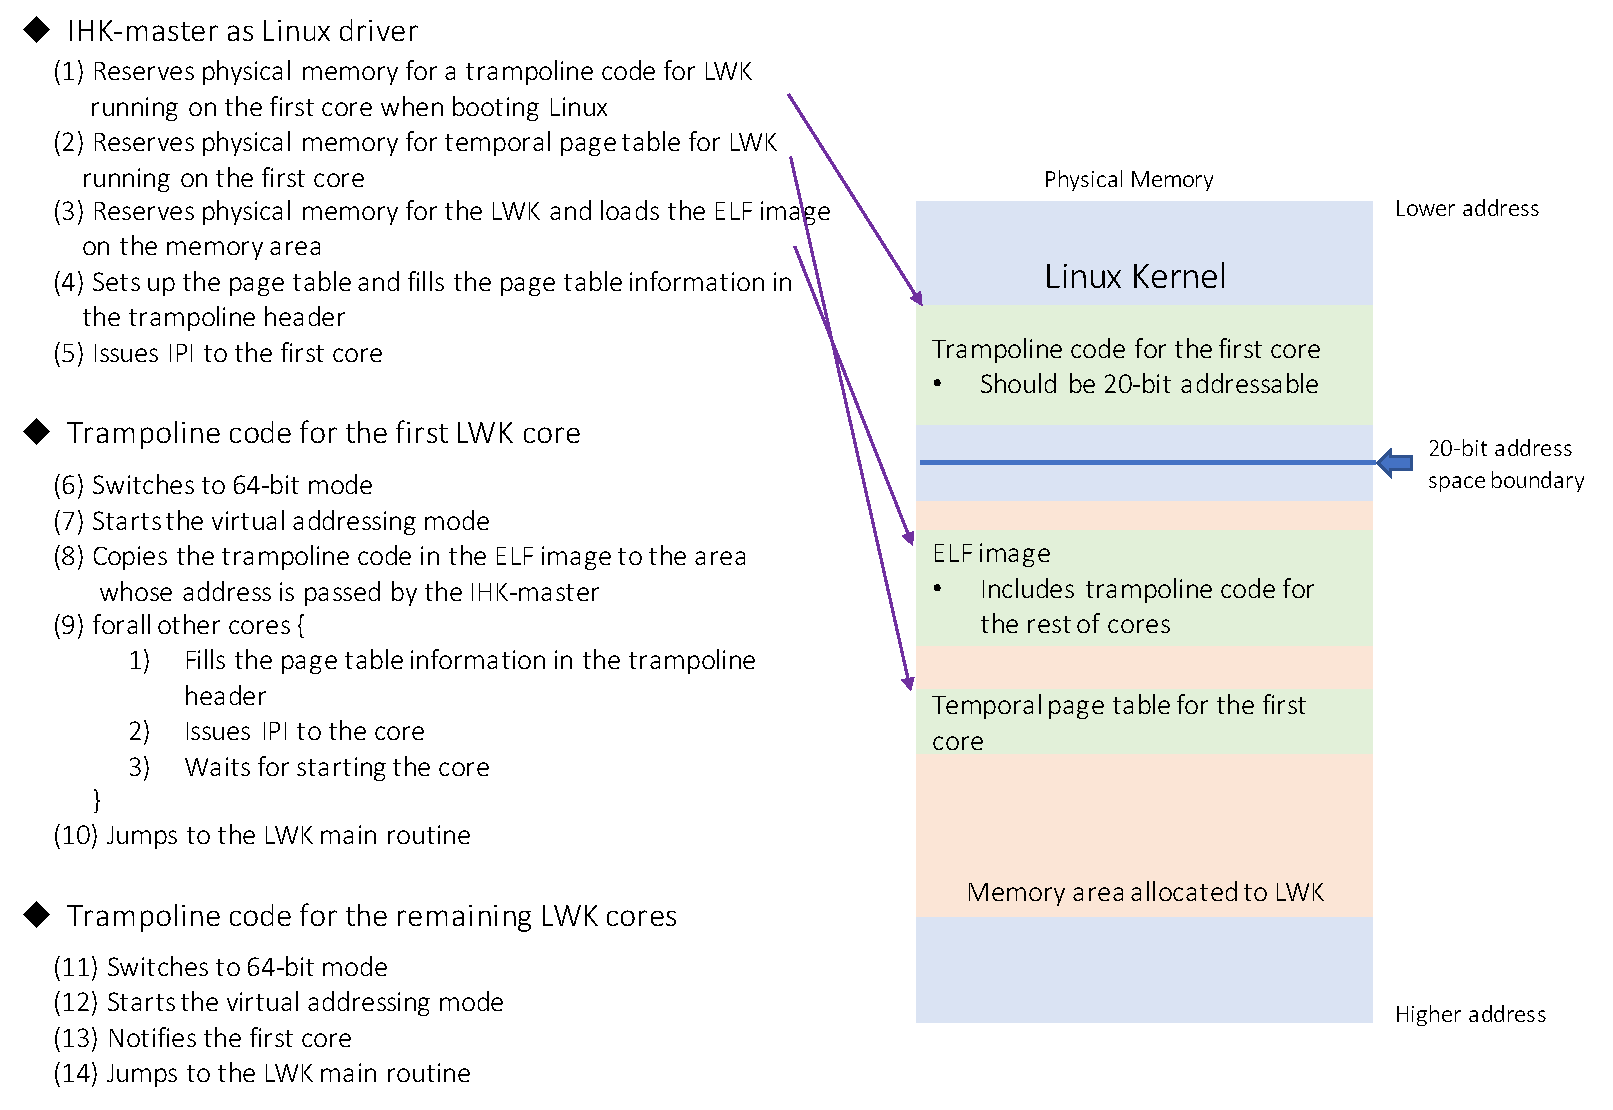
\includegraphics[width=14cm]{figs/booting-sequence.pdf}
\vspace{-0em}\caption{\textbf{Boot sequence of cores for LWK.}}
\label{fig:booting-sequence}
\vspace{-0em}
\end{figure}
Fig. \ref{fig:booting-sequence} explains the steps for Linux to boot an LWK using IHK.
All of these are performed by IHK. Two particular details deserve further discussion.
First, the trampoline code must fit in 20-bit address space because an IPI is used to make the first LWK core jump to the trampoline code and the current x86 restriction for the address field in the IPI demands 20-bit address representation.
%
Second, the location of the temporal page table must fit in 32-bit address space because the control register (CR3) has 32-bit width when a CPU core is in 32-bit mode in the early phase of the trampoline execution.

When the IHK-slave passes the control to the LWK main routine, it is given the physical address of the kernel arguments as the first argument and the physical address of the kernel text as the second argument.
% TODO: Check the source and find where sp points to.
IHK allocates a dedicated page as stack area and the stack pointer is set to that page.
%
\begin{figure}[h]
\centering
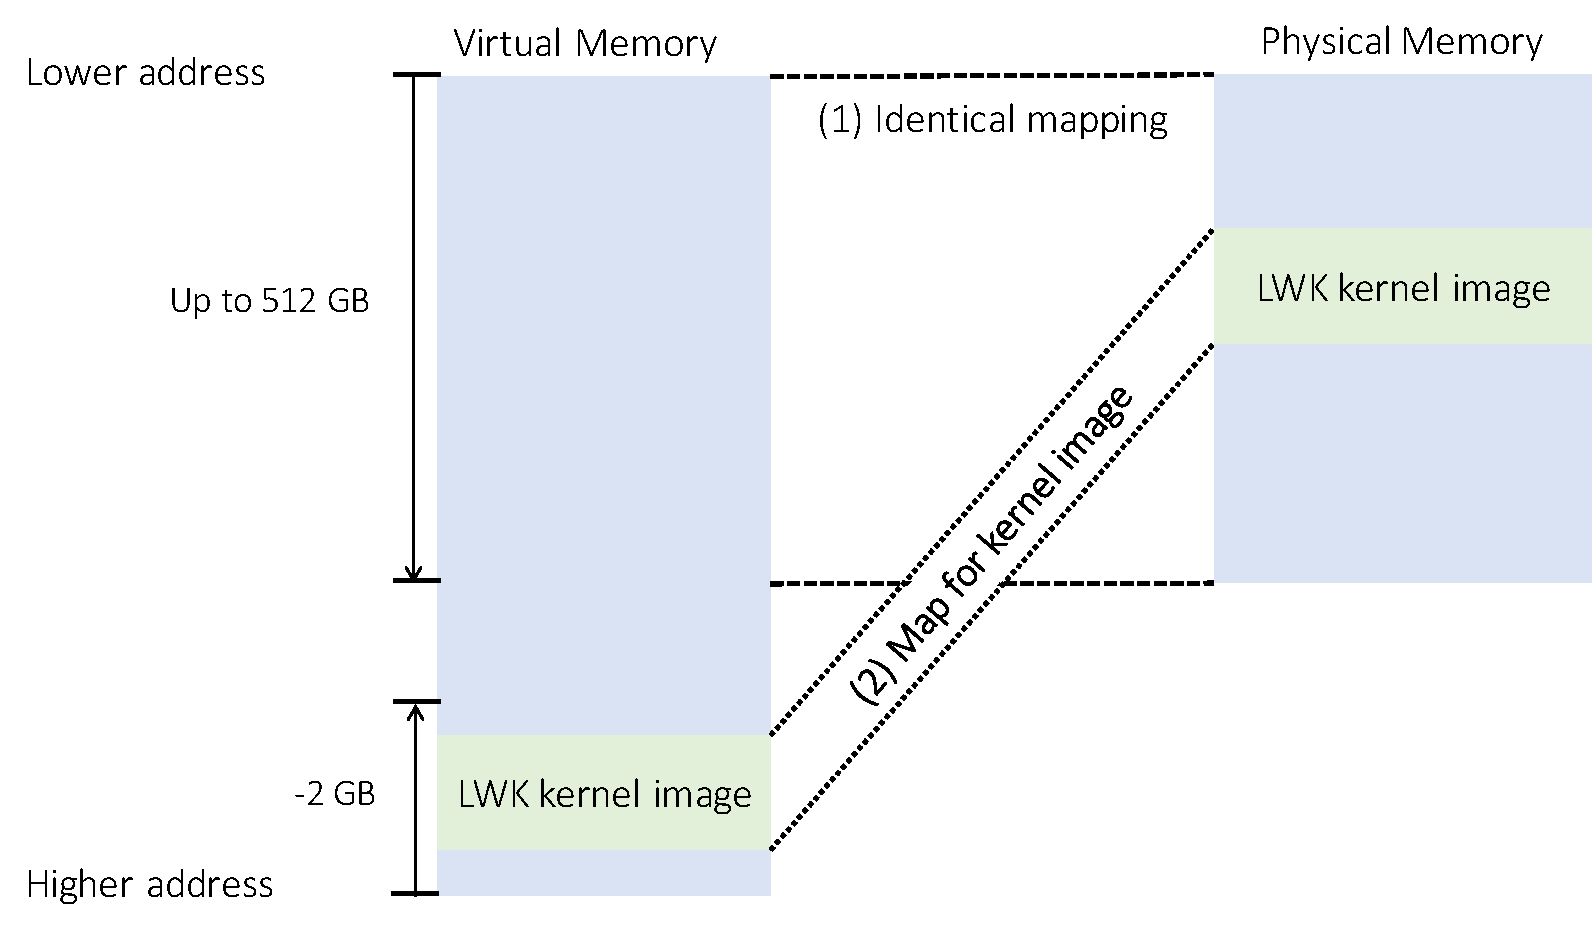
\includegraphics[width=10cm]{figs/memory_map.pdf}
\vspace{-0em}\caption{\textbf{Memory map when the LWK core enters LWK main routine.}}
\label{fig:memory_map}
\vspace{-0em}
\end{figure}
%
Fig. \ref{fig:memory_map} shows the memory map set at the time of entering the LWK main routine.
The virtual address range of \texttt{[ffff ffff 8000 0000, ffff ffff ffff ffff]} points the LWK kernel image in physical address space
and the virtual address range of \texttt{[0000 0000 0000 0000, 0000 ff80 0000 0000]} defines an identical mapping to the same physical address range.
LWK developers are recommended to create their own memory mapping based on this mapping.

%The LWK implementation must retrieve the resource partition information and the kernel argument from IHK, pass kernel-message buffer to Linux and boot other LWK cores using the following IHK functions.
%These functions assume that the virtual address range of \texttt{[ffff ffff 8000 0000, ffff ffff ffff ffff]} points to the LWK kernel image.
% TSS has one dummy entry at this point
% Segment ...
% GDT ...
% IDT ...
% LDT ...
% stack pointer is set to ....


%printglossaries

\bibliographystyle{abbrv}
\bibliography{ihk}

\end{document}
